%!TEX root = ../thesis.tex
%*******************************************************************************
%*********************************** First Chapter *****************************
%*******************************************************************************

\chapter{Introduction}  %Title of the First Chapter

% \ifpdf
%     \graphicspath{{Introduction/Figs/Raster/}{Introduction/Figs/PDF/}{Introduction/Figs/}}
% \else
%     \graphicspath{{Introduction/Figs/Vector/}{Introduction/Figs/}}
% \fi


% \nomenclature[z-cif]{$CIF$}{Cauchy's Integral Formula}                                % first letter Z is for Acronyms 
% \nomenclature[a-F]{$F$}{complex function}                                                   % first letter A is for Roman symbols
% \nomenclature[g-p]{$\pi$}{ $\simeq 3.14\ldots$}                                             % first letter G is for Greek Symbols
% \nomenclature[g-i]{$\iota$}{unit imaginary number $\sqrt{-1}$}                      % first letter G is for Greek Symbols
% \nomenclature[g-g]{$\gamma$}{a simply closed curve on a complex plane}  % first letter G is for Greek Symbols
% \nomenclature[x-i]{$\oint_\gamma$}{integration around a curve $\gamma$} % first letter X is for Other Symbols
% \nomenclature[r-j]{$j$}{superscript index}                                                       % first letter R is for superscripts
% \nomenclature[s-0]{$0$}{subscript index}                                                        % first letter S is for subscripts


%********************************** %First Section  **************************************
\section{The physics of QGP} %Section - 1.1 
\subsection{The strong interaction}
Since the discovery of atomic nuclei and their apparently smallest constituents, at least two topics have been deeply discussed by physicists for decades: are such particles fundamental (and if not how are they formed) and how do they interact?
The first big jump ahead towards the answer was performed in 1961 independently by Gell-Mann and Ne'eman with the eight-fold theory, later developed further as the baryons octet and hyperions decuplet, represented in figure\ref{fig:gelmann}.
The organization of the particles was related to a symmetry group called $SU(3)$ which provides a triplet fundamental representation not observed in nature.
This hint, combined with the speculation that 8 or 10 particles were not likely all fundamental, lead to the introduction of more fundamental particles.

\begin{figure}[!ht]
\begin{center}
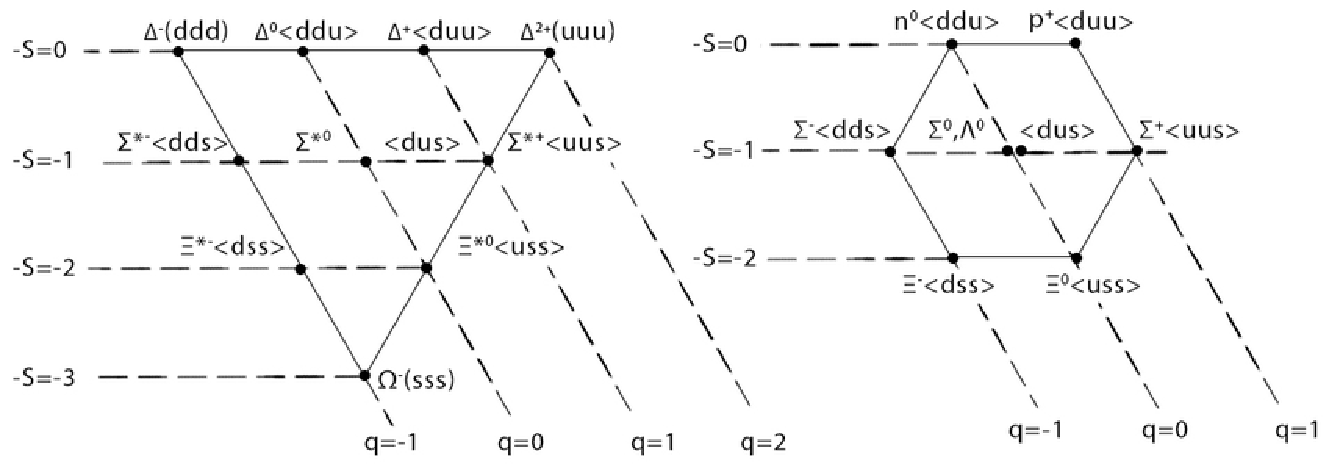
\includegraphics[width=0.8\linewidth]{Chapters/Introduction/Figs/eightfold_way.pdf}
\caption{Representation of the baryon decuplet (left) and octet (right) following the eightfold way approach for three kinds of quarks: up, down and strange. The horizontal levels represent the net strangeness number, while the diagonals (top left to bottom right) link baryons with the same electric charge. From \cite{Akash:2015}}
\label{fig:gelmann}
\end{center}
\end{figure}

They were later called quarks by Gell-Mann.
At a given point Gell-Mann and Zweig argued that, assuming the quarks spin to be $1/2$, mesons could be explained as bound states of a quark and an antiquark, while baryons were a bound state of three quarks.
This choice lead to the peculiar electric charge of $\pm1/3$ and $\pm2/3$.
A last issue regarded the spin statistics theorem violation, solved by the introduction of an additional quantum number: the colour.
This was the birth of the quark model.
By assuming the hadronic matter is not fundamentally made of protons and neutrons they were able to organize in an elegant way the zoo of particles discovered during the $20^{th}$ century.

During the same years, Richard Feynman started thinking about a model useful for analyzing the hadrons produced in high energy physics experiments and capable of interpreting the radiation showers originating in ultra-relativistic collisions.
By introducing the partons and the parton distribution functions, Feynman was able to interpret the deep inelastic scattering on hadrons as the collision between the projectile and an inner constituent of the target, called parton (see Fig.\ref{fig:DIS}).

\begin{figure}[!ht]
\begin{center}
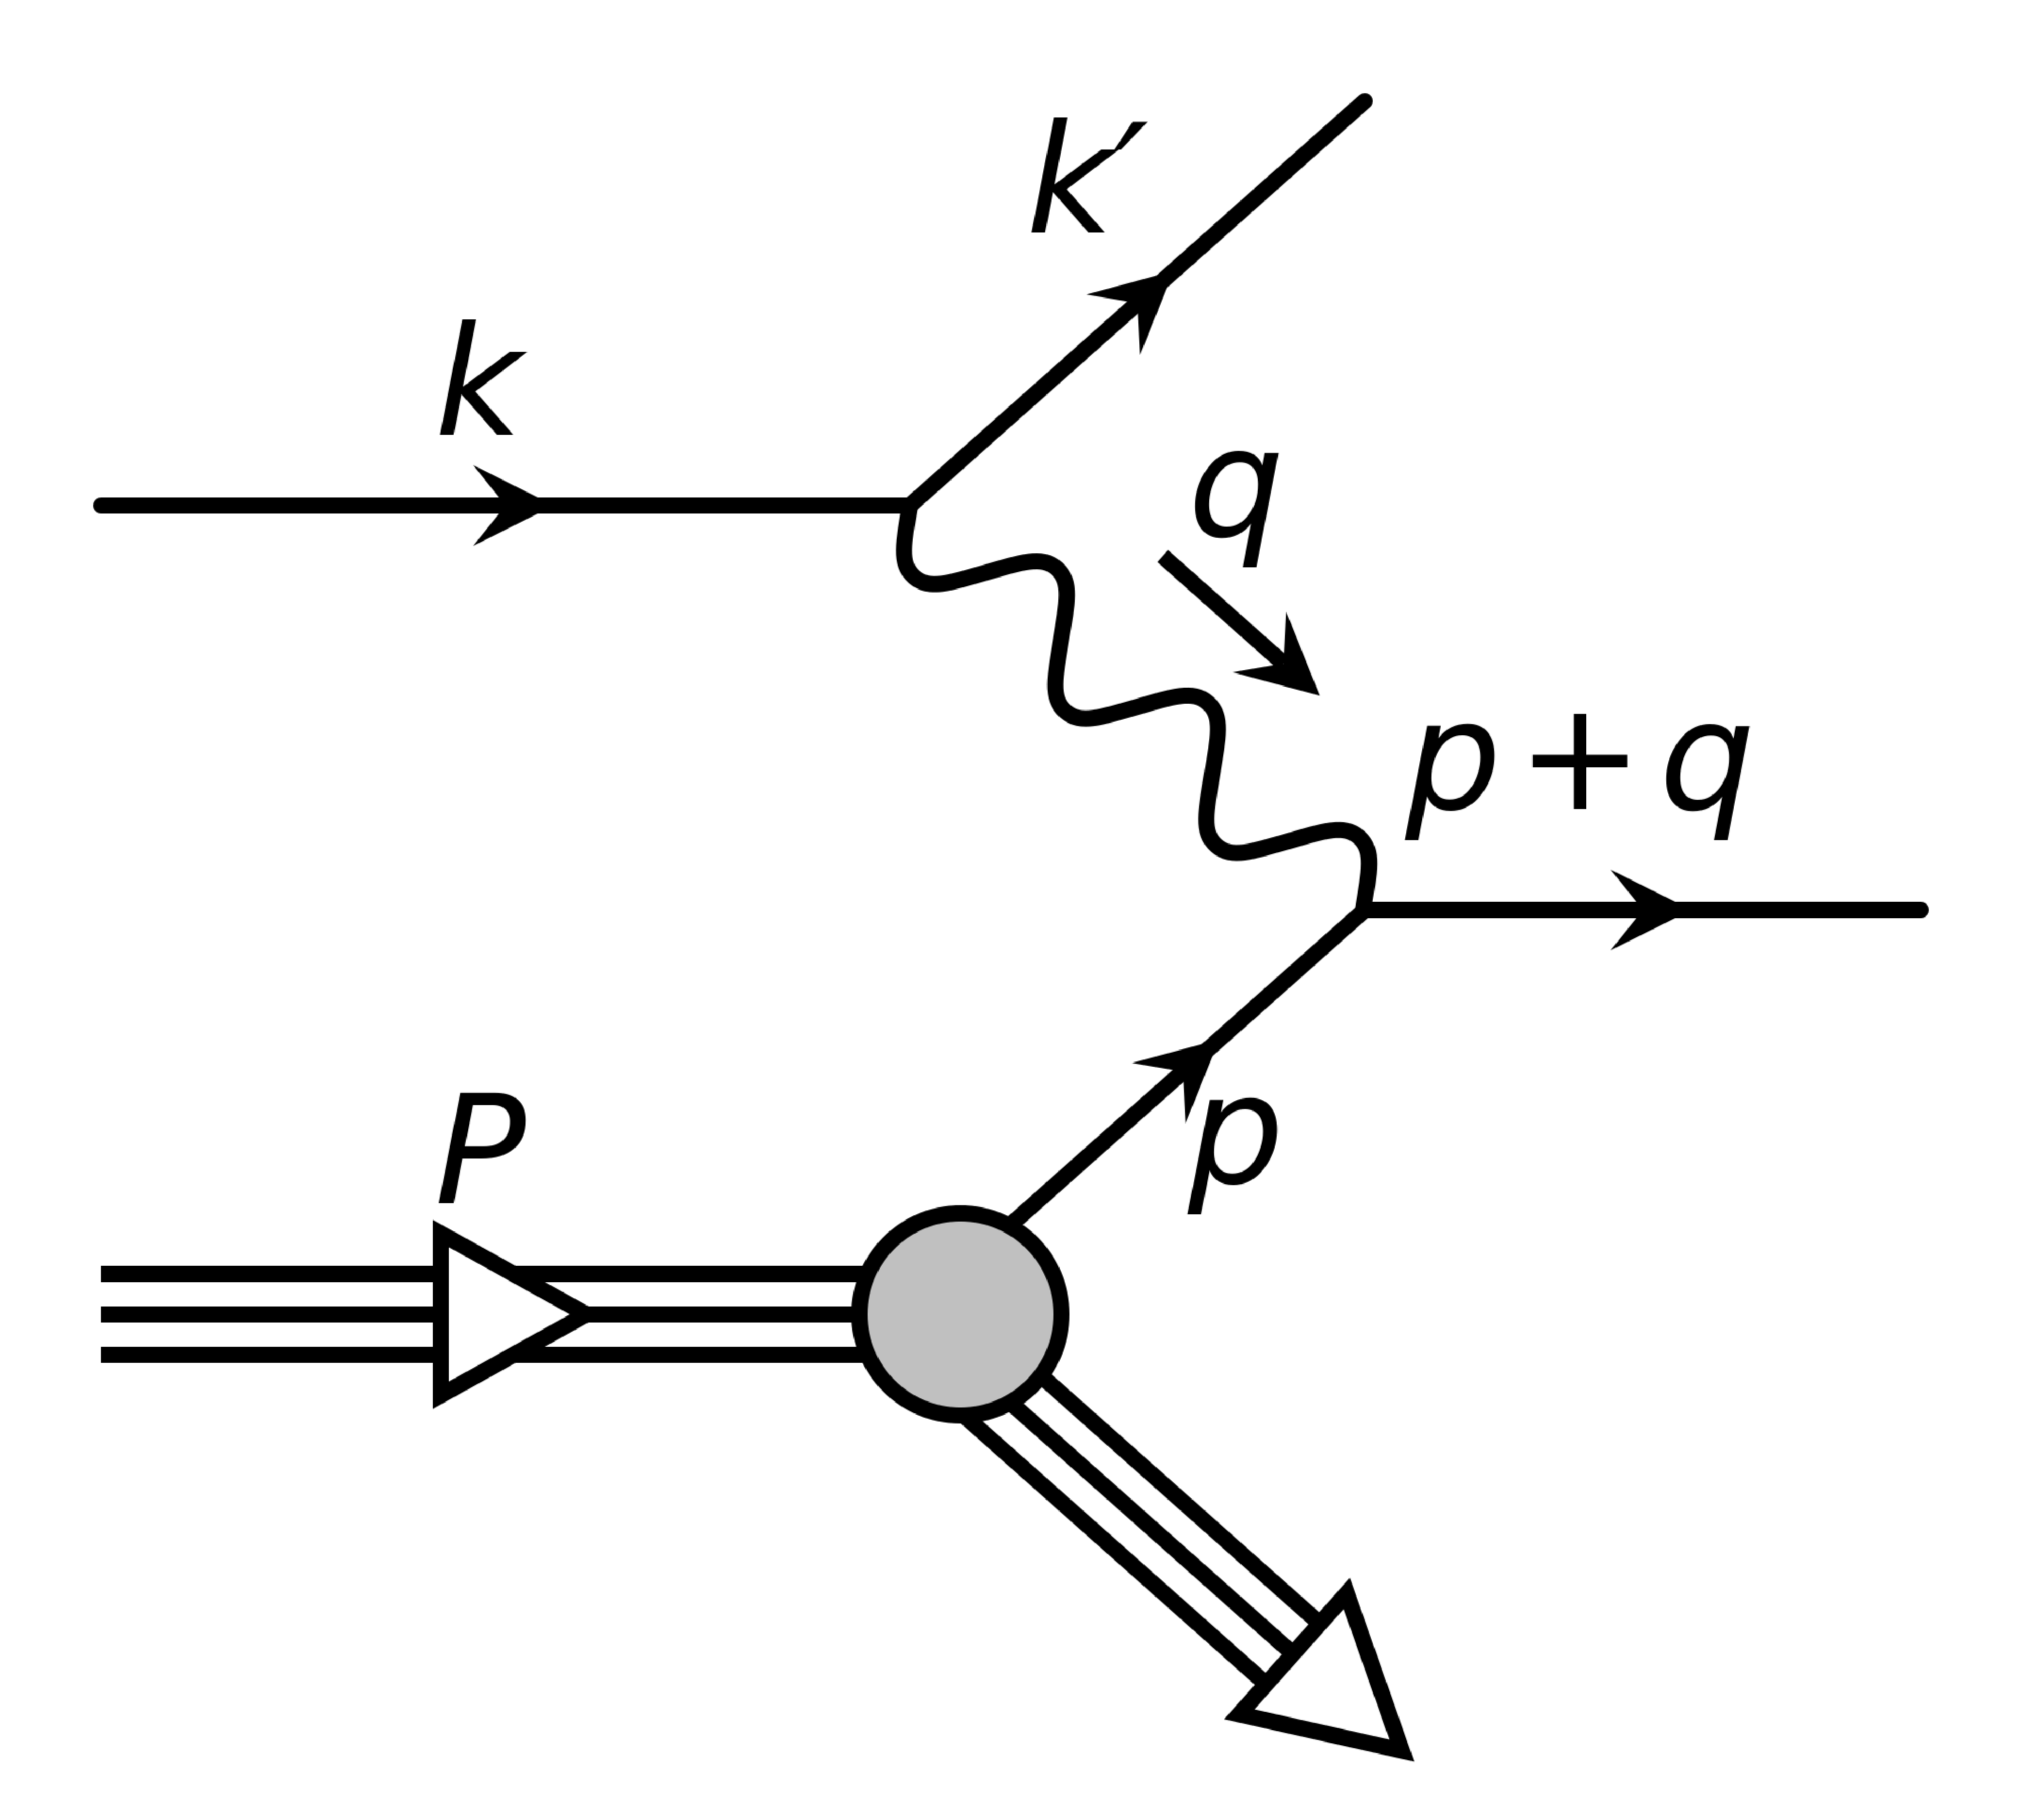
\includegraphics[width=0.5\linewidth]{Chapters/Introduction/Figs/DIS.pdf}
\caption{Cartoon of a deep inelastic scattering process between a projectile of momentum $k$ and $k'$and a parton of initial momentum $p$ belonging to a nucleon of initial momentum $P$. The interaction is mediated through the exchange of a boson of momentum $q$. 
\href{https://commons.wikimedia.org/wiki/File:Deep_inelastic_lepton-hadron_scattering.svg}{[source]}
}
\label{fig:DIS}
\end{center}
\end{figure}

Experiments of deep inelastic scattering performed at the Stanford Linear Accelerator Center (SLAC) between 1967 and 1973 pointed out a scaling behaviour, explained by Bjorken and Feynman as a signature of the point like constituents of the proton.
Bjorken demonstrated that the functions $F_2$ which describes the structure of the nucleon neither depend on the transferred momentum ($Q^2$) nor on the energy transferred in the scattering ($\nu$), but on their ratio\footnote{The observed scaling was a peculiarity of the explored $x$ range ($0.2<x<0.3$), since at higher and lower $x$ ranges the scaling is violated by a dependence of $F_2$ from the transferred momentum $Q^2$.}:

\begin{equation}
    x = \frac{Q^2}{2\cdot M \cdot \nu}
\end{equation}

where $M$ is the mass of the target.
The $x$ variable has no dimension and stands for the ratio between the fraction of the 4-momentum that is transported by the point-like constituent and the total 4-momentum of the target.

\begin{figure}[!t]
\begin{center}
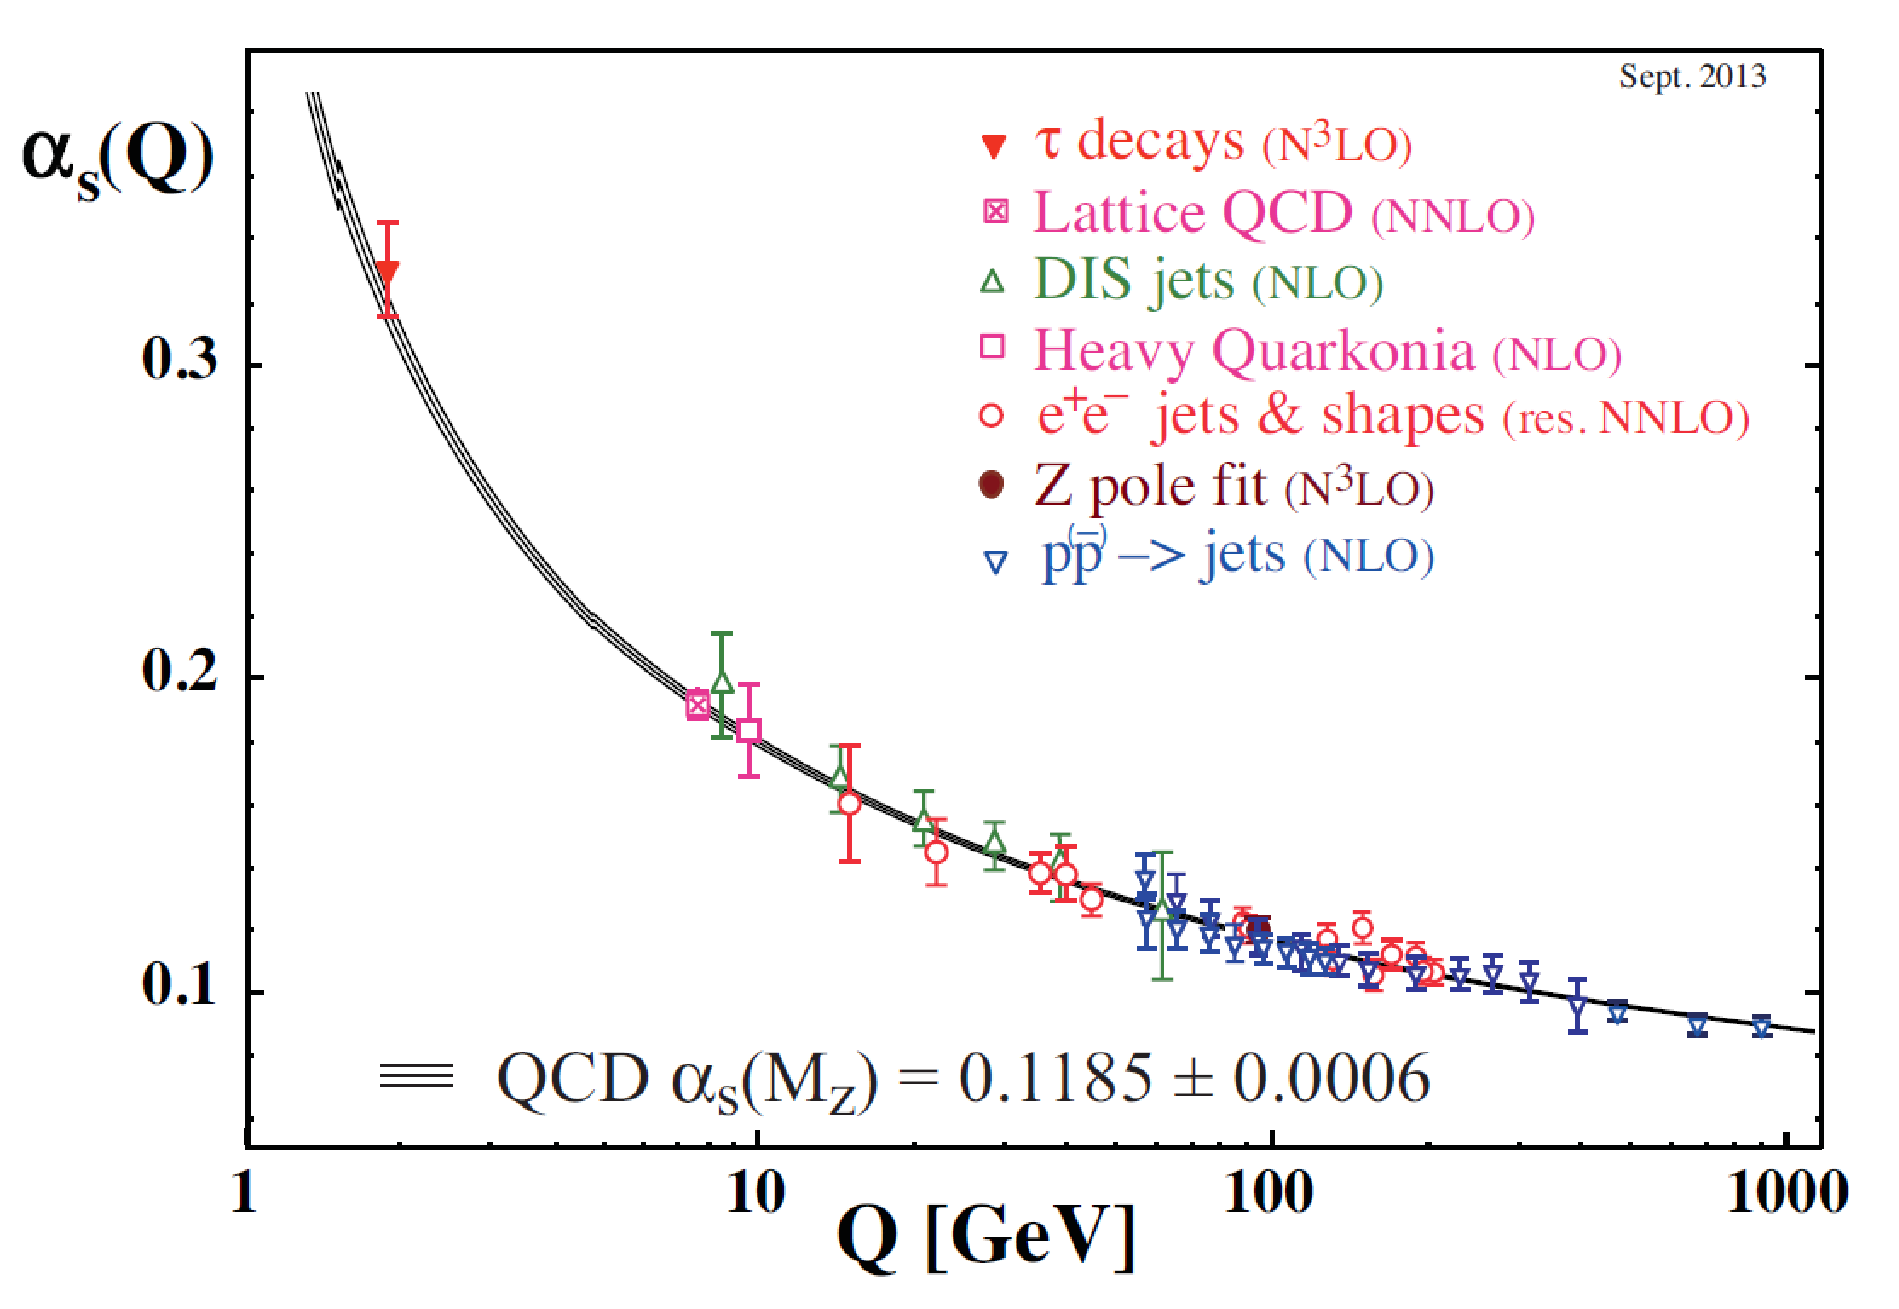
\includegraphics[width=0.85\linewidth]{Chapters/Introduction/Figs/QCD-running-coupling.pdf}
\caption{Plot of the running coupling constant of the strong interaction $\alpha_S$. The band has been computed using the standard model and several experimental points, obtained measuring the coupling from different processes, are shown.}
\href{https://www2.physics.ox.ac.uk/sites/default/files/2014-03-31/qcdgrad_rojo_oxford_tt14_3_rge_pdf_19828.pdf}{[source]}
\label{fig:running}
\end{center}
\end{figure}

After few other proofs the Gell-Mann quarks and the Feynman partons turned out to be the same objects.
The answer to the first question was then well established (how are hadrons made?) when the physics community started tackling the second one regarding how do they interact.
The peculiarity of the new set of particles was the introduction of colour quantum number.
In 1973, in analogy with the Quantum Electro Dynamics (QED), the Quantum Chromo Dynamics (QCD) was proposed as the quantum field theory of the hadronic interaction.
The theory was supposed to be based on the existence of three colour charges and the non-Abelian simmetry group SU(3).
Eight massless bosons, generators of the Lie symmetry group of the strong interaction, represented the mediators of such interaction and were later called gluons.

The gluons are different with respect to the photons, since, as an effect of the non Abelian-ness of the theory, they carry a colour charge, making them self-interacting.
The coupling constant of the strong interaction is defined as running, since it depends on the value of the transferred momentum $Q^2$ as shown in Fig.\ref{fig:running}.
In particular the lower the $Q^2$ values the higher the coupling constant.
As a result, the strength of the interaction increases with distance.
This property leads to the confinement of quarks and gluons inside hadrons.
As a result the hadrons can only be found or produced in a colour singlet state and isolated quarks cannot be observed.

\begin{figure}[!t]
\begin{center}
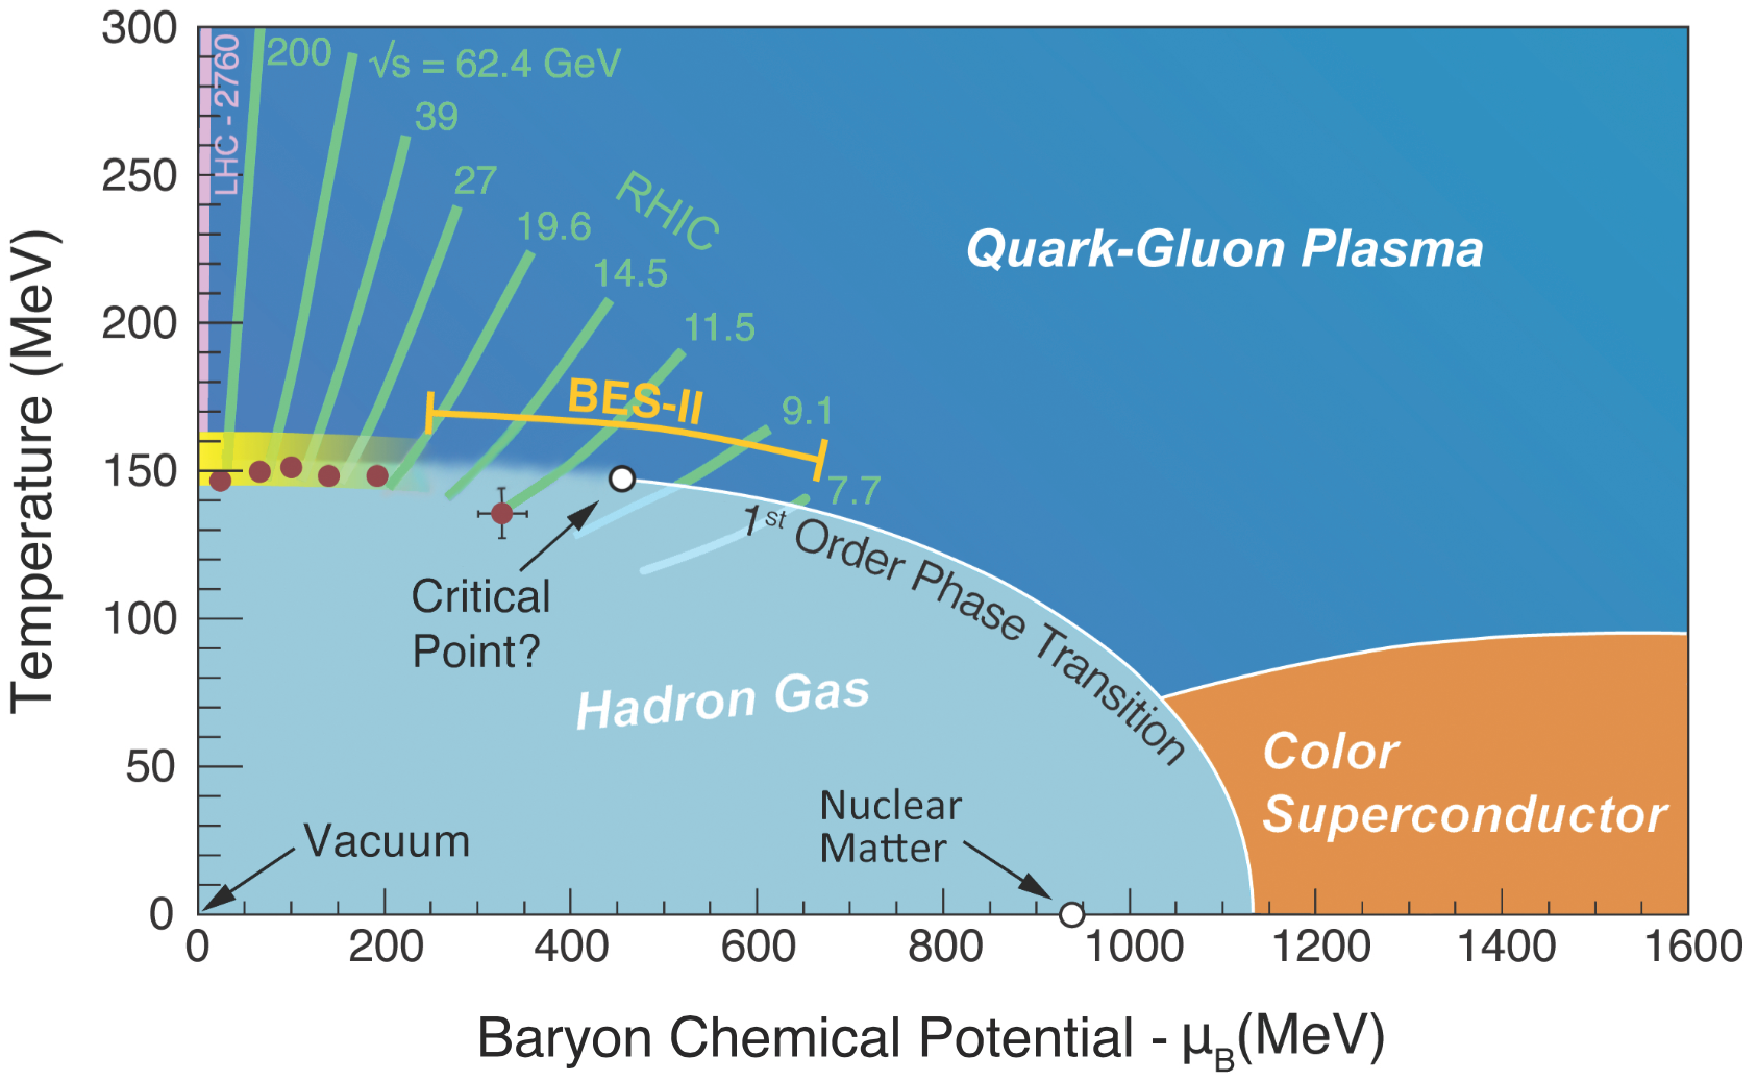
\includegraphics[width=0.85\linewidth]{Chapters/Introduction/Figs/QGPPhases.pdf}
\caption{Cartoon showing the main hadronic matter phases in a $(T,\mu_B)$ diagram.}
\href{https://deixismagazine.org/2016/06/early-universe-soup/dol_plasma/}{[source]}
\label{fig:QGPPhases}
\end{center}
\end{figure}

\subsection{Quark Gluon Plasma}
In 1975 N. Cabibbo and A. Parisi \cite{Cabibbo:1975ig} suggested a state of nuclear matter in which quarks and gluons are not confined anymore into hadrons to explain the exponentially increasing spectrum proposed by Hagedorn \cite{Hagedorn:1965st}.
This new state of matter was later called Quark Gluon Plasma (QGP).
From theoretical studies the main parameters determining the QGP evolution are the temperature (T) and the baryon-chemical potential ($\mu_B$), defined in a thermodynamical fashion as the derivative of entropy with respect to the net baryon number.
Three main regions are spotted in the $(T,\mu_B)$ phase diagram represented in Fig.\ref{fig:QGPPhases}:
\begin{itemize}
    \item At low T and low $\mu_B$ the nuclear matter is composed of hadrons behaving as a hadron gas;
    \item At low T and high $\mu_B$, according to the latest theoretical developments, quark matter should enter a phase other than QGP, analogous to the superconducting phase of solid-state physics \cite{Alford:2007xm};
    \item At high T the strongly interacting matter can be described as a system of deconfined partons. Such behaviour is caused by the asymptotic freedom of QCD.
\end{itemize}

According to the Big Bang model the conditions of high temperature and low baryon-chemical potential are supposed to be the ones of the early Universe.
At the beginning of the Universe all the energy and matter were condensed in a tiny spatial region.
Then, during the first microseconds of evolution, the Universe started expanding from a condition of extreme energy density and temperature.
Indeed the extreme conditions needed for the QGP production are similar to the ones happened at the beginning of the Universe evolution and can be reproduced in laboratory by means of ultra-relativistic heavy ion collisions.

While expanding, the energy density and the temperature started dropping.
Two transitions happened at $T\simeq160$ MeV and $T\simeq100$ KeV \cite{Kapoyannis:2017hcz}: the hadron formation started at the first threshold, while small nuclei could survive after the second value \cite{Dumitru:2000sc}.
The nuclear composition of early Universe was fixed at that point: such phenomenon is called primordial nucleo-synthesis.
Only few minutes later, when the Universe temperature dropped below $1$ MeV, the radiation decoupled from matter and the whole Universe started becoming transparent.
The Cosmic Microwave Background (CMB) is the residual of the first radiation.

Studying the QGP evolution and its characteristics might lead to a better understanding not only of the strong nuclear interaction and the origin of hadron masses, but also of the process of Universe formation.

One of the most common phenomenological models which can be cited to describe the transition to QGP is the MIT bag model \cite{PhysRevD.9.3471,PhysRevD.10.2599}.
The two main hypotheses of this model are:
\begin{itemize}
    \item the quarks are massless particles put inside a bag of finite dimension;
    \item the confinement originates from the balancing of the internal pressure exerted by quarks into the bag and an external pressure $B$;
\end{itemize}
The total energy of $N$ quarks confined in a spherical volume of radius $R$ is the sum of a kinetic term and a term related to the compensation by the external pressure $B$:
\begin{equation}
    E=\frac{2.04\cdot N}{R}\cdot \hslash c + \frac{4\pi}{3}\cdot R^3\cdot B
\end{equation}
The bag radius is determined by finding the minimum of energy of the system.
Such condition is obtained imposing the condition $dE/dR=0$.
\begin{equation}
\frac{dE}{dR}=-\frac{2.04\cdot N}{R^2}\cdot \hslash c + 4\pi\cdot R^2\cdot B = 0
\end{equation}
The model allows one to compute confinement thresholds for various systems.
For example, for a baryon, composed by $N=3$ quarks and with $R=0.8$ fm the external pressure becomes:
\begin{equation}
B^{1/4} = \frac{206\ \mathrm{MeV}}{\hslash c}
\end{equation}
Such value is the limit below which the confinement of the quarks inside the baryon happens.
% If the internal pressure grows above such threshold the quarks start behaving as asymptotically free.
With the growth of the internal pressure, the quarks behaviour gradually changes to an asymptotically free one.
The internal pressure can increase in two ways:
\begin{itemize}
\item The increase of temperature causes an increase of kinetic energy of quarks inside the bag. In this situation the formed QGP is called "hot";
\item The increase of pressure is caused by the increase of baryon density achieved via compression. This scenario is possible in extremely dense objects such as neutron stars and is defined as "cold" QGP.
\end{itemize}

The bag model provides an estimation of the minimum temperature and energy density needed to produce the deconfined state.

The pressure required to produce a QGP out of a volume $V$ filled with massless quarks and gluons in which the net baryon number is null (equal number of quarks and anti-quarks) is computed as:
\begin{equation}
P = g_{tot}\cdot\frac{\pi^2}{90}\cdot T^4
\end{equation}
Where $g_{tot}$ is the total number of degrees of freedom for quarks, anti-quarks and gluons.
The pressure exceeds the external one at a temperature of around $145$ MeV, a value similar to the lattice-QCD prediction of $160$ MeV \cite{Kapoyannis:2017hcz}.
In addition, since the energy density is related to the pressure value, it can be computed as well:
\begin{equation}
\epsilon = 3\cdot P = g_{tot}\cdot\frac{\pi^2}{30}\cdot (160\ \mathrm{MeV})^4 \simeq 1\ \mathrm{GeV/fm^3}
\end{equation}
Which is considered to be the threshold value to produce a deconfined medium.

\begin{figure}[!t]
\begin{center}
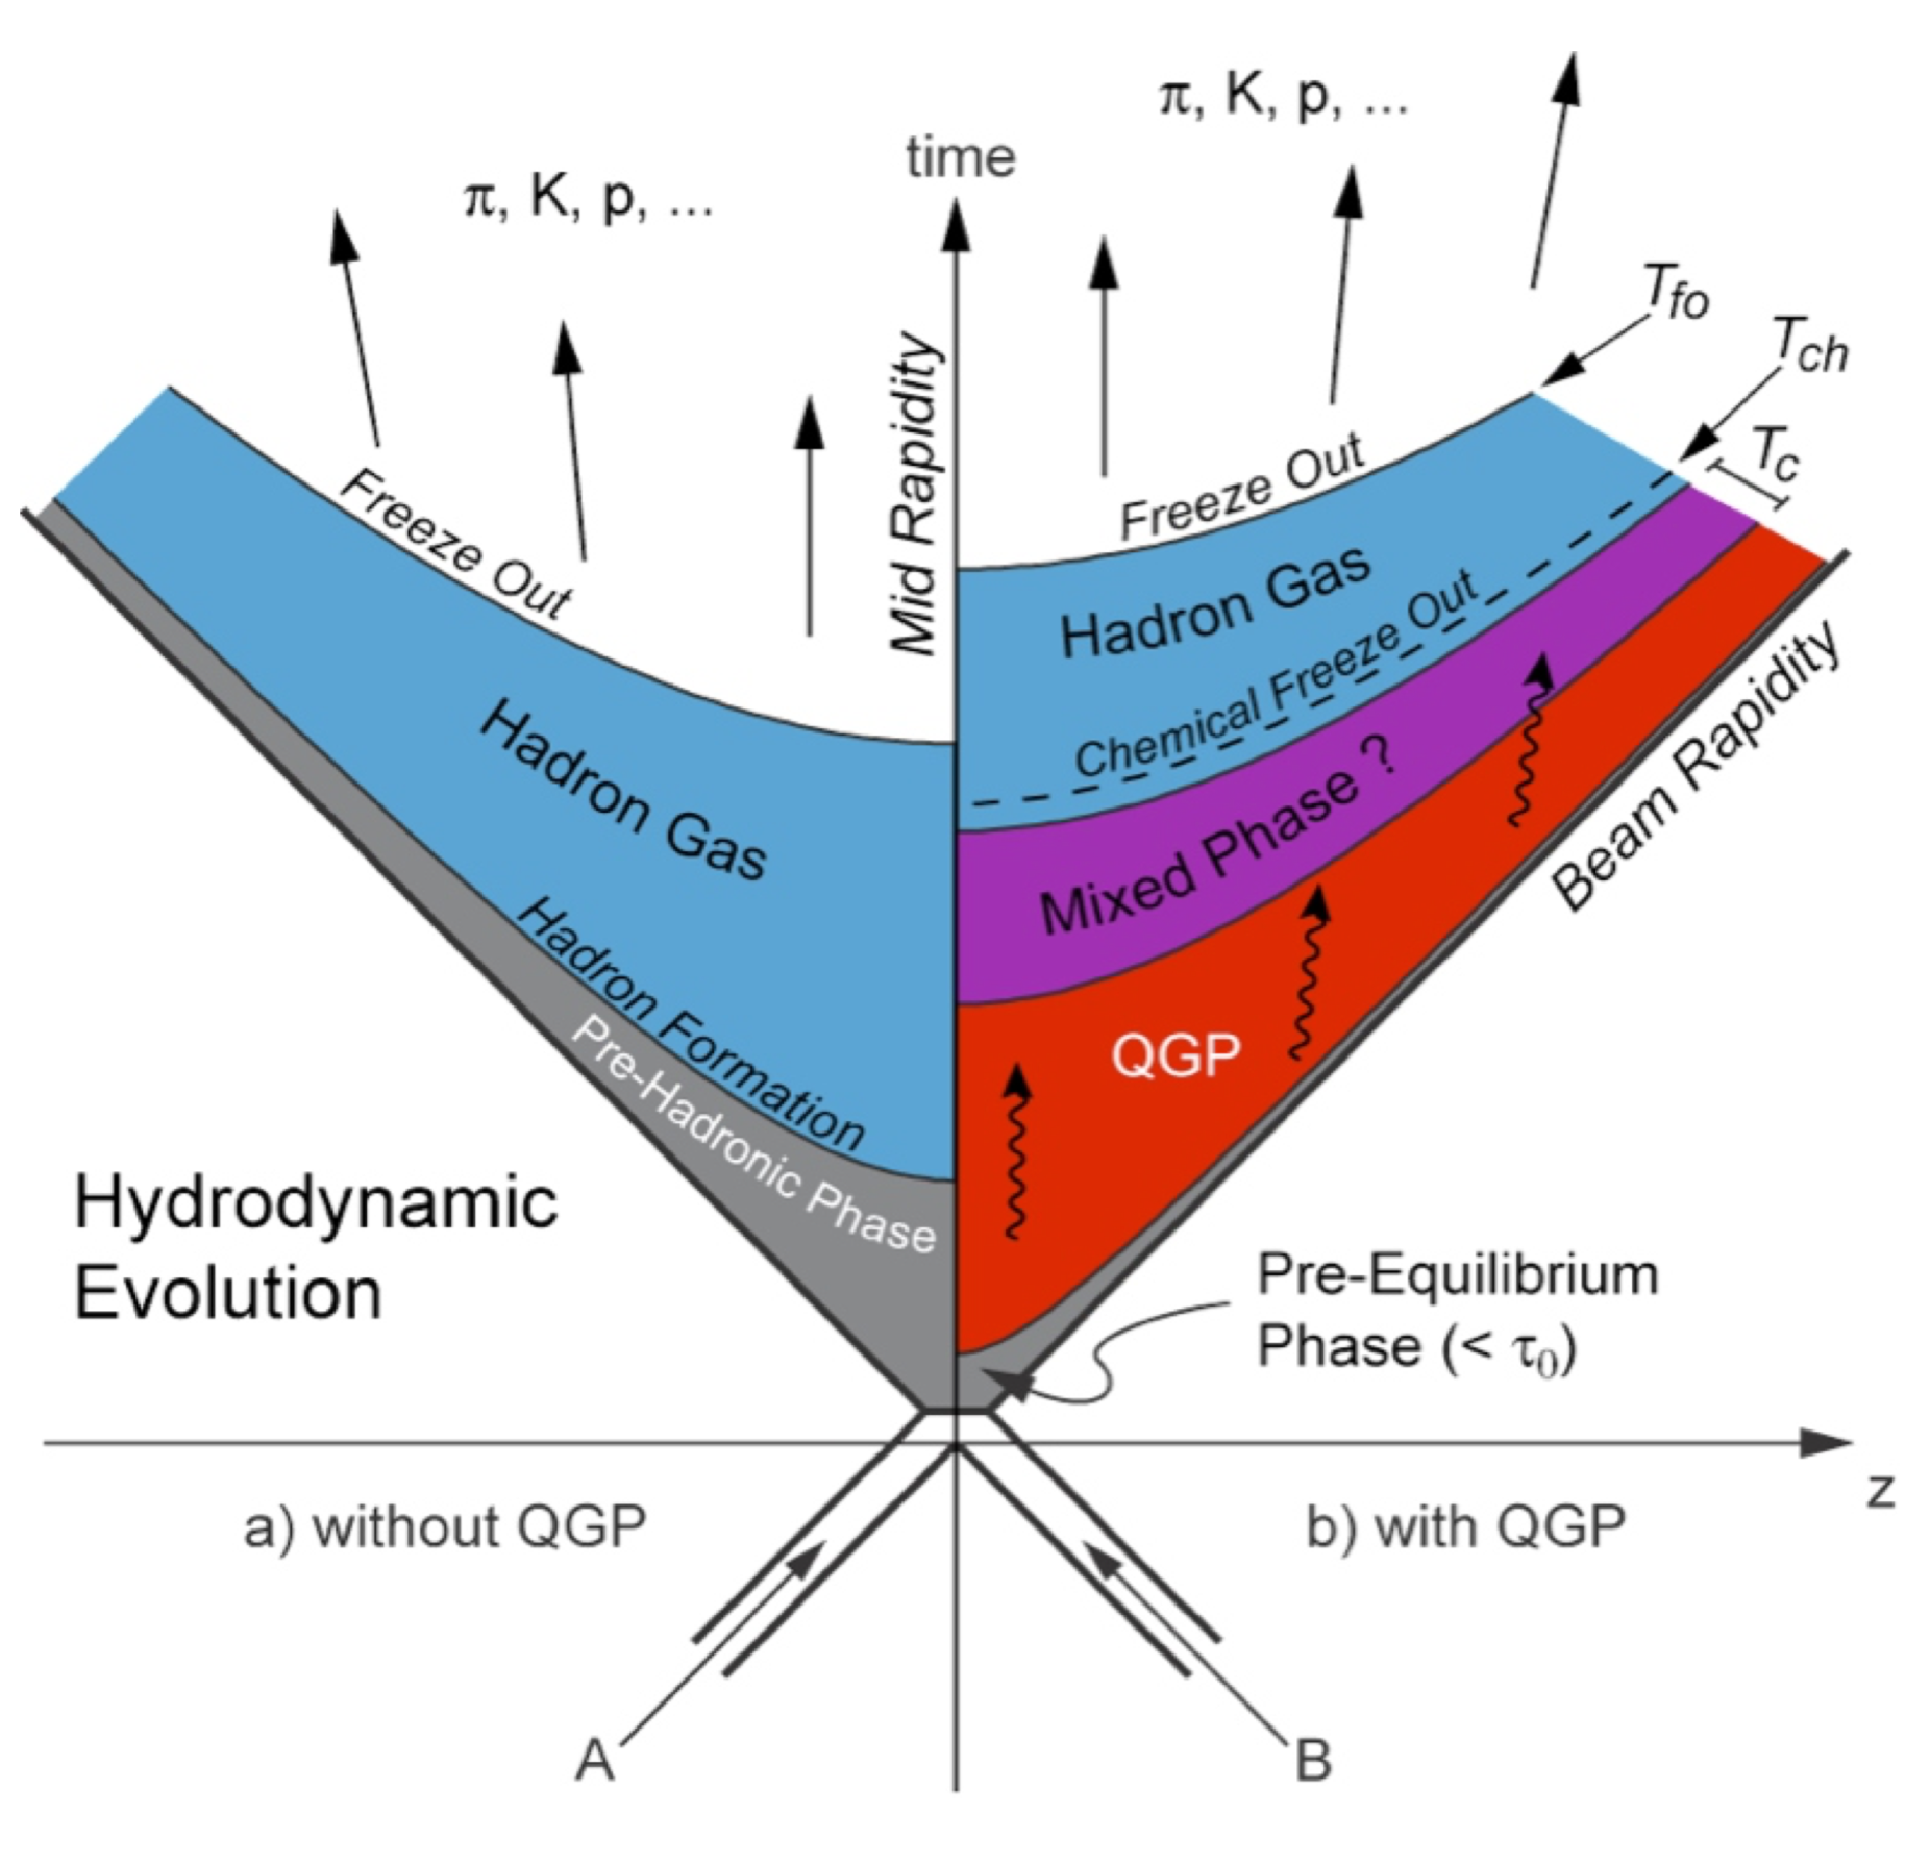
\includegraphics[width=0.85\linewidth]{Chapters/Introduction/Figs/QGP_evo.pdf}
\caption{Space-time evolution of the fireball originated from an heavy ion collision with (left) and without (right) QGP.}
\href{https://www.physi.uni-heidelberg.de/~reygers/lectures/2015/qgp/qgp2015_06_space_time_evo.pdf}{[source]}
\label{fig:evolution}
\end{center}
\end{figure}

The heavy-ion collision experiments tackle the QGP production through the approach based on reaching an extreme temperature, thanks to the high energy available in the center of mass of the collision.
% The computed threshold can be crossed in ultra-relativistic heavy ion collisions.
The collision process is characterized by a complex space and time evolution, but can be divided in some macro-conditions which can help understanding the whole process (see Fig. \ref{fig:evolution}):
\begin{itemize}
    \item at $t=0$ the collisions process starts;
    \item Right after the collision the system crosses a pre-equilibrium phase. During this phase the medium is not yet thermalized and is governed by hard and semi-hard QCD processes;
    \item The central "fireball" starts expanding following pressure gradients. The partons act as deconfined during this phase. The conservation of energy causes the temperature to drop depending on the fireball expansion;
    \item The chemical freeze-out happens when the average temperature drops below a threshold which at LHC amounts to $\simeq160$ MeV \cite{Kapoyannis:2017hcz}. The energy of the interactions does not allow to modify the abundances of hadrons;
    \item The thermal freeze-out corresponds to the moment in which the elastic interactions between hadrons stop. At this point the kinematic spectra of the produced hadrons is fixed. The threshold temperature for this situation was deduced to be around $120$ MeV \cite{Mukherjee:2012fb}.
\end{itemize}

The QGP phase lasts for about $10$ fm/c and a direct observation is impossible.
However, after the thermal freeze-out the hadrons fly freely and they can be detected by the experiment.
Since the emerging hadrons had been influenced by the interaction with the QGP, or even produced inside it, they carry valuable information on its properties.

\subsection{Soft and hard probes}
The particles produced in a nuclear collision might be distinguished in soft and hard probes.
Soft probes are produced during the evolution of the system formed in the collision and are related to the collective behaviour of the medium.
The processes involving a soft probe production are characterized by low transferred momentum and for this reason most part of the produced particles are soft probes.
Some observables related to soft probes are:
\begin{itemize}
    \item Particle multiplicity: the multiplicity of particles produced is important for the determi- nation of the energy density of the collision and the study of their transverse momentum spectra allows to obtain information on the chemical and thermal freeze-out;
    \item Collective flow: the spatial anisotropy of the colliding region induces pressure gradients which cause anisotropic particle distributions. This effect can be explained as a collective motion of particles produced in the interaction and its study is closely related to the determination of the equation of state for a deconfined medium;
    \item the study of real and virtual photons (electromagnetic probes) is important for the determination of the medium temperature.
\end{itemize}
By contrast to soft probes, hard probes are particles produced in high transferred momentum processes and they are characterized by much lower production cross section.
Hard probes are produced early during the collision and experience the full evolution of the system, in particular the early stage of the deconfined medium.
Some observables related to hard probes are:
\begin{itemize}
    \item Jet quenching: jets are produced by the fragmentation of high momentum partons. Interacting with a deconfined medium they can lose energy scattering with other free partons or through radiative gluon emission. The result is a quenched particle spectrum;
    \item Open heavy flavour: particles with valence heavy quarks (charm or bottom) content are very important in the study of the QGP.
    Heavy quarks are produced in the initial stages of the collisions and experience the full evolution of the fireball.
    They lose energy in the interaction with the medium, and this results in a modification of the differential spectra.
    Moreover, the study of heavy flavours at low pt provides information on the thermalisation process of the medium;
    \item Quarkonia production modification: the term quarkonium indicates a bound state of two heavy quarks and it is named charmonium when formed by charm quarks, bottomomium when formed by bottom quarks. These mesons are strongly affected by the formation of a partonic medium and this effect can result in a suppression due to a mechanism of color screening.
\end{itemize}

The measurement of bottomonium production is a main subject of this thesis.
Similarly to other probes of the system, it can be studied as a function of the centrality of the collision, which allows to access additional information regarding the dependence of the probe production from the energy density.

\subsection{Centrality estimation: Glauber model}
\label{intro_glauber}

\begin{figure}[!ht]
\begin{center}
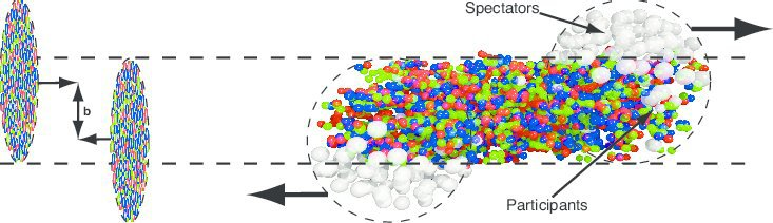
\includegraphics[width=0.99\linewidth]{Chapters/Introduction/Figs/collision.pdf}
\caption{Schematic of the stages on a heavy ion collision surrounding the collision moment. At first (left side) the nuclei are relativistically contracted. After the collision (right side) the spectators proceed unperturbed while the participants generate a colour tube filled of free partons.}
\label{fig:collision}
\end{center}
\end{figure}

In the centre of mass system of the collision, the nuclei are Lorentz-contracted as shown in figure \ref{fig:collision}.
Nuclei are composed by nucleons. The number of nucleons interacting during the collision depends on the impact parameter, which is defined as the spatial separation between the centroids of the two nuclei and determines the number of nucleons participating to the interaction.
The measurement of the impact parameter is fundamental to know the nature of the initial collision state.
The Glauber model, named after Roy Glauber, is usually used to model and analyze the geometry of a nuclear collision.
The model stands on three basic assumptions:
\begin{itemize}
\item At high energy the nucleons are undeflected thanks to the large momentum, hence their trajectory is asymptotically linear;
\item Nuclear size has to be large compared to the range of nucleon-nucleon interaction;
\item Nucleons motion is independent from the nucleus one, hence the nuclear collision can be described in terms of the nucleon-nucleon cross section.
\end{itemize}

% As one can already argue, the Glauber's approach to the description of nuclear collisions simplifies the problem diving to a more fundamental description, given at the nucleon level.
For doing so two inputs are necessary:
\begin{itemize}
\item Inelastic nucleon-nucleon cross section. 
This value should be measured at the same center-of-mass energy. 
It can be measured in proton-proton collisions;
\item Nucleus density profile. It is necessary to provide a contour shape for the colliding nuclei. 
Historically the nucleus profile has been modeled in the shell model approach as a Woods-Saxon distribution, which models the average nucleon potential in the nucleus. 
The potential shape corresponds to the nucleons distribution.
The modified Woods-Saxon distribution, also called 2-parameter Fermi distribution, is:

\begin{equation}
\label{eq:WoodsSaxon}
\rho(r) = \frac{\rho_0\cdot(1+\omega r^2/R^2)}{1+\exp(\frac{r-R}{a})}
\end{equation}

where:
\begin{itemize}
\item $r$ is the radial position at which one wants to compute the nucleons density;
\item $\rho_0$ is the normalization factor needed to provide the correct density value at $r=0$;
\item $\omega$ is a parameter which can represent a density bump right before the distribution tail;
\item $R$ is the radius at which $\rho/\rho_0=\frac{1+\omega}{2}$, similar to a half-width half maximum if $\omega=0$;
\item $a$ describes the steepness of the distribution's tail.
\end{itemize}
The Woods-Saxon distribution parameters are typically determined via $e^-$-nucleus scattering processes.
The differences between protons and neutrons are assumed to be negligible.
In figure \ref{fig:WoodsSaxon} the distribution for a $Pb$ nucleus is shown.

\end{itemize}

\begin{figure}[!h]
\begin{center}
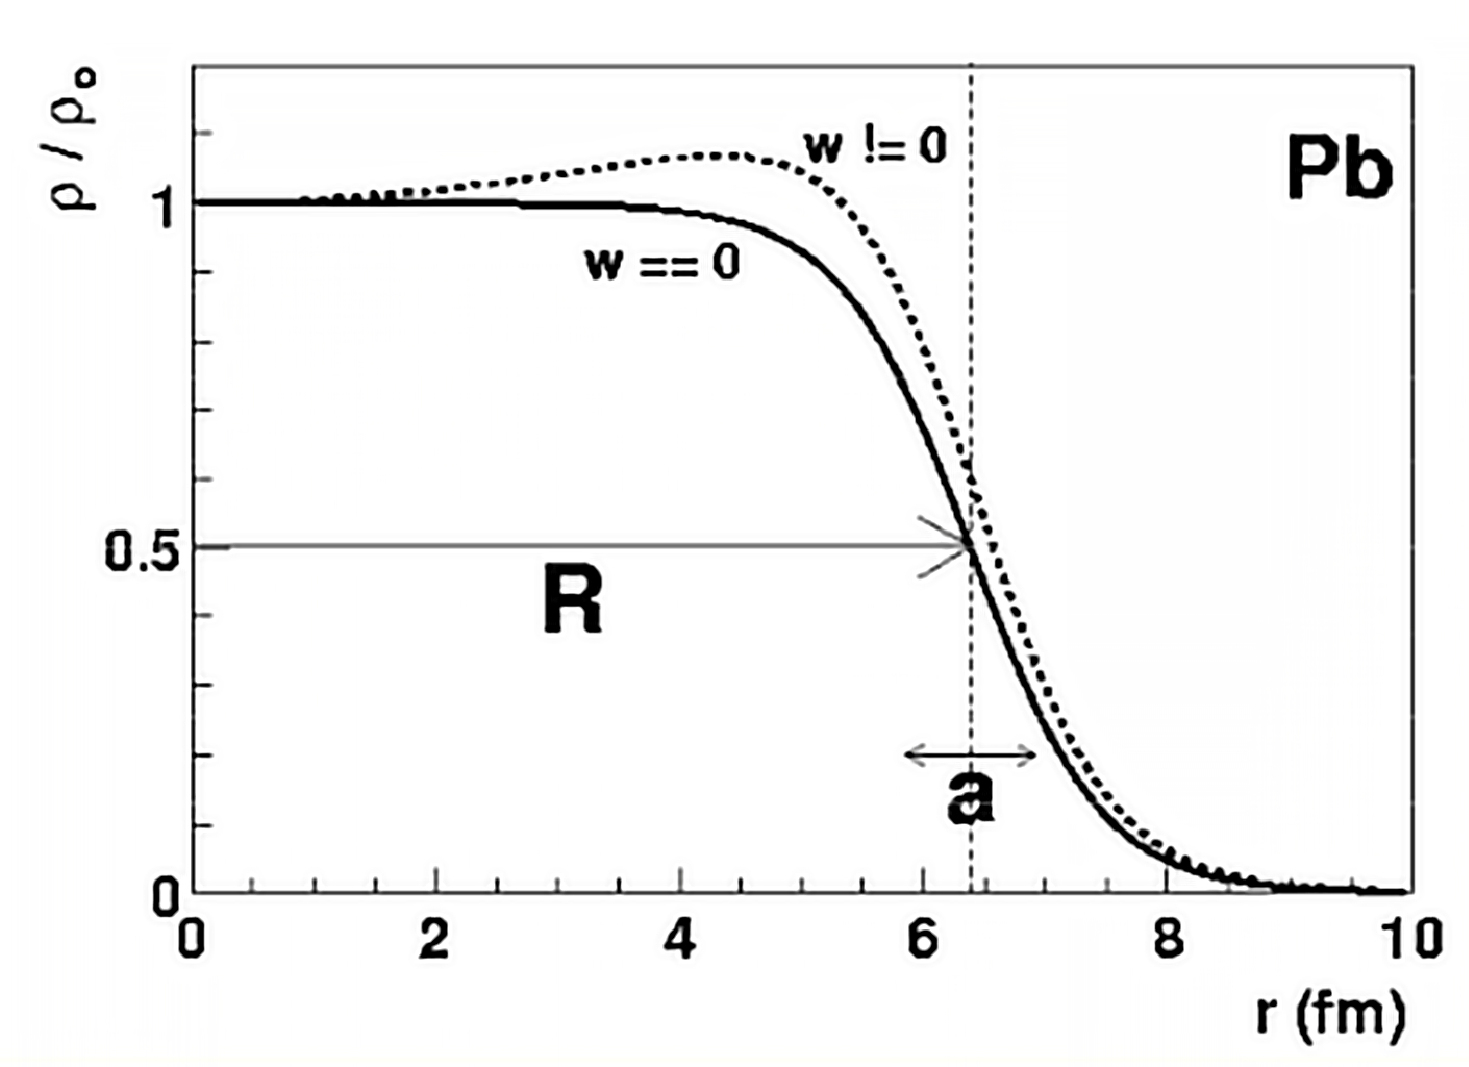
\includegraphics[width=0.7\linewidth]{Chapters/Analysis/Figs/woods-saxon.pdf}
\caption{Woods-Saxon potential for $Pb$ nucleus as the ratio of the $\rho(r)$ over $\rho_0$ as a function of the distance from the nucleus center ($r$).
Displayed parameters are extensively described in paragraph \ref{intro_glauber}}
\label{fig:WoodsSaxon}
\end{center}
\end{figure}

The Glauber model uses an optical and geometric approach to represent the nuclear collision.
Referring to figure \ref{fig:GlauberSide}:
\begin{itemize}
\item $b$ is the distance between the centers of the colliding nuclei, namely the impact parameter;
\item $s$ is the distance of a nucleon flux tube relative to the nucleus center.
\end{itemize}
Note that in this discussion the vectors $\vec{b}$ and $\vec{s}$ will be replaced by their modulus.
This can be done if the colliding particles are not polarized or present a spherical distribution of probability for the nucleon density.
This assumption is legitimate for Pb nuclei.

\begin{figure}[!h]
\begin{center}
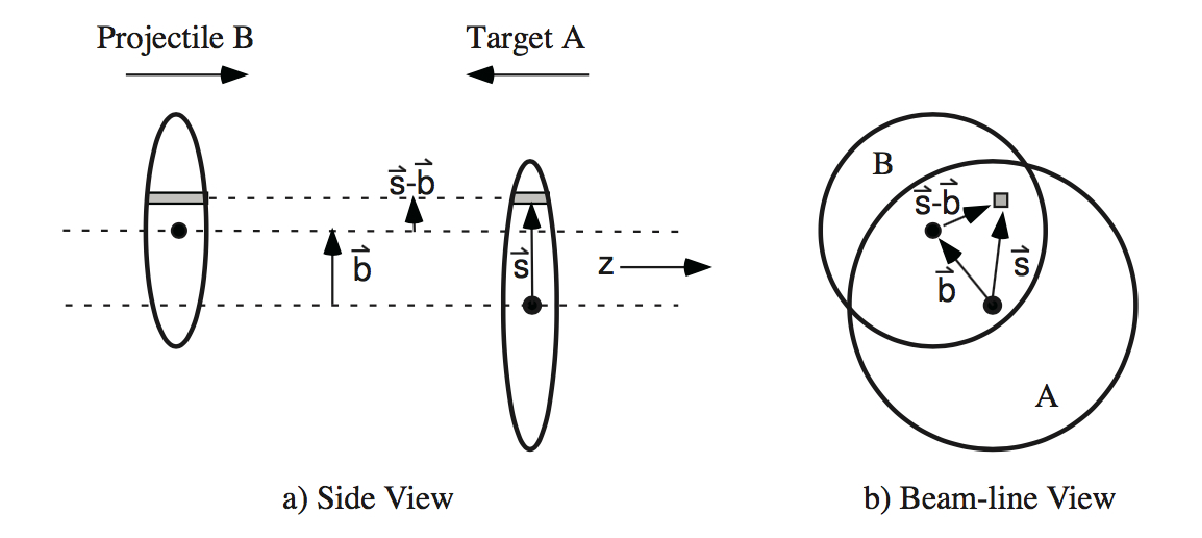
\includegraphics[width=0.85\linewidth]{Chapters/Analysis/Figs/glauber-side.pdf}
\caption{Schematic representation of the Optical Glauber Model geometry, with transverse (a) and longitudinal (b) views. From \cite{Miller:2007ri}.}
\label{fig:GlauberSide}
\end{center}
\end{figure}

The probability of finding a nucleon in a nucleon flux tube positioned at $s$ from target A is defined as:
\begin{equation}
\label{eq:TAs}
\hat{T}_A(s) = \int{\rho}_A(s,z_A)dz_a
\end{equation}
The same equation can be rephrased to compute the same probability for the projectile.
The effective overlap area of two specific nucleons can be described as:

\begin{equation}
\label{eq:TAB}
\hat{T}_{AB}(b) = \int\hat{T}_A(s)\hat{T}_B(s-b)d^2s
\end{equation}
in which the definition introduced in \ref{eq:TAs} is extensively adopted.
$\hat{T}_{AB}(\vec{b})$ dimension is an inverse area.

The probability of inelastic interaction between two specific nucleons belonging to A and B respectively can be described by:

\begin{equation}
\label{eq:PAB}
P_{AB}(b)=\hat{T}_{AB}(b)\sigma_{inel}^{NN}
\end{equation}
This interaction probability has to be reworked in order to reproduce the probability of having $n$ binary collisions with $A+B$ colliding nucleons distributed in two different nuclei.
Using a binomial distribution of probability one obtains:

\begin{equation}
\label{eq:Pnb}
P(n,b)=\binom{AB}{n}[P_{AB}(b)]^n[1-P_{AB}(b)]^{AB-n}
\end{equation}
where $AB$ is the product of the number of nucleons and $n$ in the number of desired nucleon-nucleon collisions.

Using equation \ref{eq:Pnb} one can compute $N_{coll}(\vec{b})$ (number of nucleon-nucleon collisions), $N_{part}(\vec{b})$ (number of participant nucleons) and $N_{spec}(\vec{b})$ (number of spectator nucleons).

\begin{equation}
\label{eq:Ncoll}
N_{coll}(b)=\sum_{n=1}^{AB}nP(n,b)=AB\cdot P_{AB}(b)
\end{equation}

\begin{equation}
\label{eq:Npart}
N_{part}(b)=A\int\hat{T}_A(s)\{1-[1-\hat{T}_B(s-b)\sigma_{inel}^{\mathrm{NN}}]^B\}d^2s + B\int\hat{T}_B(s-b)\{1-[1-\hat{T}_A(s)\sigma_{inel}^{\mathrm{NN}}]^A\}d^2s
\end{equation}

\begin{equation}
\label{eq:Nspec}
N_{spec}(b)=A+B-N_{part}(b)
\end{equation}

In figure \ref{fig:GlauberAuAu} participants of a $Au-Au$ collision are shown in dark blue and red, while semi-transparent blue and red dots represent the spectators.
The figure is the representation of a specific generated event.
The average numbers of participants, spectators and collisions is obtained via the statistical analysis of the whole set of Monte Carlo events, and not from a single event snapshot.

\begin{figure}[!t]
\begin{center}
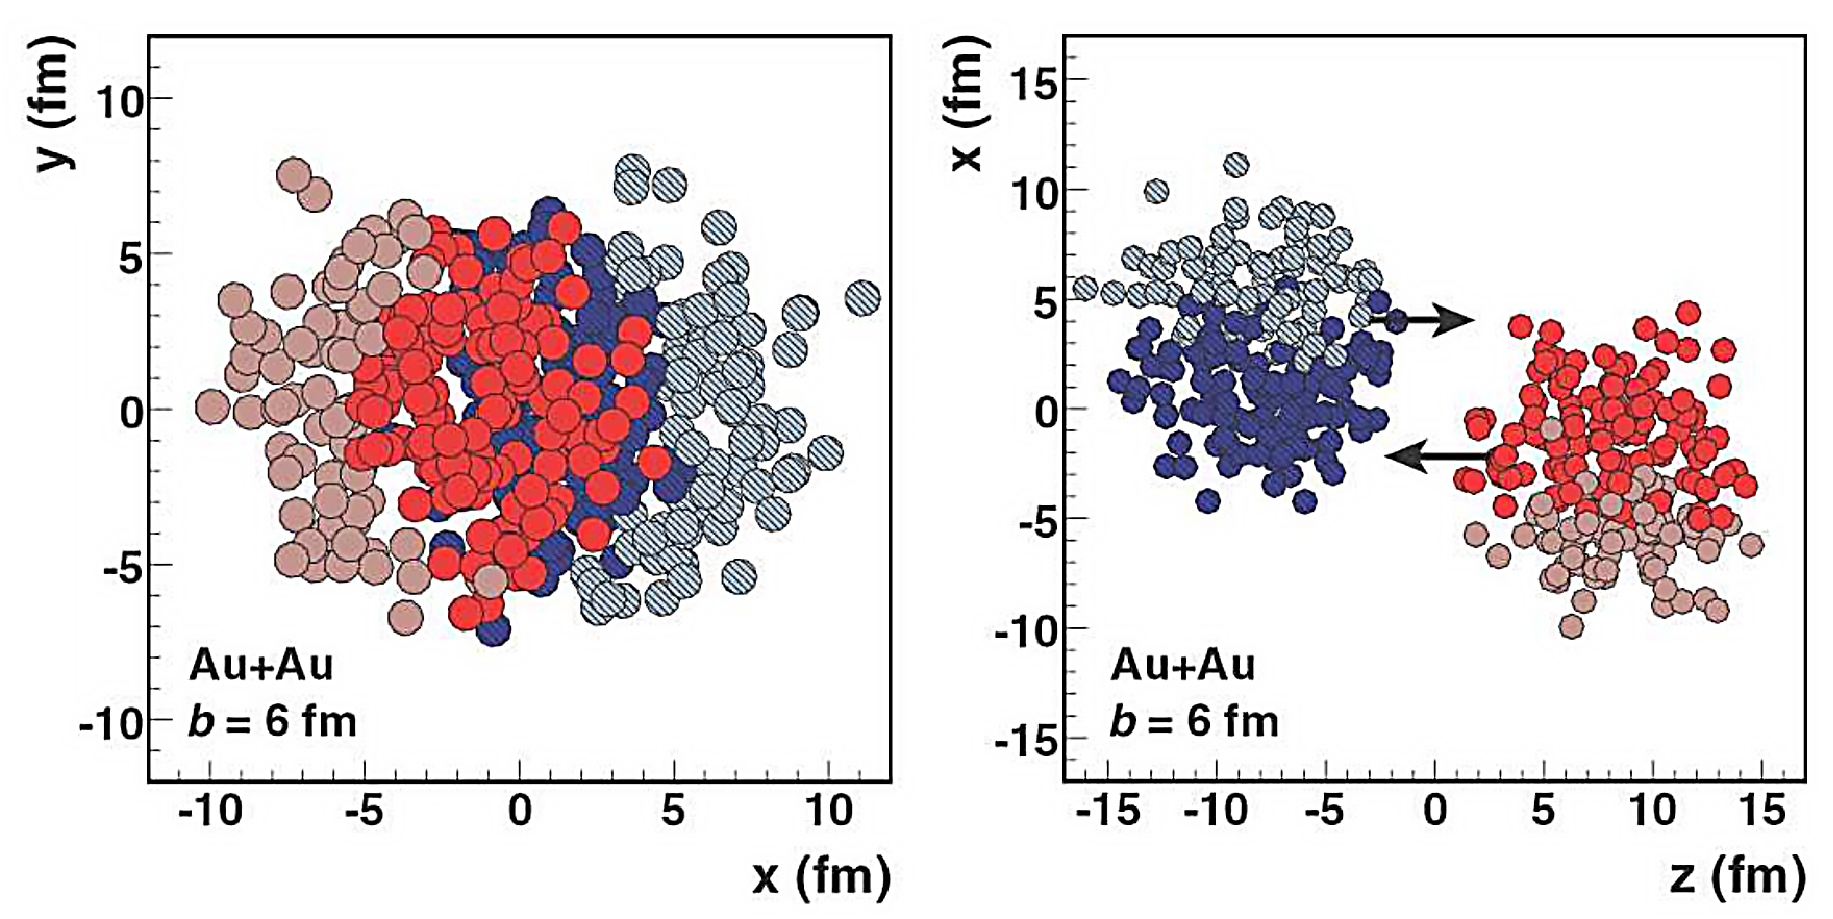
\includegraphics[width=0.9\linewidth]{Chapters/Analysis/Figs/glauber-pbpb.pdf}
\caption{Glauber Monte Carlo $Au-Au$ collision with impact parameter $b=6$ fm seen in the trasverse plane (left) and along the beam axis (right). Nucleons area is equal to $\sigma_{inel}^{NN}$. From \cite{Miller:2007ri}.}
\label{fig:GlauberAuAu}
\end{center}
\end{figure}

Through the Glauber model a measurement of the number of participant or spectator nucleons can provide an indirect measurement of the impact parameter of a nuclear collision.
Unfortunately neither $N_{part}(b)$ nor $N_{spec}(b)$ can be directly measured.
Typically the number of participants is related to the charged particles multiplicity ($N_{ch}$).
$N_{ch}$ has been measured over a large range of rapidity and is well described by a negative binomial distribution \cite{Aamodt:2009aa}.
This approach allows one to simulate an experimental multiplicity distribution that can then be linked to an experimental observable.
In figure \ref{fig:GlauberCent} the collision probability is represented as a function of $N_{ch}$. Additional axes represent the correlation between $N_{part}$, $b$ and fraction of the total cross section $\sigma/\sigma_{tot}$.
A typical centrality detector provides a signal whose amplitude is proportional to $N_{ch}$, hence the source of the main centrality evaluation.
An example is given in figure \ref{fig:GlauberVZERO}.


\begin{figure}[!t]
\begin{center}
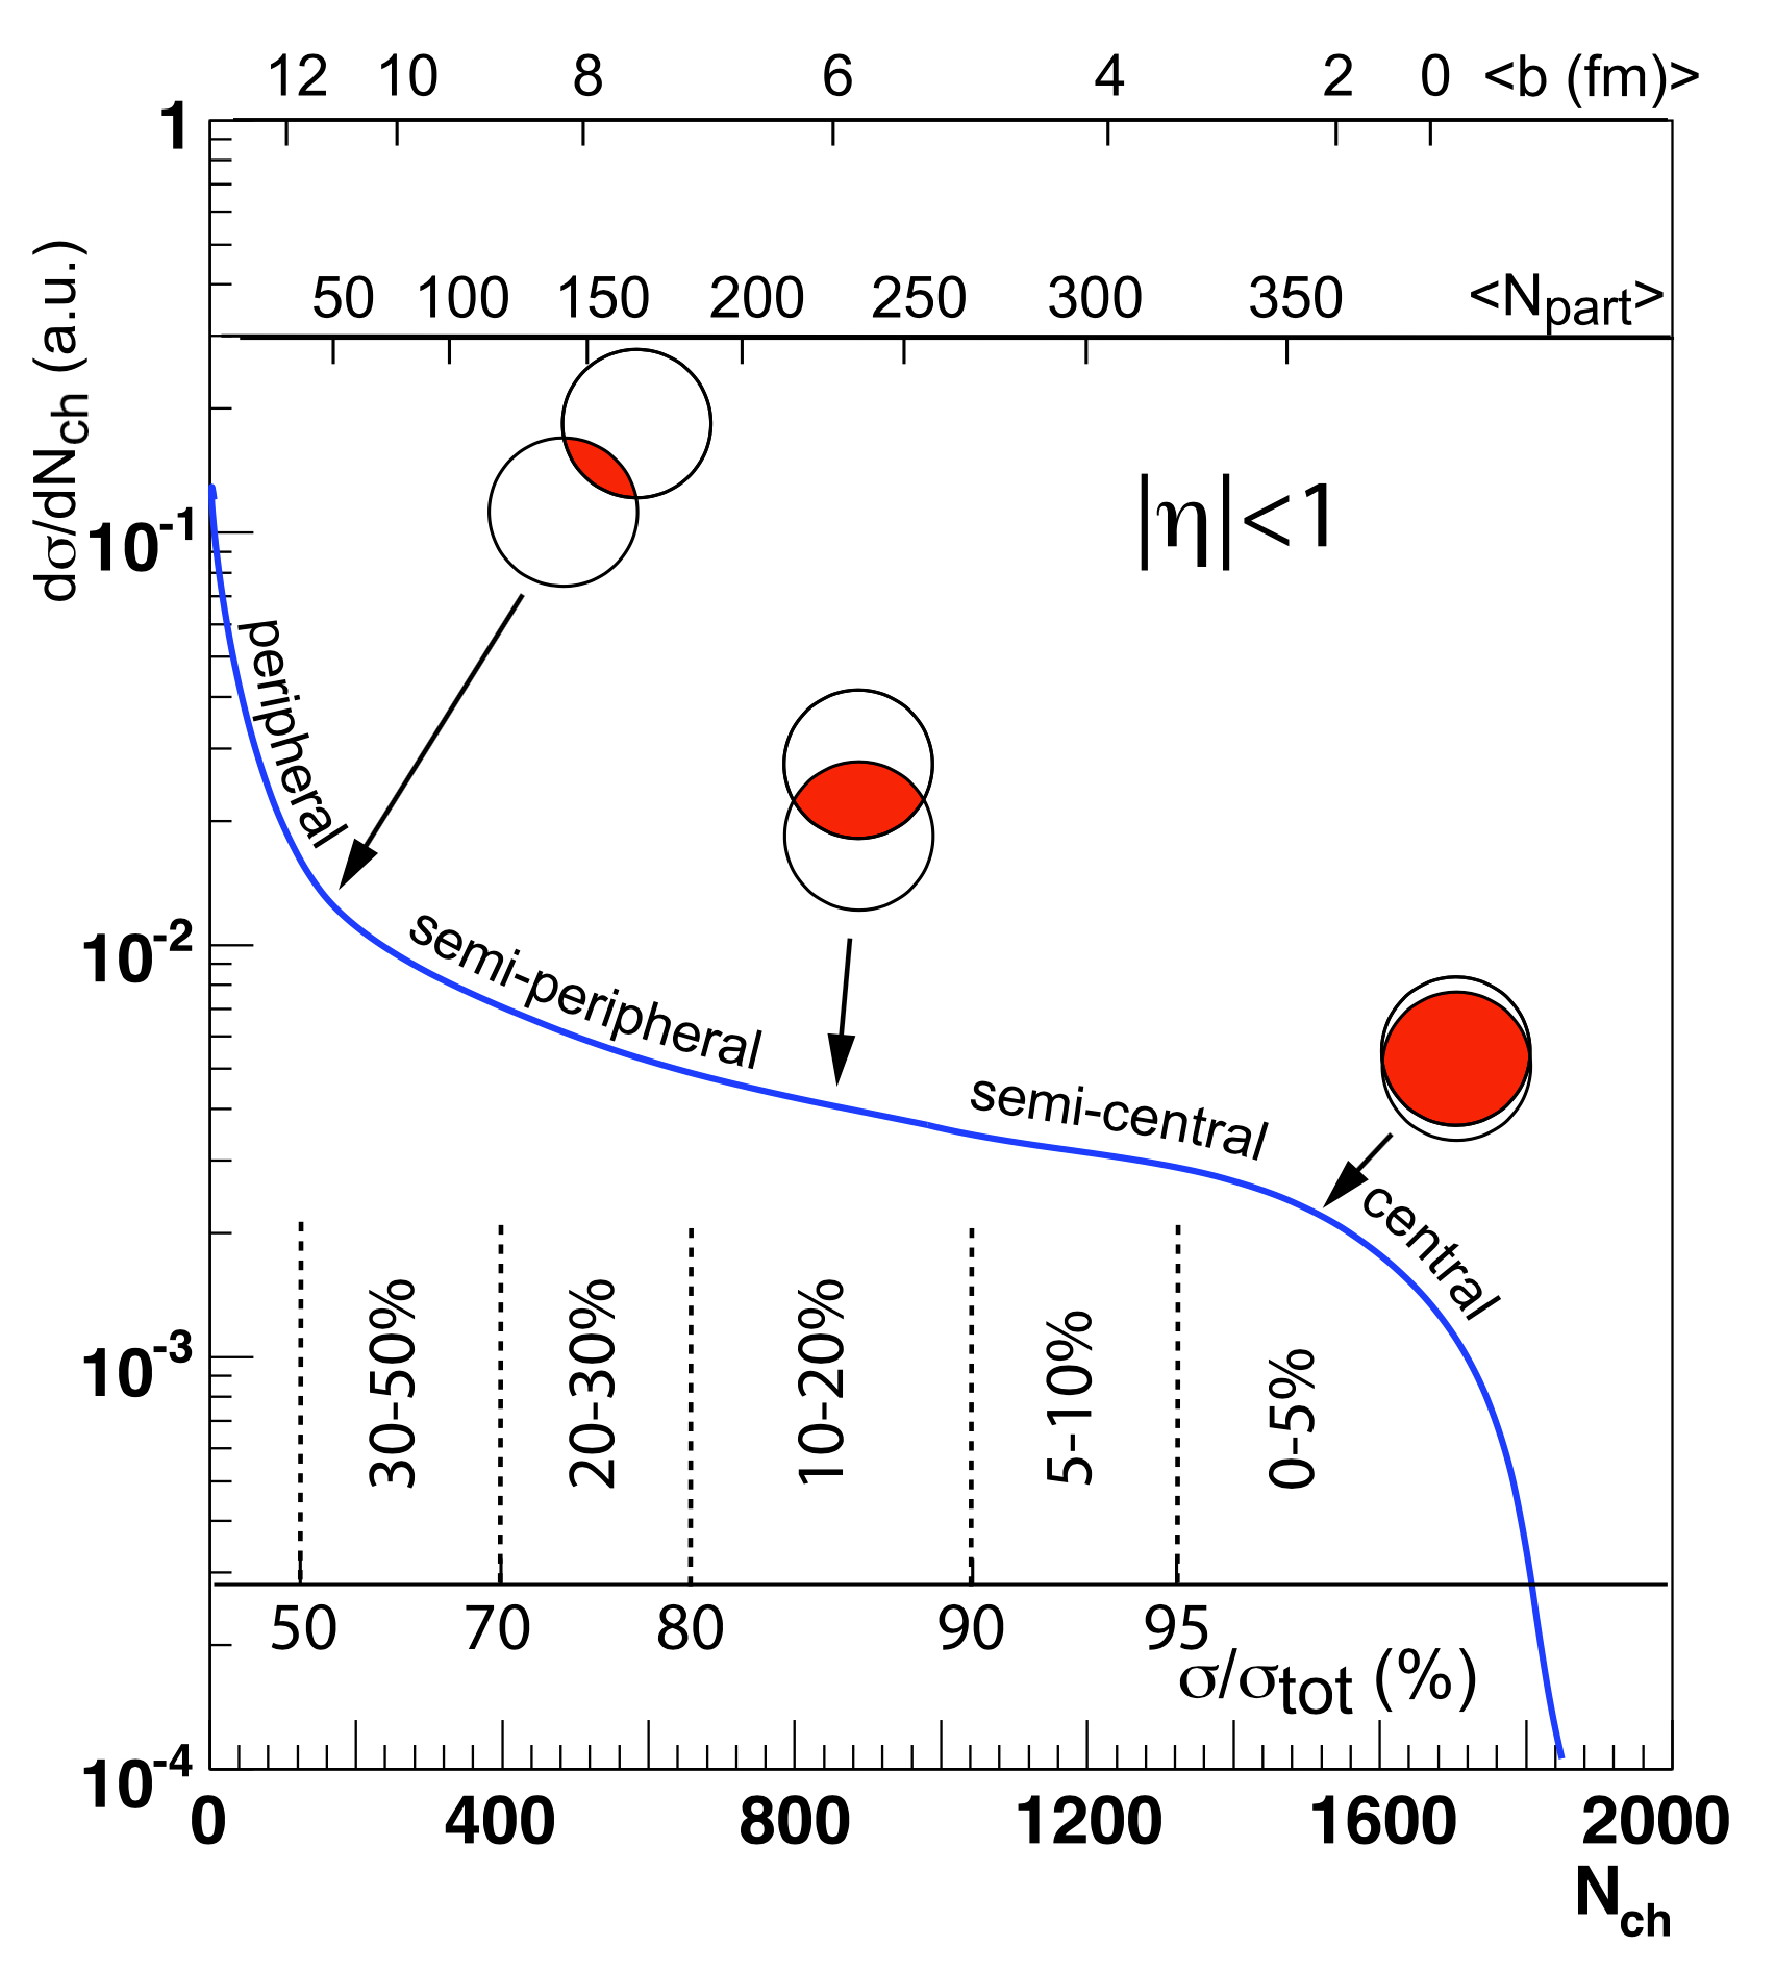
\includegraphics[width=0.75\linewidth]{Chapters/Analysis/Figs/glauber-centrality.pdf}
\caption{A cartoon example of the correlation of the final state observable $N_{ch}$ with Glauber calculated quantities ($b$, $N_{part}$). The plotted distribution and various values are illustrative and not actual measurements. From \cite{Miller:2007ri}.}
\label{fig:GlauberCent}
\end{center}
\end{figure}

\begin{figure}[!t]
\begin{center}
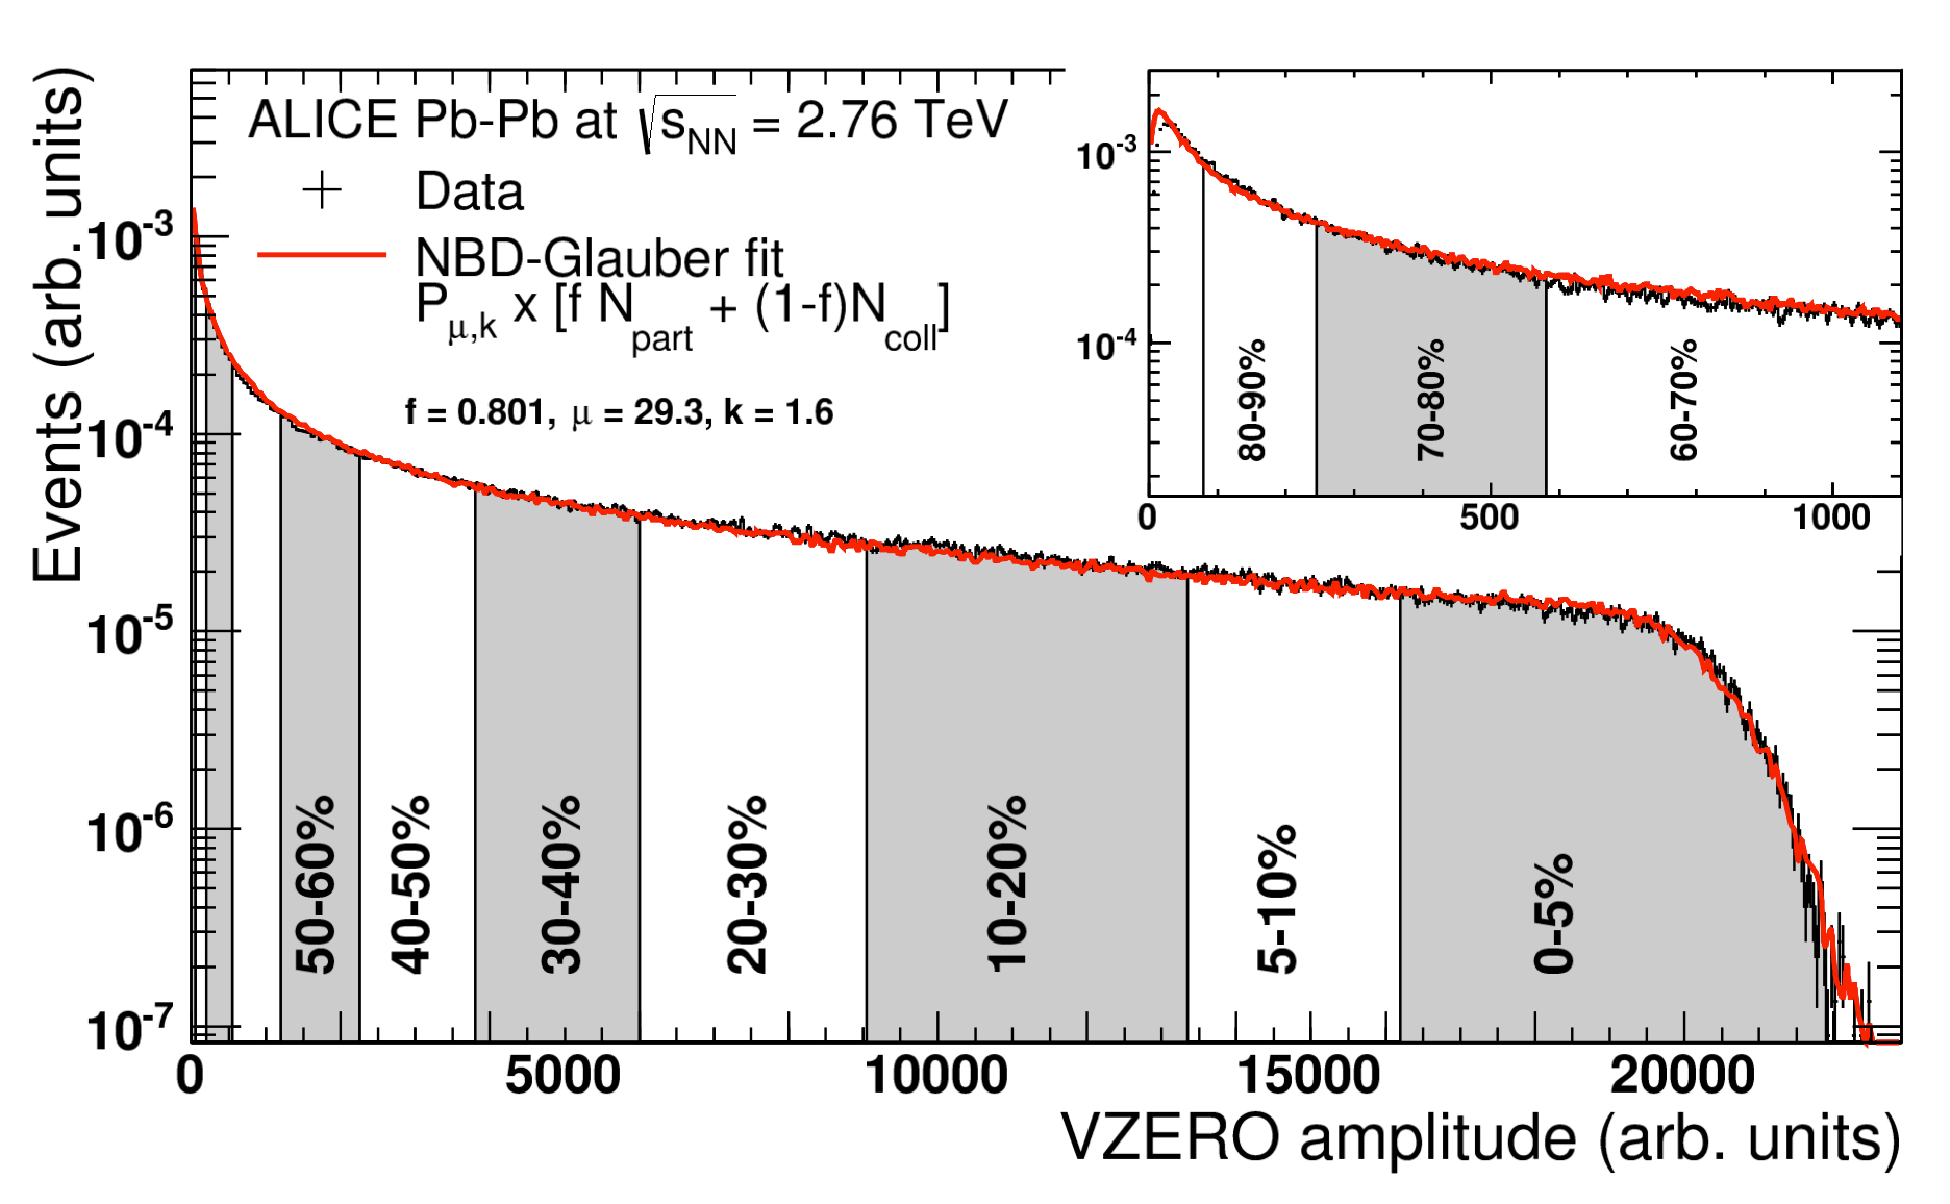
\includegraphics[width=0.85\linewidth]{Chapters/Analysis/Figs/glauber-vzero.pdf}
\caption{Distribution of the sum of signal amplitudes from a centrality detector. The distribution is fitted with the NBD-Glauber fit shown as a red line. The centrality classes used in the analysis are indicated in the figure. The inset shows a zoom of the most peripheral region. From \cite{Abelev:2013qoq}.}
\label{fig:GlauberVZERO}
\end{center}
\end{figure}

\subsection{Nuclear modification factor}\label{RAA}
In general the study of the modifications of the production of hard probes in heavy nuclei collisions, with respect to proton--proton collisions, makes use of the nuclear modification factor which is defined as:

\begin{equation}
\label{eq:RAA}
R_{\rm{AA}}^X = \frac{N_{\rm{AA}}^X}{<N_{coll}>\cdot N_{\rm{pp}}^X}
\end{equation}

where $<N_{coll}>$ is the average number of binary nucleon--nucleon collisions happening in the nucleus--nucleus collision and $N_{\rm{pp}}^X$ and $N_{\rm{AA}}^X$ are the yields of $X$ states in a proton--proton and a nucleus--nucleus collision, respectively.
The denominator of this expression originates from the assumption that a nuclear collision is an incoherent superposition of nucleon collisions.
To simplify, the denominator corresponds to the number of $X$s one would be able to measure in the case of absence of nuclear effects.
% It is also assumed that during each binary collision the spectator nucleons are neither participating nor perturbing the binary collision outcome.
The $R_{\rm{AA}}^X$ represents the deviation from the picture in which the nucleus collision is an incoherent scattering of its nucleon constituents
The yields of a given state X are defined as the ratio between its production cross section and the minimum bias cross section:

% \begin{equation}
% \label{eq:yields}
% N^X_{\rm{pp}} = \frac{\sigma^X_{\rm{pp}}}{\sigma^{MB}_{\rm{pp}}}
% \end{equation}

Since the nuclear overlap function is defined by:

\begin{equation}
\label{eq:TAA}
T_{\rm{AA}} = \frac{<N_{coll}>}{\sigma_{\rm{pp}_{MB}}}
\end{equation}
Equation \ref{eq:RAA} can be written as:

\begin{equation}
\label{eq:RAA2}
R_{\rm{AA}}^X = \frac{N_{\rm{AA}}^X}{T_{\rm{AA}} \cdot \sigma_{\rm{pp}}^X}
\end{equation}
Three scenarios can be foreseen for the nuclear modification factor:
\begin{itemize}
\item $R_{\rm{AA}}^X<1$: a net suppression of the production of $X$s is measured;
\item $R_{\rm{AA}}^X>1$: a net enhancement of the production of $X$s is observed; 
\item $R_{\rm{AA}}^X=1$: the nucleus--nucleus collision can be interpreted as an incoherent superposition of binary nucleon--nucleon collisions. Note that this situation might occur even in the case where suppression and enhancement effects balance out perfectly.
\end{itemize}

\section{Bottomonium study}
\subsection{Rationale of bottomonium study} %Section - 3.1
% A detailed study of the properties of the Quark-Gluon Plasma (QGP)~\cite{Shuryak:1978ij} is the main goal of heavy-ion experiments at ultra-relativistic energies~\cite{Adams:2005dq,Muller:2012zq}.
% ALICE joins the efforts of the previous generation of similar experiments, extending the reach of such studies.

Quarkonia, $i.e.$ bound states of charm or bottom quark-antiquark pairs, are sensitive probes of color deconfinement. 
Due to their heavy mass, heavy quarks are produced in the initial parton--parton interactions and propagate in the hot and dense medium.
The presence of the medium provides a screening between the colour charges of the quarks and anti-quarks in a way which is analogous to the Debye screening of electric charges in a plasma, eventually leading to the dissociation of the bound states \cite{Matsui:1986dk,Brambilla:2010cs,Andronic:2015wma}.
The dissociation temperature depends on the binding energy of the quarkonium states ~\cite{Digal:2001ue}. 
% If this dissociation process happens only part of the total production of a given quarkonium state will emerge from the QGP region.
Less bound states are easily melted, while the most bound states required a much higher temperature.
The dissolution of energetically ordered resonances, and their resulting suppression in the final state, can be correlated to the medium temperature.
This melting process, called sequential suppression, can therefore be used as a thermometer of the medium itself (see figure \ref{fig:QGP_thermo}).

First studies of quarkonium production in heavy-ion collisions were devoted to charmonium states, and a suppression of their yields was observed at the SPS~\cite{abreu:in2p3-00002434,Alessandro:2004ap,Arnaldi:2007zz}, at RHIC~\cite{Adare:2011yf,Abelev:2009qaa} and at the LHC~\cite{Abelev:2012rv,Chatrchyan:2012np,Adam:2016rdg}. 
The much smaller \jpsi suppression observed at LHC energies, despite the centre-of-mass energy per nucleon pair (\snn) being one order of magnitude larger than at RHIC, is now explained by means of a competition between suppression and regeneration phenomena, which occurs during the deconfined phase and/or at the hadronization stage of the system~\cite{BraunMunzinger:2000px,Thews:2000rj,Zhao:2011cv,Zhou:2014kka}.
% In general free quarks and anti-quarks of the same species may form a quarkonium bound state.
At the LHC energies, the high abundance of charm quarks and bottom quarks to some extent makes non-negligible the probability of the regeneration to occur.
While at RHIC the charm pairs abundance was of about $10$ pairs per central collision, at the LHC the estimation rises to $\simeq100$.
The recombination process can lead to an enhancement of the production of a given quarkonium state, providing a concurrent effect to the aforementioned suppression and has been found to be more important at low $p_{\rm T}$ (due to easier recombination at low momenta) and in the most central collisions (due to the larger number of $c\overline{c}$ pairs) \cite{Abelev:2013ila,Adam:2015isa}.

Models able to reproduce the charmonium production rates include a sizeable regeneration contribution.
However, the details of the suppression and regeneration mechanisms cannot be fully disentangled when measuring only charmonium states.
Bottomonium states are expected to be much less affected by recombination with respect to charmonium states, due to the higher mass of the bottom quarks, hence to their lower abundance in the system.
Since the  ${\rm b{\overline b}}$ yield in central heavy-ion collisions amount to a few pairs ($\approx 10$) per event at the LHC, the probability for regeneration of bottomonia through recombination is much smaller than in the case of charmonia ($\approx 100$ pairs).
Incidentally the average number of ${\rm b{\overline b}}$ pairs at the LHC is similar to the abundance of $c\bar{c}$ pairs at RHIC.
The much lower regeneration contribution makes the bottomonium states the best candidates for a Debye-based QGP thermometer.

% The separation of suppression and regeneration mechanisms' effects is a puzzling task.
% Models able to reproduce the charmonium states production rates include a regeneration contribution.
% The abundances of charm and anti-charm quarks, at the LHC collision conditions, make the regeneration contribution important.
% Decoupling of the concurrent effects using measurements on the charmonium states appears to be not trivial.
% Is however worth mentioning that bottom quarks pairs abundance at the LHC is expected to be similar to the charm pairs abundance at RHIC, hence the recombination effect should be negligible for the bottomonium states.
% bottomonium states are expected to be much less affected by recombination with respect to charmonium states, due to the higher mass of the bottom quarks, hence to their lower abundance.
% Since the  ${\rm b{\overline b}}$ yield in central heavy-ion collisions amount to a few pairs ($\approx 10$) per event at the LHC, the probability for regeneration of bottomonia through recombination is much smaller than in the case of charmonia ($\approx 100$ pairs).


\begin{figure}[!t]
\begin{center}
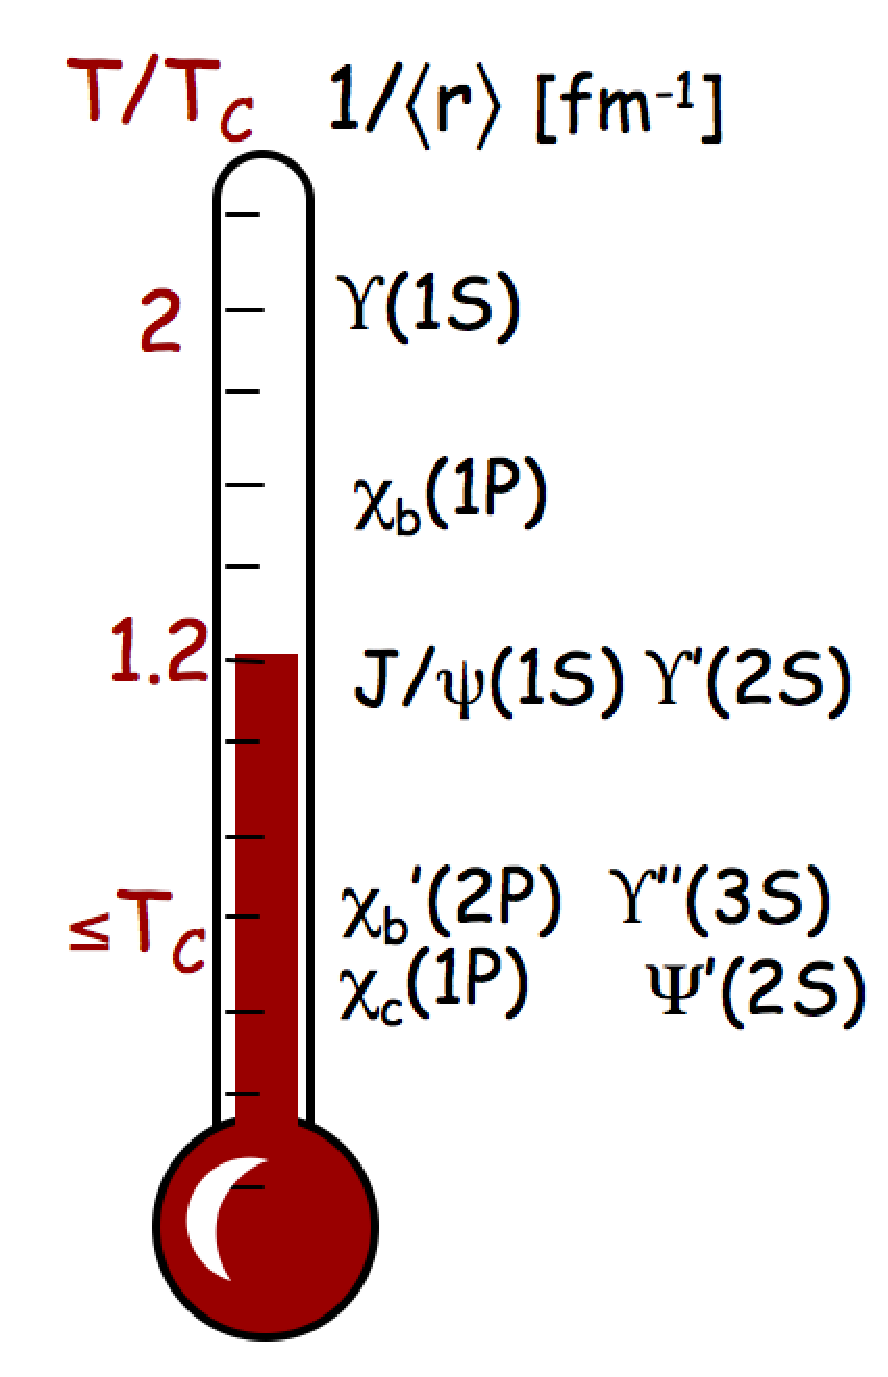
\includegraphics[width=0.3\linewidth]{Chapters/Introduction/Figs/thermometer.pdf}
\caption{Cartoon representation of the dissociation temperatures of several quarkonium states. The sequential suppression can provide information regarding the average kinetic energy of the formed QGP droplet, leading to a QGP thermometer.}
From \cite{Mocsy:2008eg}
\label{fig:QGP_thermo}
\end{center}
\end{figure}

Is worth mentioning that, for bottomonium production, perturbative calculations of production rates in elementary nucleon-nucleon collisions are more reliable than for charmonium yields due to the higher mass of the bottom quark with respect to charm. 

In conclusion the study of bottomonium production can provide an independent measurement of QGP characteristics, adding up to charmonium measurements to better understand the dissociation and recombination contributions to quarkonia production.

% \subsection{Complexity of bottomonium study}
% Due to the higher mass of the constituting quarks, the abundance of bottomonium states in the final state of QGP evolution is much lower if compared to those of charmonium states.
% This physical characteristic limits the available statistics.
In addition bottomonium production theoretical estimates \cite{Krouppa:2015yoa} indicate that its formation may occur before QGP thermalization \cite{Mauricio:2007vz}. 
In this situation, a quantitative description of the influence of the medium on the bound states becomes challenging.
Even if the dissociation temperatures may vary significantly between different models \cite{Brambilla:2010cs,Andronic:2015wma}, it is commonly accepted \cite{Burnier:2014ssa} that the spectral functions of the bottomonium states are affected by the high temperature of the surrounding medium.
This effect leads to much larger spectral widths than in vacuum.
% Finally, even if the regeneration of bottomonium can be considered negligible at LHC energies, another effect partly disrupts the possibility to use bottomonium states as a QGP thermometer.
% In fact, taking into account that feed-down processes from higher-mass resonances  are not negligible (around 40\% for the \upsis and 30\% for the \upsiss \cite{Andronic:2015wma}), the evaluation of the medium temperature via bottomonium measurements remains a complex endeavour.
Finally, the feed-down processes from higher mass resonances are not negligible (around 40\% for the \upsis and 30\% for the \upsiss \cite{Andronic:2015wma}) and must be therefore taken into account in the study of the suppression of the ground states.

The bottomonium suppression due to the QGP should be disentangled from the modification due to Cold Nuclear Matter (CNM) effects, such as the nuclear modification of the parton distribution functions \cite{Eskola:1998df,Eskola:2009uj}, as well as parton energy loss \cite{Arleo:2012rs}.
These effects on the bottomonium production were studied in \ppb collisions by ALICE \cite{Abelev:2014oea} and LHCb \cite{Aaij:2014mza}, which reported for the \upsis a nuclear modification factor slightly lower than unity at forward rapidity and compatible with unity at backward rapidity, although with significant uncertainties (see Fig. \ref{fig:ALICE_pPb_jpsi_upsi}).
As a side note, in both rapidity ranges the compatibility between $J/\psi$ and \upsis is verified, suggesting a similar CNM effects contribution for charmonium and bottomonium.

\begin{figure}[!t]
\begin{center}
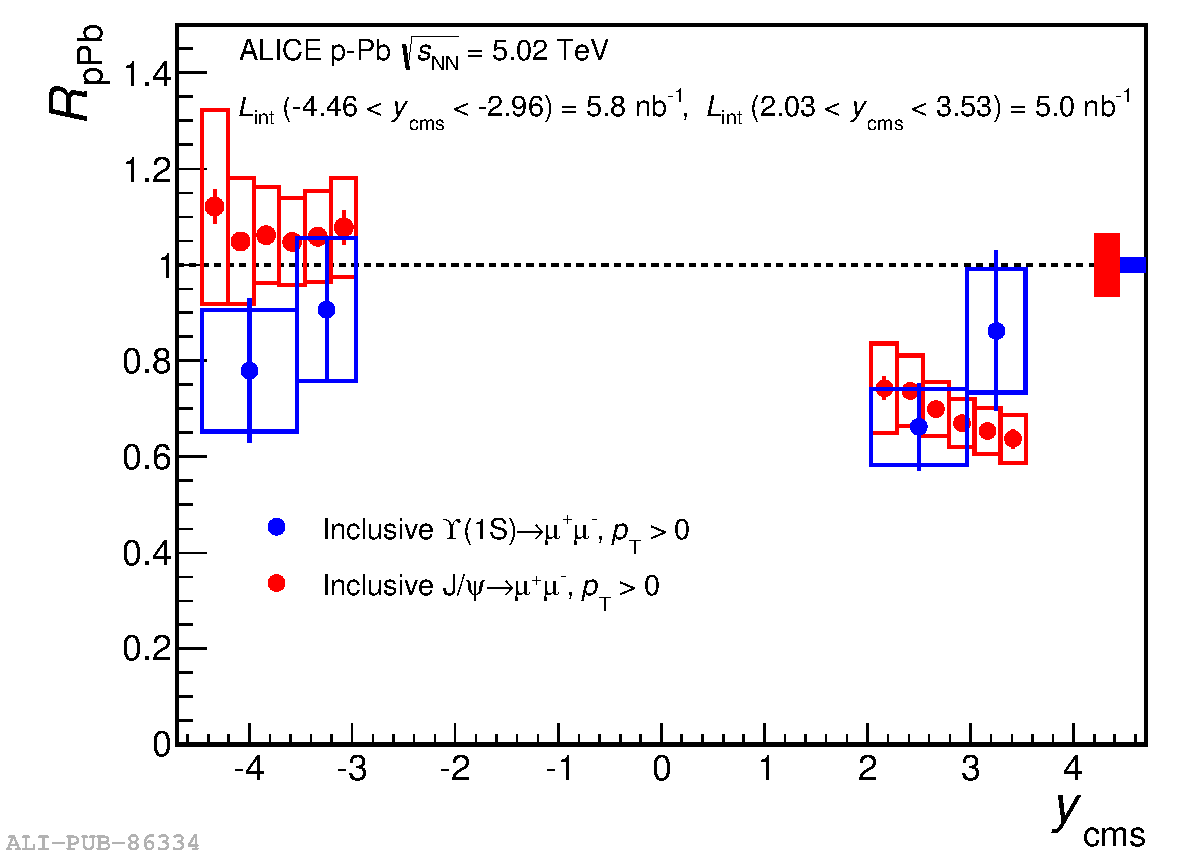
\includegraphics[width=0.8\linewidth]{Chapters/Analysis/Figs/2014-Oct-08-RpPb_Ups_Jpsi_b.pdf}
\caption{$J/\psi$ (red) and \upsis (blue) nuclear modification factor as a function of $y$ measured by ALICE in p-Pb collisions ($-4.46<y<-2.96$ and $2.03<y<3.53$) at $\sqrt{s_{_{\rm NN}}}=5.02$ TeV. From \cite{Caffarri:2016xvd}}
\label{fig:ALICE_pPb_jpsi_upsi}
\end{center}
\end{figure}

% $p-Pb$ collisions are the CNM baseline since the achieved energy density is not enough to cause QGP production, but the nucleons of the colliding nuclei might be perturbed by the others.
Recently, ATLAS results indicate a significant suppression of the \upsis around mid-rapidity~\cite{Aaboud:2017cif}.  
Additional measurements at forward/backward rapidity with higher statistics, are needed to fully constrain the models.

\begin{figure}[!t]
\begin{center}
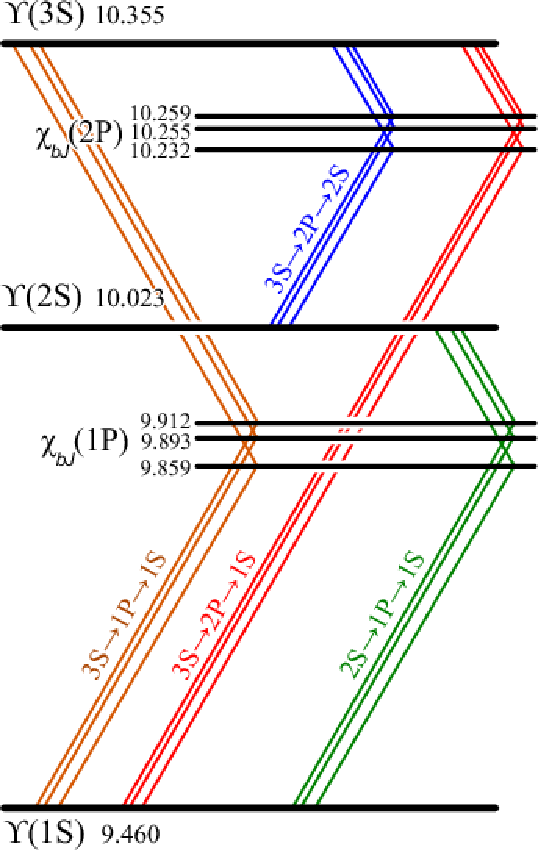
\includegraphics[width=0.45\linewidth]{Chapters/Analysis/Figs/BottomoniumSpectro.pdf}
\caption{Representation of possible feed-down patterns for bottomonium states as measured from BaBar collaboration and reported in \cite{Lees:2014qea}. The numbers refer to the masses as reported by the PDG. Splittings in the photon spectra for these cascades are due to the mass splittings in the intermediate states $\chi_{bJ}$ with J = 0, 1 or 2. From \cite{Lees:2014qea}}
\label{fig:BBSpectro}
\end{center}
\end{figure}

\subsection{Previous results}

The charmonium production was measured in heavy-ion collisions at the SPS and RHIC. 
A similar suppression with respect to the yields measured in pp collisions was observed in the two cases, despite the large gap in the colliding energy \cite{Rapp:2017chc}.
Before the beginning of the LHC operations, the RHIC accelerator was leading the edge of QGP-oriented research.
The PHENIX collaboration measured the $J/\psi$ suppression in Au-Au collisions at $\sqrt{s_{_{\rm NN}}}=200$ GeV, highlighting a suppression strongly correlated with the centrality of the collision.
% Since the operations of RHIC the measured a suppression appeared similar to the SPS one, despite the latter had much higher colliding energy.
The first $J/\psi$ measurements at the LHC challenged even more the commonly accepted models, since a much lower suppression was observed in the most central collisions at LHC at $\sqrt{s_{_{\rm NN}}}=2.76$ TeV with respect to what had been observed at $\sqrt{s_{_{\rm NN}}}=200$ GeV at RHIC (Fig. \ref{fig:LHC_RHIC_jpsi}).

\begin{figure}[!t]
\begin{center}
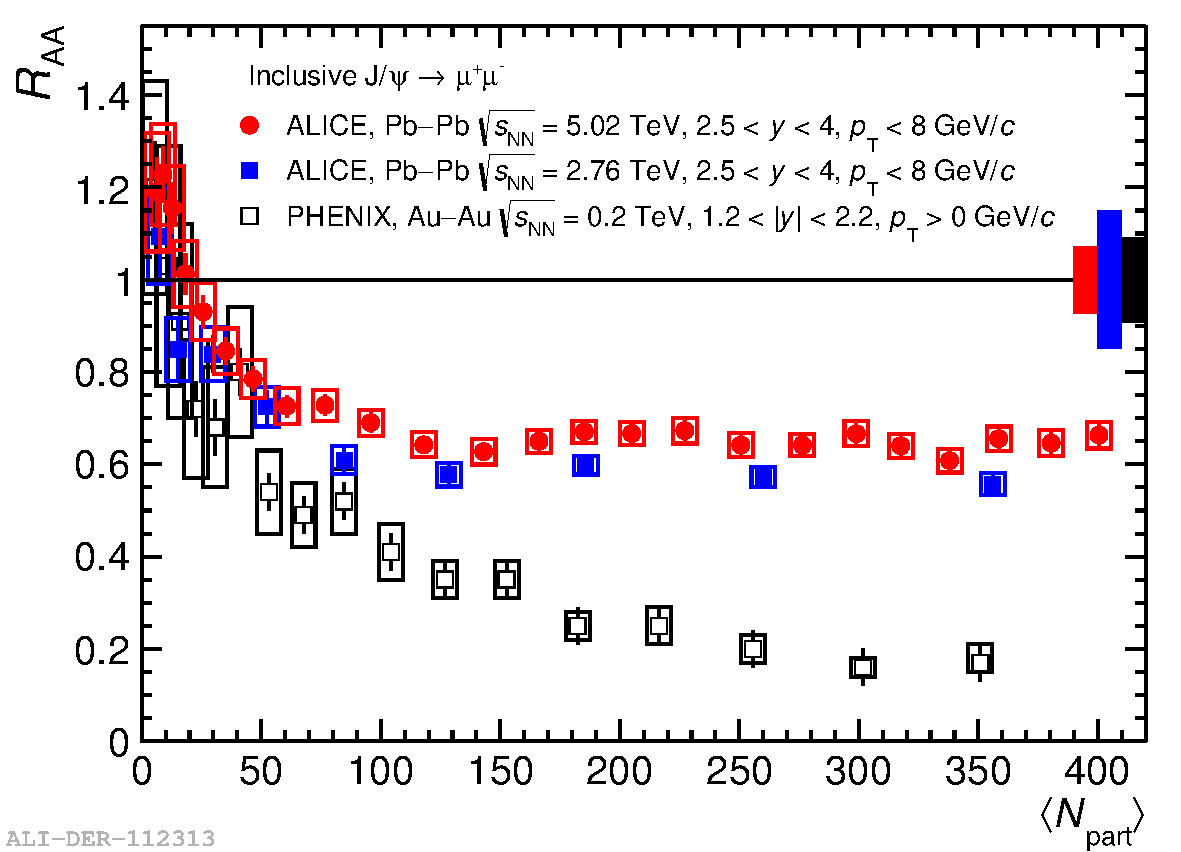
\includegraphics[width=0.8\linewidth]{Chapters/Analysis/Figs/2016-Sep-15-RAA_centr_Alice5_Alice276_Phenix.pdf}
\caption{$J/\psi$ nuclear modification factor measured by PHENIX (RHIC) at $\sqrt{s_{_{\rm NN}}}=200$ GeV (open black) and by ALICE at the LHC at $\sqrt{s_{_{\rm NN}}}=2.76$ and $5.02$ TeV (blue and red, respectively), as a function of the number of participant nucleons. The RHIC points appear systematically below ALICE ones for $<N_{part}>=50$, indicating a much lower suppression at LHC in the most central collisions. The two ALICE series appear to be in agreement over the whole centrality spectrum despite a factor ~$\times2$ in the center of mass energy. From \cite{Caffarri:2016xvd}}
\label{fig:LHC_RHIC_jpsi}
\end{center}
\end{figure}

\begin{figure}[!t]
\begin{center}
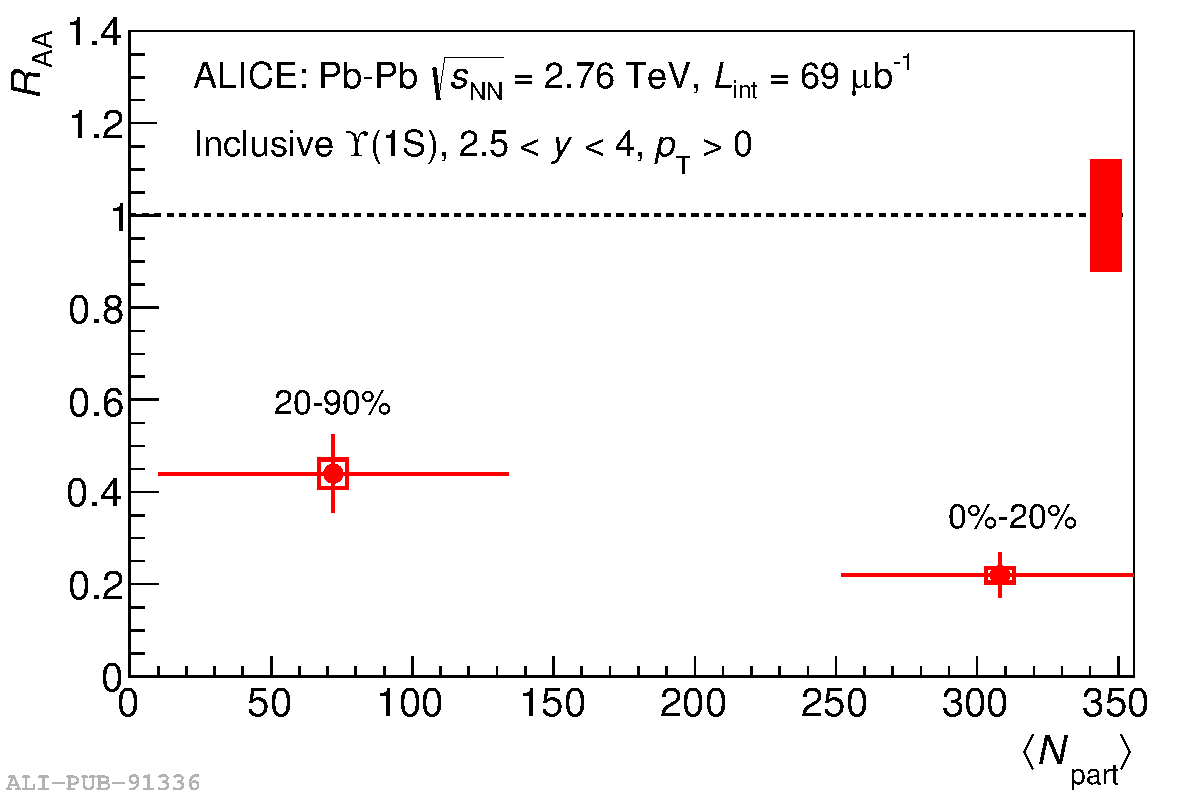
\includegraphics[width=0.8\linewidth]{Chapters/Analysis/Figs/2014-Dec-16-Raa_centr.pdf}
\caption{\upsi nuclear modification factor measured at the LHC by ALICE at $\sqrt{s_{_{\rm NN}}}=2.76$ TeV. Two centrality bins are shown, referring to the quoted centrality distribution percentiles. From \cite{Abelev:2014nua}}
\label{fig:LHC_upsi}
\end{center}
\end{figure}

The data can be consistently described by models that implement statistical regeneration mechanisms for the $J/\psi$ production.
Such models suggested that for \upsis production the regeneration effects would be negligible, even at LHC energies conditions, hence the bottomonium production studies were performed as well on the same data set.
As one can notice by performing a comparison between figures \ref{fig:LHC_RHIC_jpsi} and \ref{fig:LHC_upsi} the \upsi $R_{\rm{AA}}$ at $\sqrt{s_{_{\rm NN}}}=2.76$ TeV appears to be similar to the $J/\psi$ one, measured at RHIC.
This observation can be related to the fact that the estimations of the total number of bottom quark pairs at the LHC is similar to the number of charm quark pairs at RHIC, even if different medium temperatures and feed-down fractions could alter the picture.
A strong suppression of the \upsis state in \pbpb collisions at $\sqrt{s_{_{\rm NN}}}=2.76$ TeV was measured by ALICE using properly scaled measurements from pp collisions by ALICE \cite{Abelev:2014nua} and CMS \cite{Chatrchyan:2012lxa,Khachatryan:2016xxp}, in the rapidity ranges $2.5<y<4.0$ and $|y|<2.4$, respectively (see Fig. \ref{fig:ALICE_CMS_upsi}). 

\begin{figure}[!t]
\begin{center}
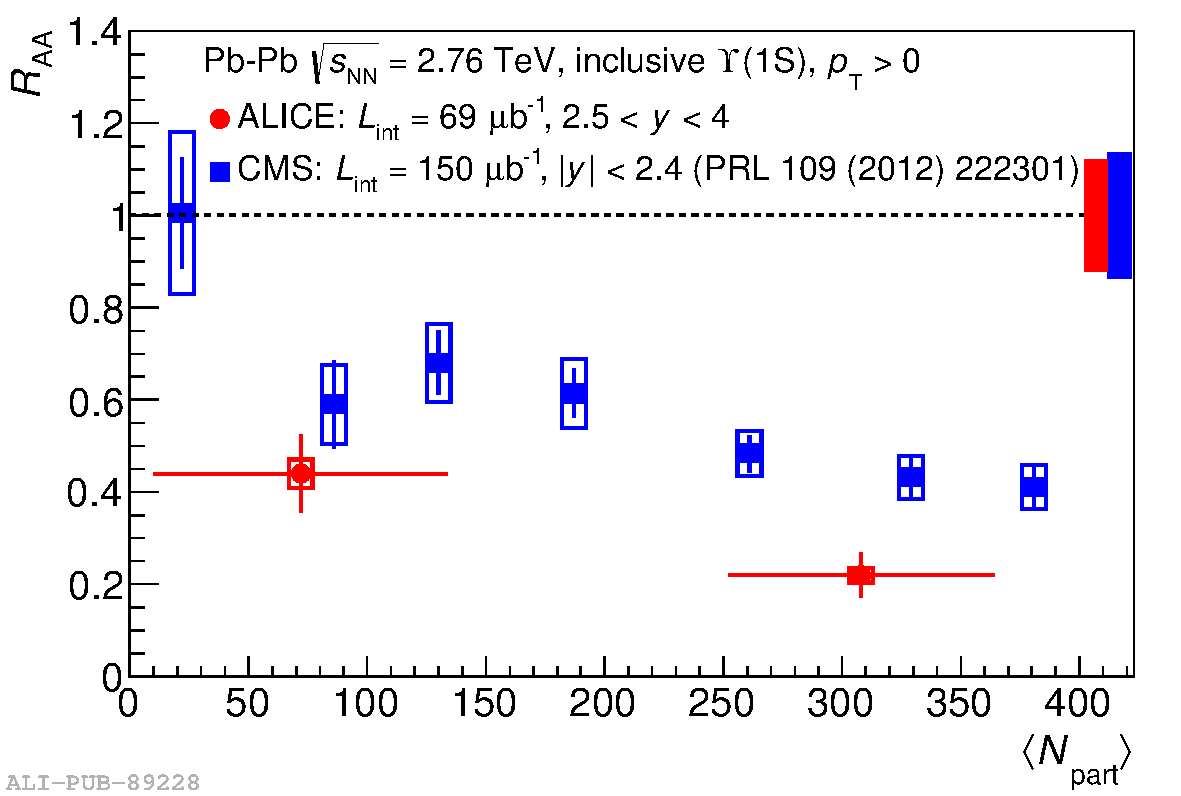
\includegraphics[width=0.47\linewidth]{Chapters/Analysis/Figs/2014-Nov-05-Raa_CMS_centr.pdf}
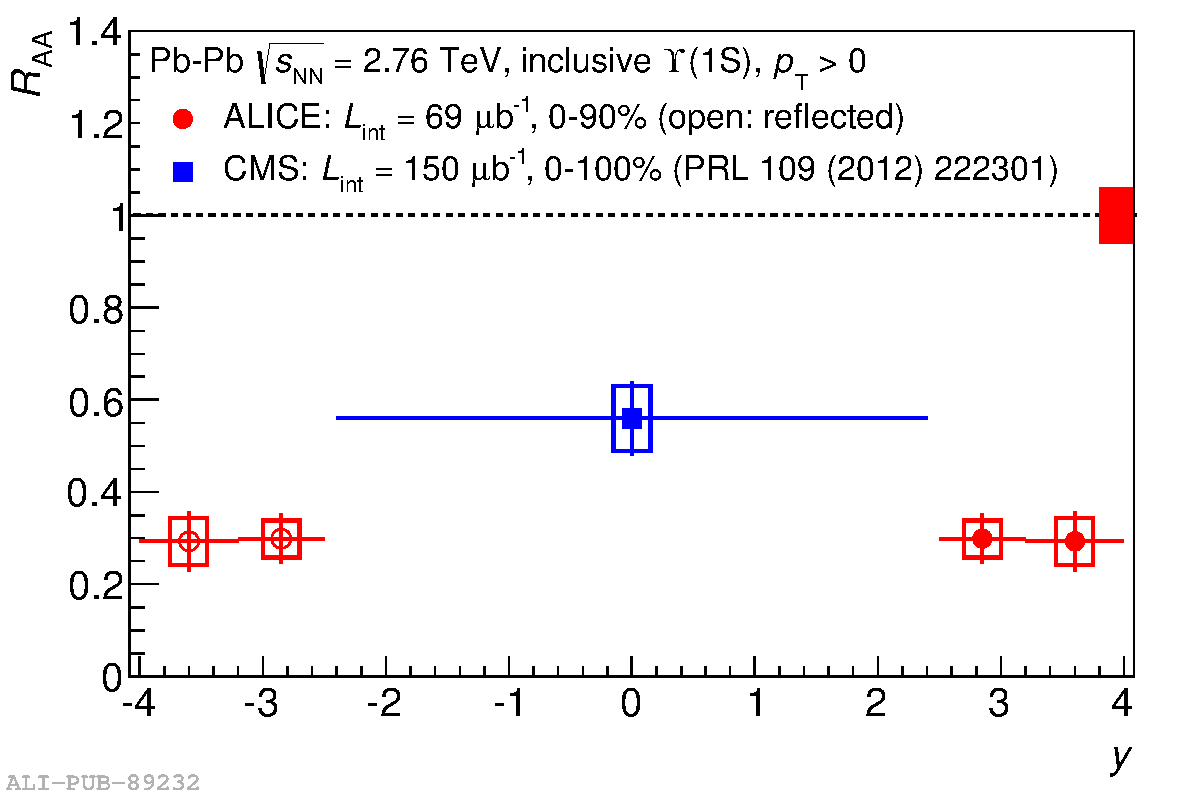
\includegraphics[width=0.47\linewidth]{Chapters/Analysis/Figs/2014-Nov-05-Raa_CMS_rap.pdf}
\caption{\upsis nuclear modification factor as a function of $<N_{part}>$ (left) and $y$ (right) measured by ALICE (red points, $2.5<y<4.0$) and CMS (blue points, $|y|<2.4$) at $\sqrt{s_{_{\rm NN}}}=2.76$ TeV. From \cite{Abelev:2014nua}}
\label{fig:ALICE_CMS_upsi}
\end{center}
\end{figure}

The suppression increases with the centrality of the collision, reaching about 60\% and 80\% for the most central collisions at mid-~\cite{Khachatryan:2016xxp} and forward rapidity~\cite{Abelev:2014nua}, respectively. 
Moreover, the \upsiss suppression reaches about 90\% while the one for \upsisss is compatible with 100\% \cite{Khachatryan:2016xxp}. 
The transverse momentum dependence of the \upsis \raa, measured for $p_{\rm T}<20$ GeV/c by CMS~\cite{Khachatryan:2016xxp}, is compatible with a constant value. 
When considering the $y$-dependence resulting from the comparison of ALICE and CMS results, there is an indication for a stronger suppression at forward $y$.
Transport models \cite{Zhou:2014kka,Du:2017qkv} fairly reproduce the experimental observations of CMS, while they tend to overestimate the $R_{\rm AA}$ values measured by ALICE. 
Similar conclusions can be obtained in the frame of an anisotropic hydrodynamic model \cite{Krouppa:2017jlg}. 
The comparison between $J/\psi$ and \upsis measurements performed by ALICE, reported in figure \ref{fig:ALICE_jpsi_upsi}, denotes a much stronger suppression for the latter ($>3\sigma$) in the most central collisions.

\begin{figure}[!t]
\begin{center}
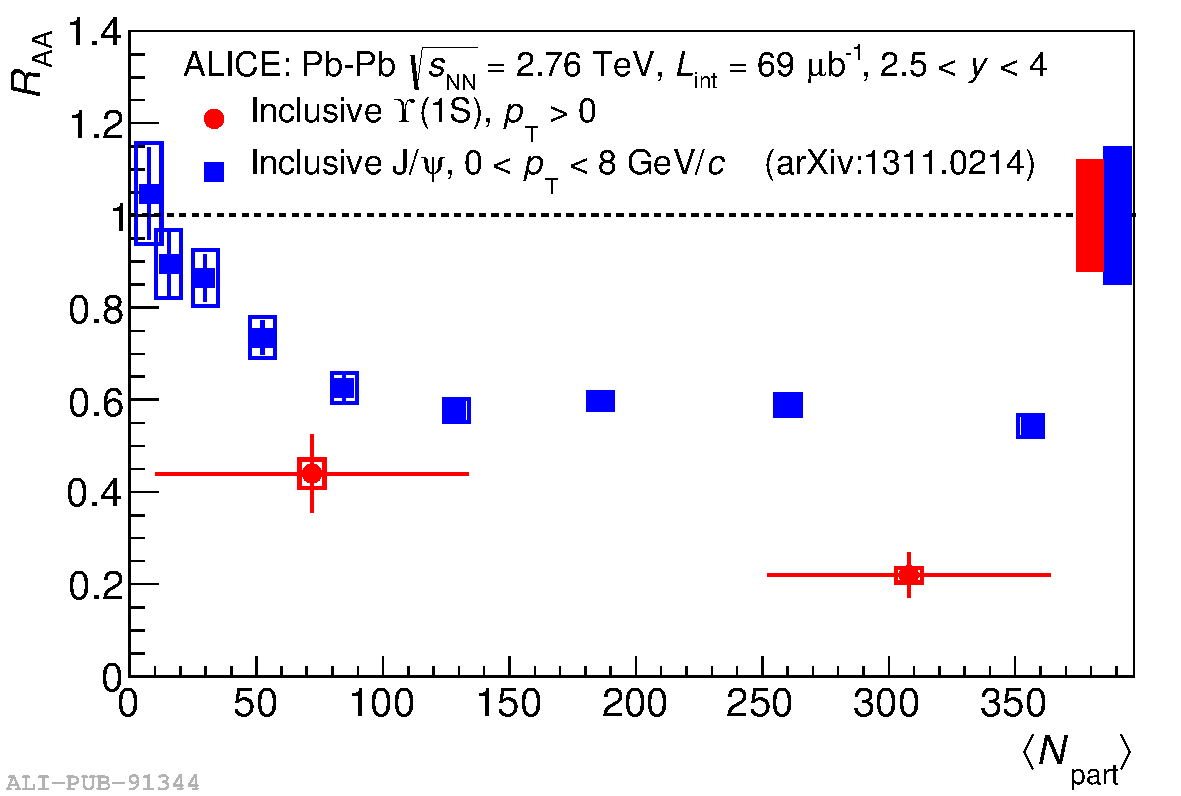
\includegraphics[width=0.8\linewidth]{Chapters/Analysis/Figs/2014-Dec-16-Raa_Jpsi_centr.pdf}
\caption{$J/\psi$ (blue) and \upsis (red) nuclear modification factor as a function of $<N_{part}>$ measured by ALICE at forward rapidity ($2.5<y<4.0$) at $\sqrt{s_{_{\rm NN}}}=2.76$ \rm{TeV}. From \cite{Abelev:2014nua}}
\label{fig:ALICE_jpsi_upsi}
\end{center}
\end{figure}

% The bottomonium suppression due to the QGP should be disentangled from the suppression due to Cold Nuclear Matter (CNM) effects, such as the nuclear modification of the parton distribution functions \cite{Eskola:1998df,Eskola:2009uj}, as well as parton energy loss \cite{Arleo:2012rs}.
% These effects on the bottomonium production were studied in \ppb collisions by ALICE \cite{Abelev:2014oea} and LHCb \cite{Aaij:2014mza}, which reported for the \upsis a nuclear modification factor slightly lower than unity at forward rapidity and compatible with unity at backward rapidity, although with significant uncertainties (see Fig. \ref{fig:ALICE_pPb_jpsi_upsi}).
% As a side note, in both rapidity ranges the compatibility between $J/\psi$ and \upsis is verified, suggesting a similar CNM effects contribution for charmonium and bottomonium.

% \begin{figure}[!t]
% \begin{center}
% 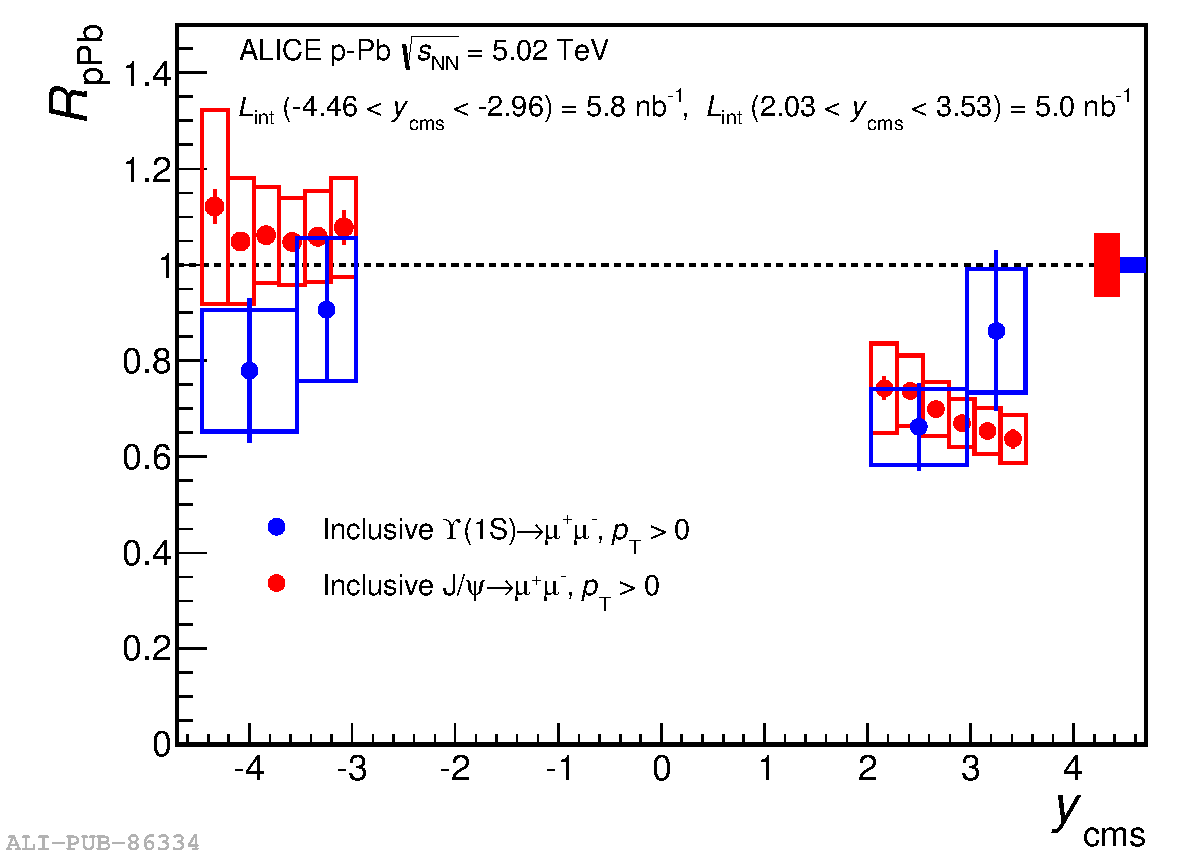
\includegraphics[width=0.8\linewidth]{Chapters/Analysis/Figs/2014-Oct-08-RpPb_Ups_Jpsi_b.pdf}
% \caption{$J/\psi$ (red) and \upsis (blue) nuclear modification factor as a function of $y$ measured by ALICE is p-Pb collisions ($-4.46<y<-2.96$ and $2.03<y<3.53$) at $\sqrt{s_{_{\rm NN}}}=5.02$ \rm{TeV}. The \upsis measurements compatible with unity at backward rapidity and show partial suppression at forward rapidity. In both cases the \upsis measurements are compatible with $J/\psi$ ones.}
% \label{fig:ALICE_pPb_jpsi_upsi}
% \end{center}
% \end{figure}

% $p-Pb$ collisions are the CNM baseline since the achieved energy density is not enough to cause QGP production, but the nucleons of the colliding nuclei might be perturbed by the others.
% Recently, ATLAS results indicate a significant suppression of the \upsis around mid-rapidity~\cite{Aaboud:2017cif}.  
% Additional measurements at forward/backward rapidity with higher statistics, are needed to fully constrain the models and perform a meaningful extrapolation of CNM effects to \pbpb collisions.

\section{The Large Hadron Collider}
The Large Hadron Collider (LHC) is the most powerful particle accelerator ever built.
It is the largest element of the CERN acceleration facility and has been placed in the same $27$ km long tunnel previously used for the Large Electron Positron collider (LEP) placed between $45$ and $170$ m underground.
The CERN acceleration facilities are depicted in figure\ref{fig:accelerators}.
Some of the previous CERN accelerators are connected together and now used as pre acceleration steps for the final LHC injection.

\begin{figure}[!t]
\begin{center}
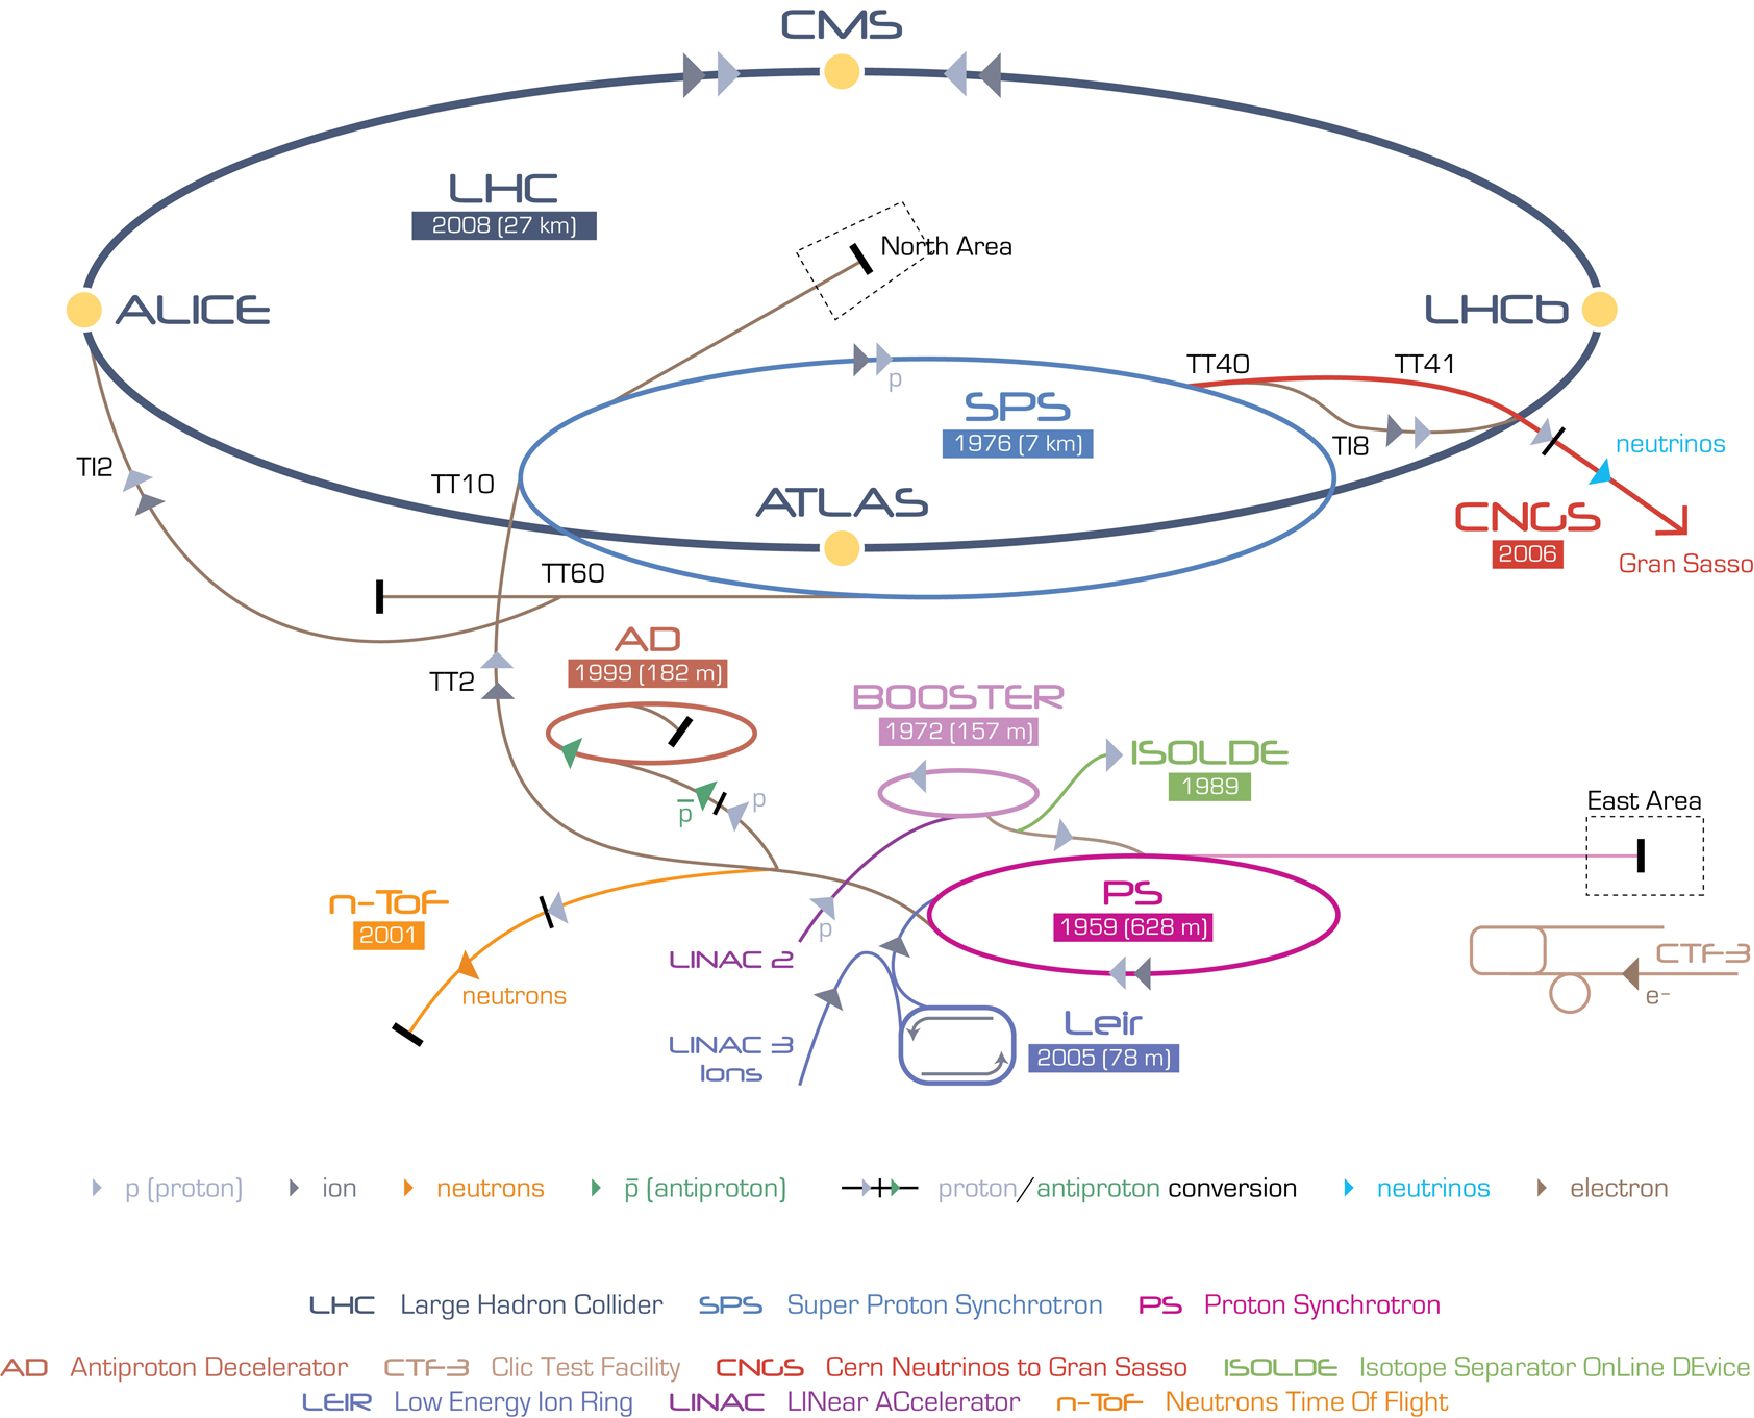
\includegraphics[width=\linewidth]{Chapters/Introduction/Figs/Cern-Accelerator-Complex.pdf}
\caption{Schematic representation of the CERN accelerator complex. \href{https://www.researchgate.net/publication/325961875_DEVELOPMENT_AND_EVALUATION_OF_NOVEL_LARGE_AREA_RADIATION_HARD_SILICON_MICROSTRIP_SENSORS_FOR_THE_ATLAS_ITk_EXPERIMENT_AT_THE_HL-LHC}{[source]}}
\label{fig:accelerators}
\end{center}
\end{figure}

The LHC allows one to perform proton-proton, proton-Pb and Pb-Pb collisions (and lately also Xe-Xe).
For what concerns the pre-acceleration of protons the CERN LInear ACcelerators (LINAC), the Proton Synchrotron Booster (PSB), the Proton Synchrotron (PS) and the Super Proton Synchrotron are used upstream the LHC.
The heavy nuclei are instead firstly produced, ionized and accelerated in the Low Energy Ion Ring (LEIR) and then injected directly in the PS-SPS chain.
Thanks to the superconducting magnets (dipoles, quadrupoles and higher order ones) protons and nuclei can be accelerated by design up to $7$ TeV and $2.75$ TeV respectively.
Such energy has not been achieved yet, due to insufficient magnets performance, instead the maximum reached energies were $6.5$ and $2.5$ TeV.
Along the LHC ring four main experiments are placed: ALICE (A Large Ion Collider Experiment),  ATLAS (A Toroidal LHC ApparatuS), CMS (Compact Muon Solenoid) and LHCb (Large Hadron Collider beauty).

%********************************** %Third Section  *************************************
\section{ALICE experimental setup} %Section - 1.3
\label{ALICE_apparatus}
The main purpose of the ALICE experiment is the study of the physics of strongly interacting matter in ultra-relativistic heavy-ion collisions. It is also designed for proton-proton and proton-nucleus collisions which represent an important part of its physics program. The experiment itself can be divided into three main sectors:
\begin{itemize}
    \item ancillar detectors are used for triggering, event characterization and beam luminosity measurements;
    \item central barrel detectors are embedded into a solenoid with a magnetic field of $B = 0.5$ T and are used for tracking and identification of charged particles and photons;
    \item muon spectrometer covers the forward region with respect to the interaction point and its detectors are designed for muon tracking and trigger.
\end{itemize}

\begin{figure}[!h]
\begin{center}
\includegraphics[width=\linewidth]{Chapters/Introduction/Figs/ALICE-Setup.pdf}
\caption{Schematic of ALICE detectors setup, with a maximised view of the innermost detectors. \href{http://aliceinfo.cern.ch/Public/en/Chapter2/Chap2Experiment-en.html}{[source]}}
\label{fig:ALICEsetup}
\end{center}
\end{figure}

The detector is completed by an array of scintillators to trigger on cosmic rays.
A more detailed discussion of the ALICE detectors is reported in the following sections.

\subsection{V0 and Zero Degree Calorimeters (ZDC)}
The two most relevant ancillar detectors for the work described in this thesis are introduced below.

\subsubsection{ZDC}
The main task performed by these calorimeters is the estimation of the collision centrality via the energy deposited by the spectator nucleons. 
There are two ZDCs, each composed of a neutron detector (ZN) and a proton detector (ZP).
They are located $\pm113$ m away from the IP; at such distance, protons and neutrons are spatially separated by the LHC magnetic elements: for this reason, while the neutron calorimeter is placed at zero degrees with respect to the LHC beam axis, the proton calorimeter is displaced (see Fig. \ref{fig:ZDC}).

\begin{figure}[!h]
\begin{center}
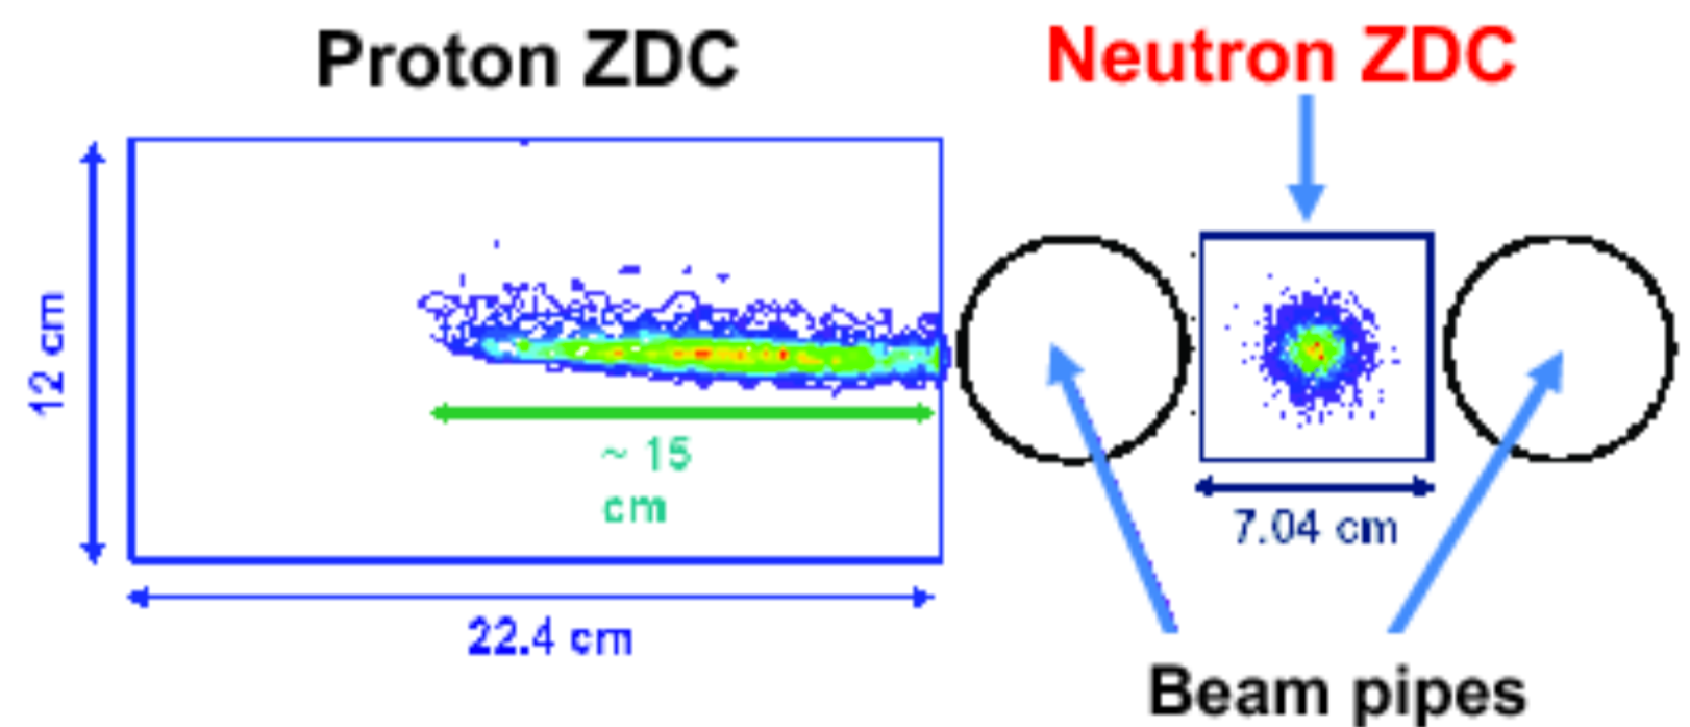
\includegraphics[width=.5\linewidth]{Chapters/Introduction/Figs/ZDC.pdf}
\caption{Schematic representation of the ZDC along the z-axis. The trasverse positions of the beam pipes, ZN and ZP are shown. From \cite{Oyama:2013xra}}
\label{fig:ZDC}
\end{center}
\end{figure}

\begin{figure}[!h]
\begin{center}
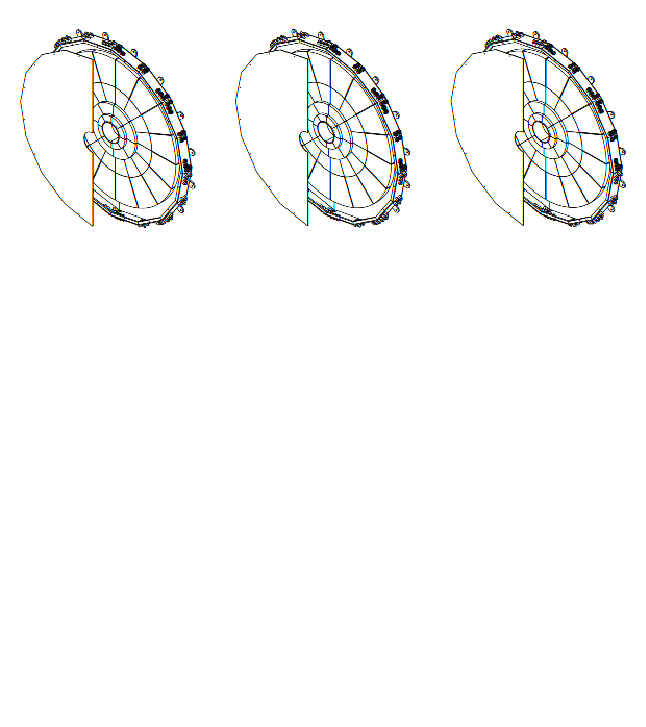
\includegraphics[width=.7\linewidth]{Chapters/Introduction/Figs/V0.pdf}
\caption{Schematic representation of one of the two V0 arrays (V0$_A$).}
\label{fig:V0}
\end{center}
\end{figure}

\subsubsection{V0}
The V0 detector (Fig. \ref{fig:V0}) is composed of two scintillator hodoscopes located at $90$ cm (V0$_C$, muon spectrometer side) and $-340$ cm (V0$_A$, PMD side) from the interaction point. 
Its main tasks are the delivery of minimum bias and centrality triggers, the offline estimation of centrality, the rejection of beam-gas interactions and the measurement of luminosity.

\subsection{Central barrel detectors}
The mid-rapidity section of the ALICE experimental apparatus is named central barrel.
It includes many detectors, each of them with different purposes.
The structure surrounds the interaction point, covering the pseudorapidity range up to $|\eta| < 1.4$, and it is inside the $0.5$ T magnetic field generated by a warm solenoidal magnet originally employed by the L3 collaboration.

\subsubsection{Inner Tracking System (ITS)}
The ITS is the closest detector to the beam pipe of the ALICE apparatus.
Its purposes are the identification of primary collision vertexes, the reconstruction of secondary vertexes from heavy particles decays and the tracking and identification of low momentum particles.
The spatial resolution of the ITS is better than $100\ \mathrm{\mu m}$.
It is completely made of silicon detectors, implemented using three technologies.
Six layers compose the ITS and are shown in Fig. \ref{fig:ITS}:
\begin{itemize}
    \item Silicon Pixel Detector (SPD): two layers located at $3.9$ and $7.6$ cm from the interaction point, they are important for a high spatial resolution and for their very fast response;
    \item Silicon Drift Detector (SDD) : two layers located at $15$ and $23.9$ cm from the interaction point, they provide a bi-dimensional spatial information;
    \item Silicon Strip Detector (SSD) : two layers located at $38$ and $43$ cm from the interaction point, they provide a complementary information on track positions.
\end{itemize}


\begin{figure}[!h]
\begin{center}
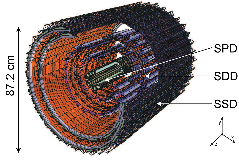
\includegraphics[width=0.7\linewidth]{Chapters/Introduction/Figs/its.pdf}
\caption{Schematic of the ALICE ITS.  From \cite{Aamodt:2010aa}}
\label{fig:ITS}
\end{center}
\end{figure}

\subsubsection{Time Projection Chamber (TPC)}
The Time Projection Chamber is the main tracking detector of the central barrel.
It is a $88\ \rm m^3$ cylindrical detector filled with a gas mixture of $Ar-CO_2\ (90-10 \% )$ for most of the operation time.
Its volume is limited by two end-plates acting as segmented read-out electrodes. 
In addition an electrode is placed in the middle of the TPC, dividing it into two halves, as shown in figure \ref{fig:TPC}.
The ionizing particles crossing the detector ionize the gaseous mixture.
The freed electrons drift towards the read-out electrodes.
As a result the side projection of the track is obtained directly from the electrodes, while the third coordinate of the points is obtained through the time of arrival of each segment.

\begin{figure}[!h]
\begin{center}
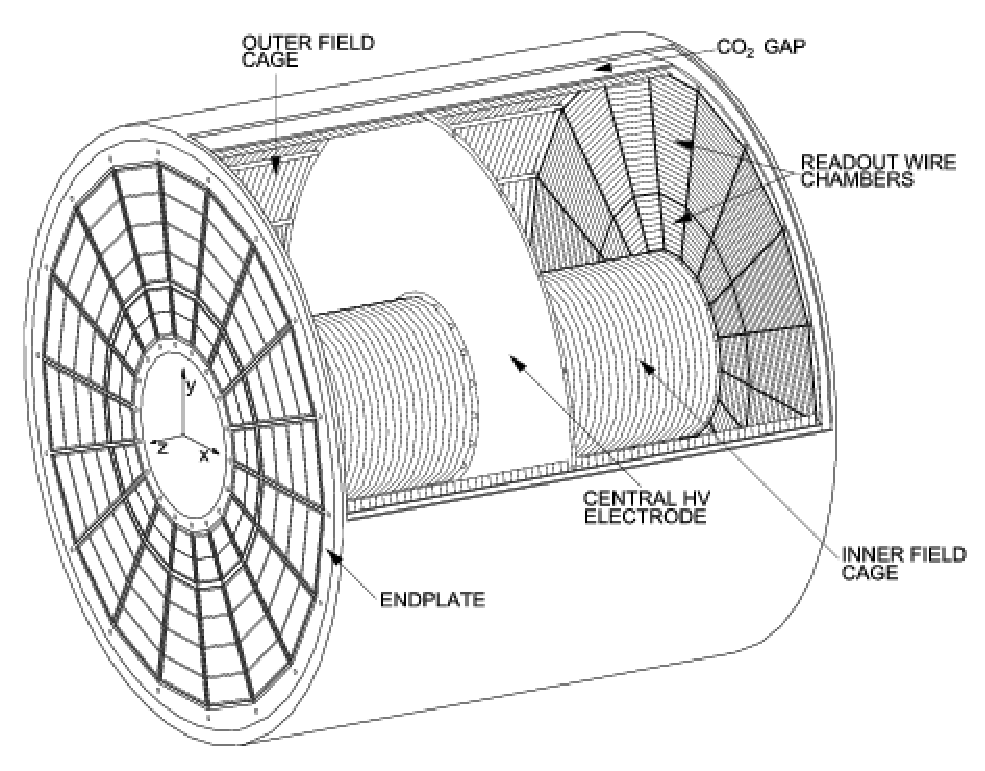
\includegraphics[width=0.7\linewidth]{Chapters/Introduction/Figs/tpc.pdf}
\caption{Representation of the TPC with some details of the layout. From \cite{Alme:2010}}
\label{fig:TPC}
\end{center}
\end{figure}

\subsubsection{Transition Radiation Detector (TRD)}
The purpose of the Transition Radiation Detector is the electron identification.
It consists of six layers of multi-wire proportional chambers, filled with a mixture of $Xe$ and $CO_2$, equipped with a radiator made of optical fibers embedded in plastic foam directly glued on the electrode.
The modular structure is detailed in figure \ref{fig:TRD}.
It is designed to provide charged-particle tracking, electron identification via transition radiation and pion rejection. 
% The combination of ITS, TPC and TRD information provides a momentum resolution in the central barrel good enough to measure high pt tracks down to $100\ GeV/c$ and a mass resolution about $100\ MeV/c$.

\begin{figure}[!h]
\begin{center}
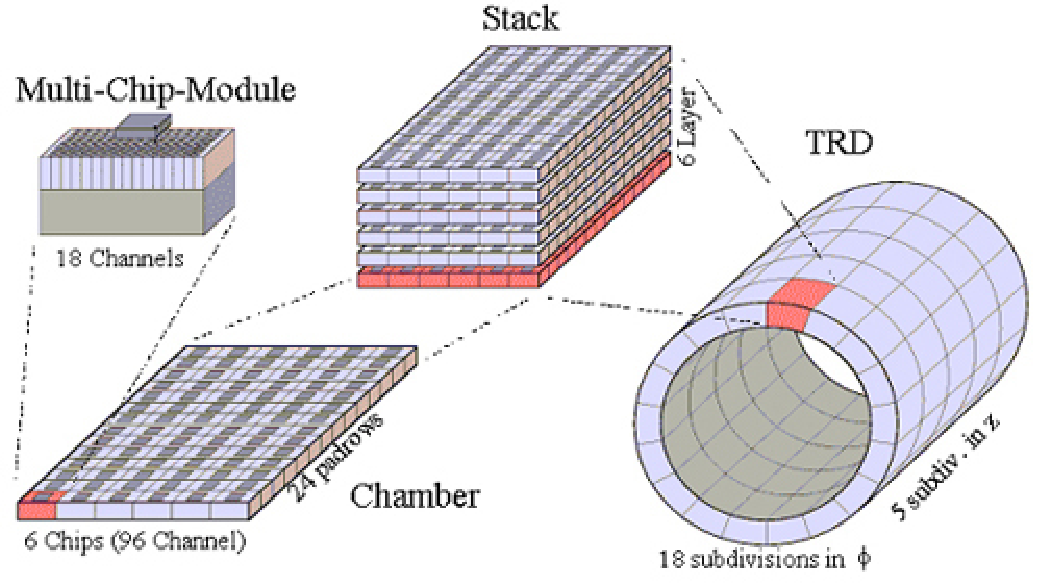
\includegraphics[width=0.7\linewidth]{Chapters/Introduction/Figs/trd.pdf}
\caption{Schematic of the ALICE TRD with an highlight on the modular struture of the detector. \href{http://www.lhc-facts.ch/index.php?page=alice}{[source]}}
\label{fig:TRD}
\end{center}
\end{figure}

\subsubsection{Time Of Flight (TOF)}
The Time Of Flight detector is designed to identify charged particles with a momentum from $1$ to few GeV/c, extending the TPC particle identification capabilities. 
It is composed by multi-gap resistive plate chambers arranged into $18$ sectors in a cylindrical shell placed $3.7$ m far from the beam pipe (Fig. \ref{fig:TOF}). 
The TOF provides the arrival time of a particle in the detector volume with a resolution of $80$ ps, completing the information gathered by TPC and TRD, in terms of identification of the detected particles, in particular separating $\pi/K$ up to $2.2$ GeV/c and $K/p$ up to $4$ GeV/c.

\begin{figure}[!h]
\begin{center}
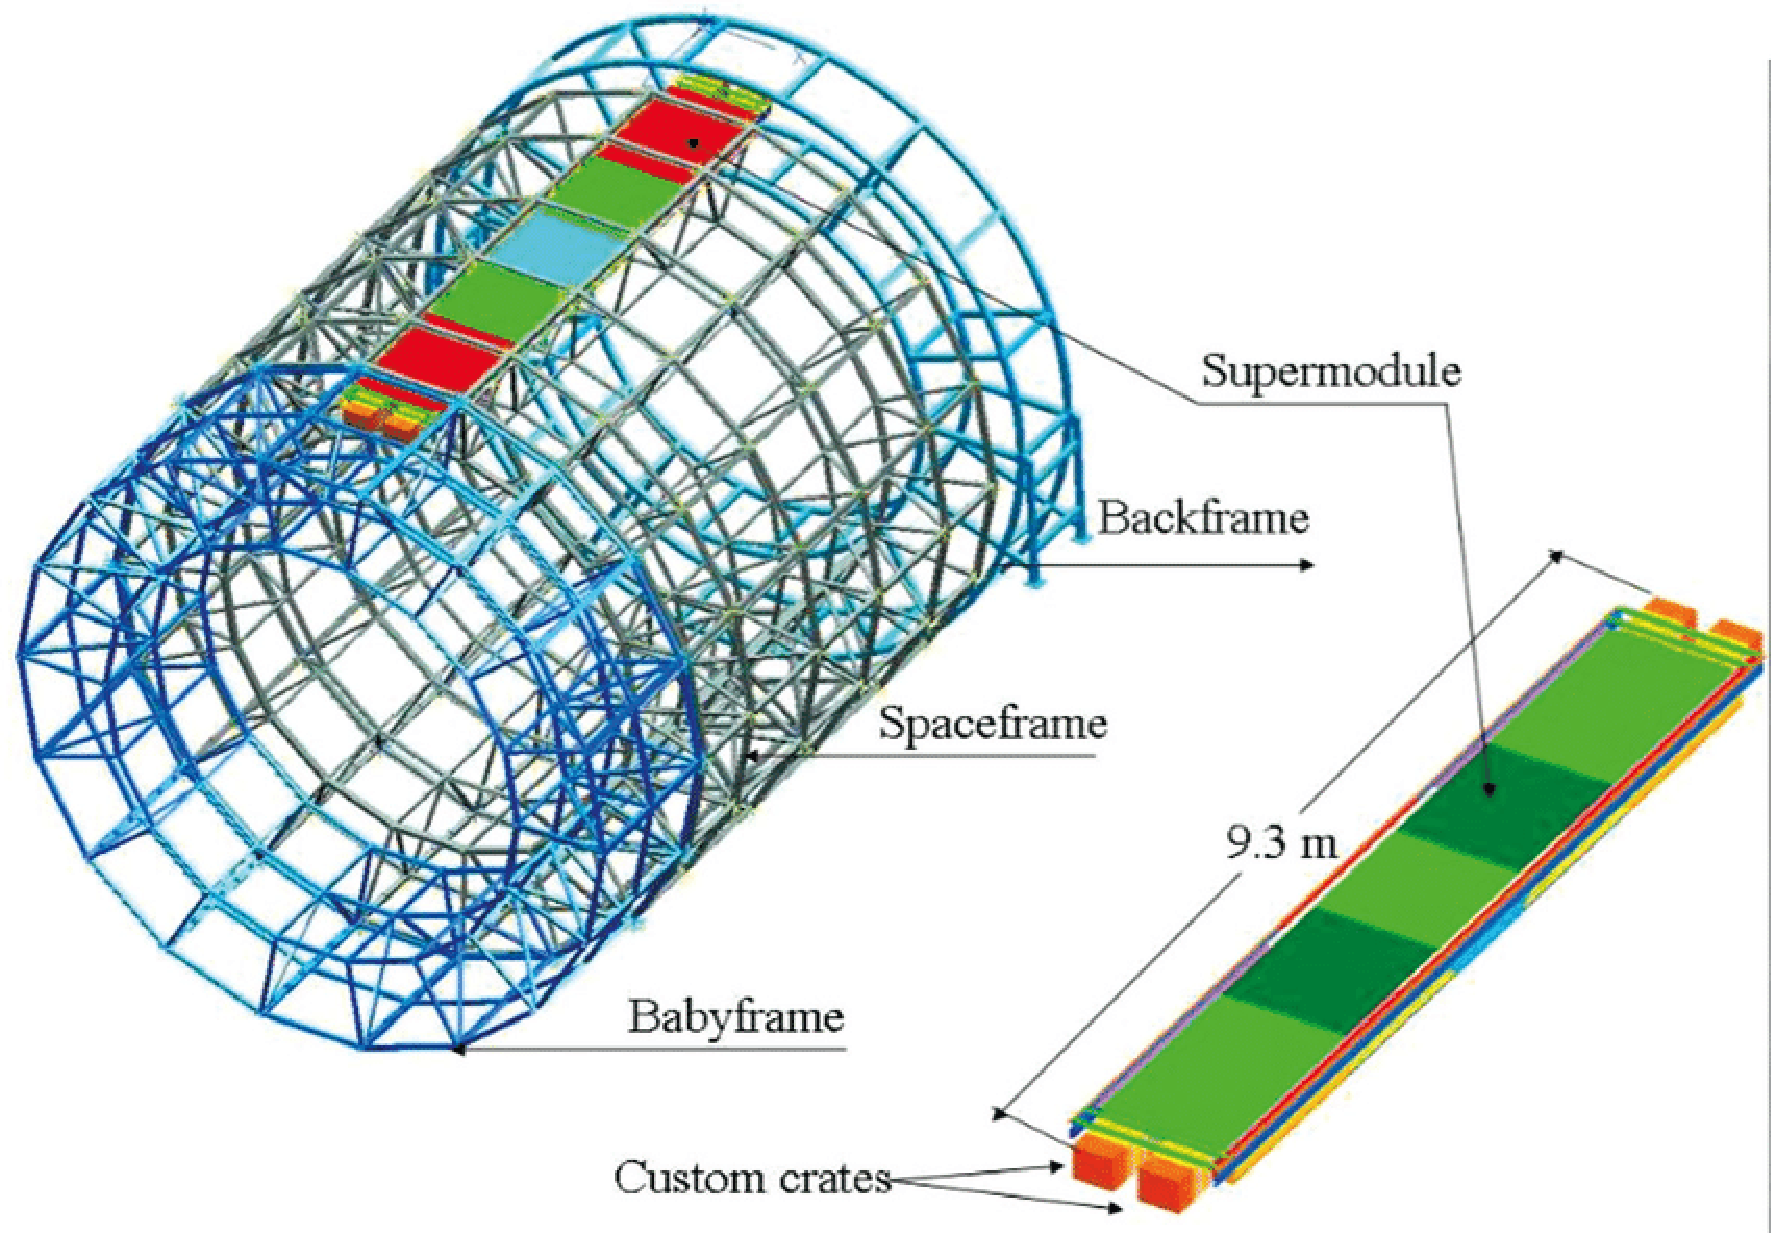
\includegraphics[width=0.7\linewidth]{Chapters/Introduction/Figs/tof.pdf}
\caption{Schematic of the ALICE TOF. A detector module is represented along with the support structure. From \cite{Adam:2017}}
\label{fig:TOF}
\end{center}
\end{figure}

\subsubsection{High Momentum Particle Identification Detector (HMPID)}
The main purpose of HMPID is to enhance the particle identification capability beyond the range allowed by ITS, TPC and TOF. 
It is based on proximity focusing Ring Imaging Cherenkov (RICH) counters and consists of seven modules mounted in an independent support cradle (Fig. \ref{fig:HMPID}). 
When a fast charged particle traverses the $15$ mm layer of liquid $C_6F_{14}$, Cherenkov photons are emitted and detected by the photon counter, which is a thin layer of $CsI$ deposited onto the pad cathode of multi-wire proportional chambers.

\begin{figure}[!h]
\begin{center}
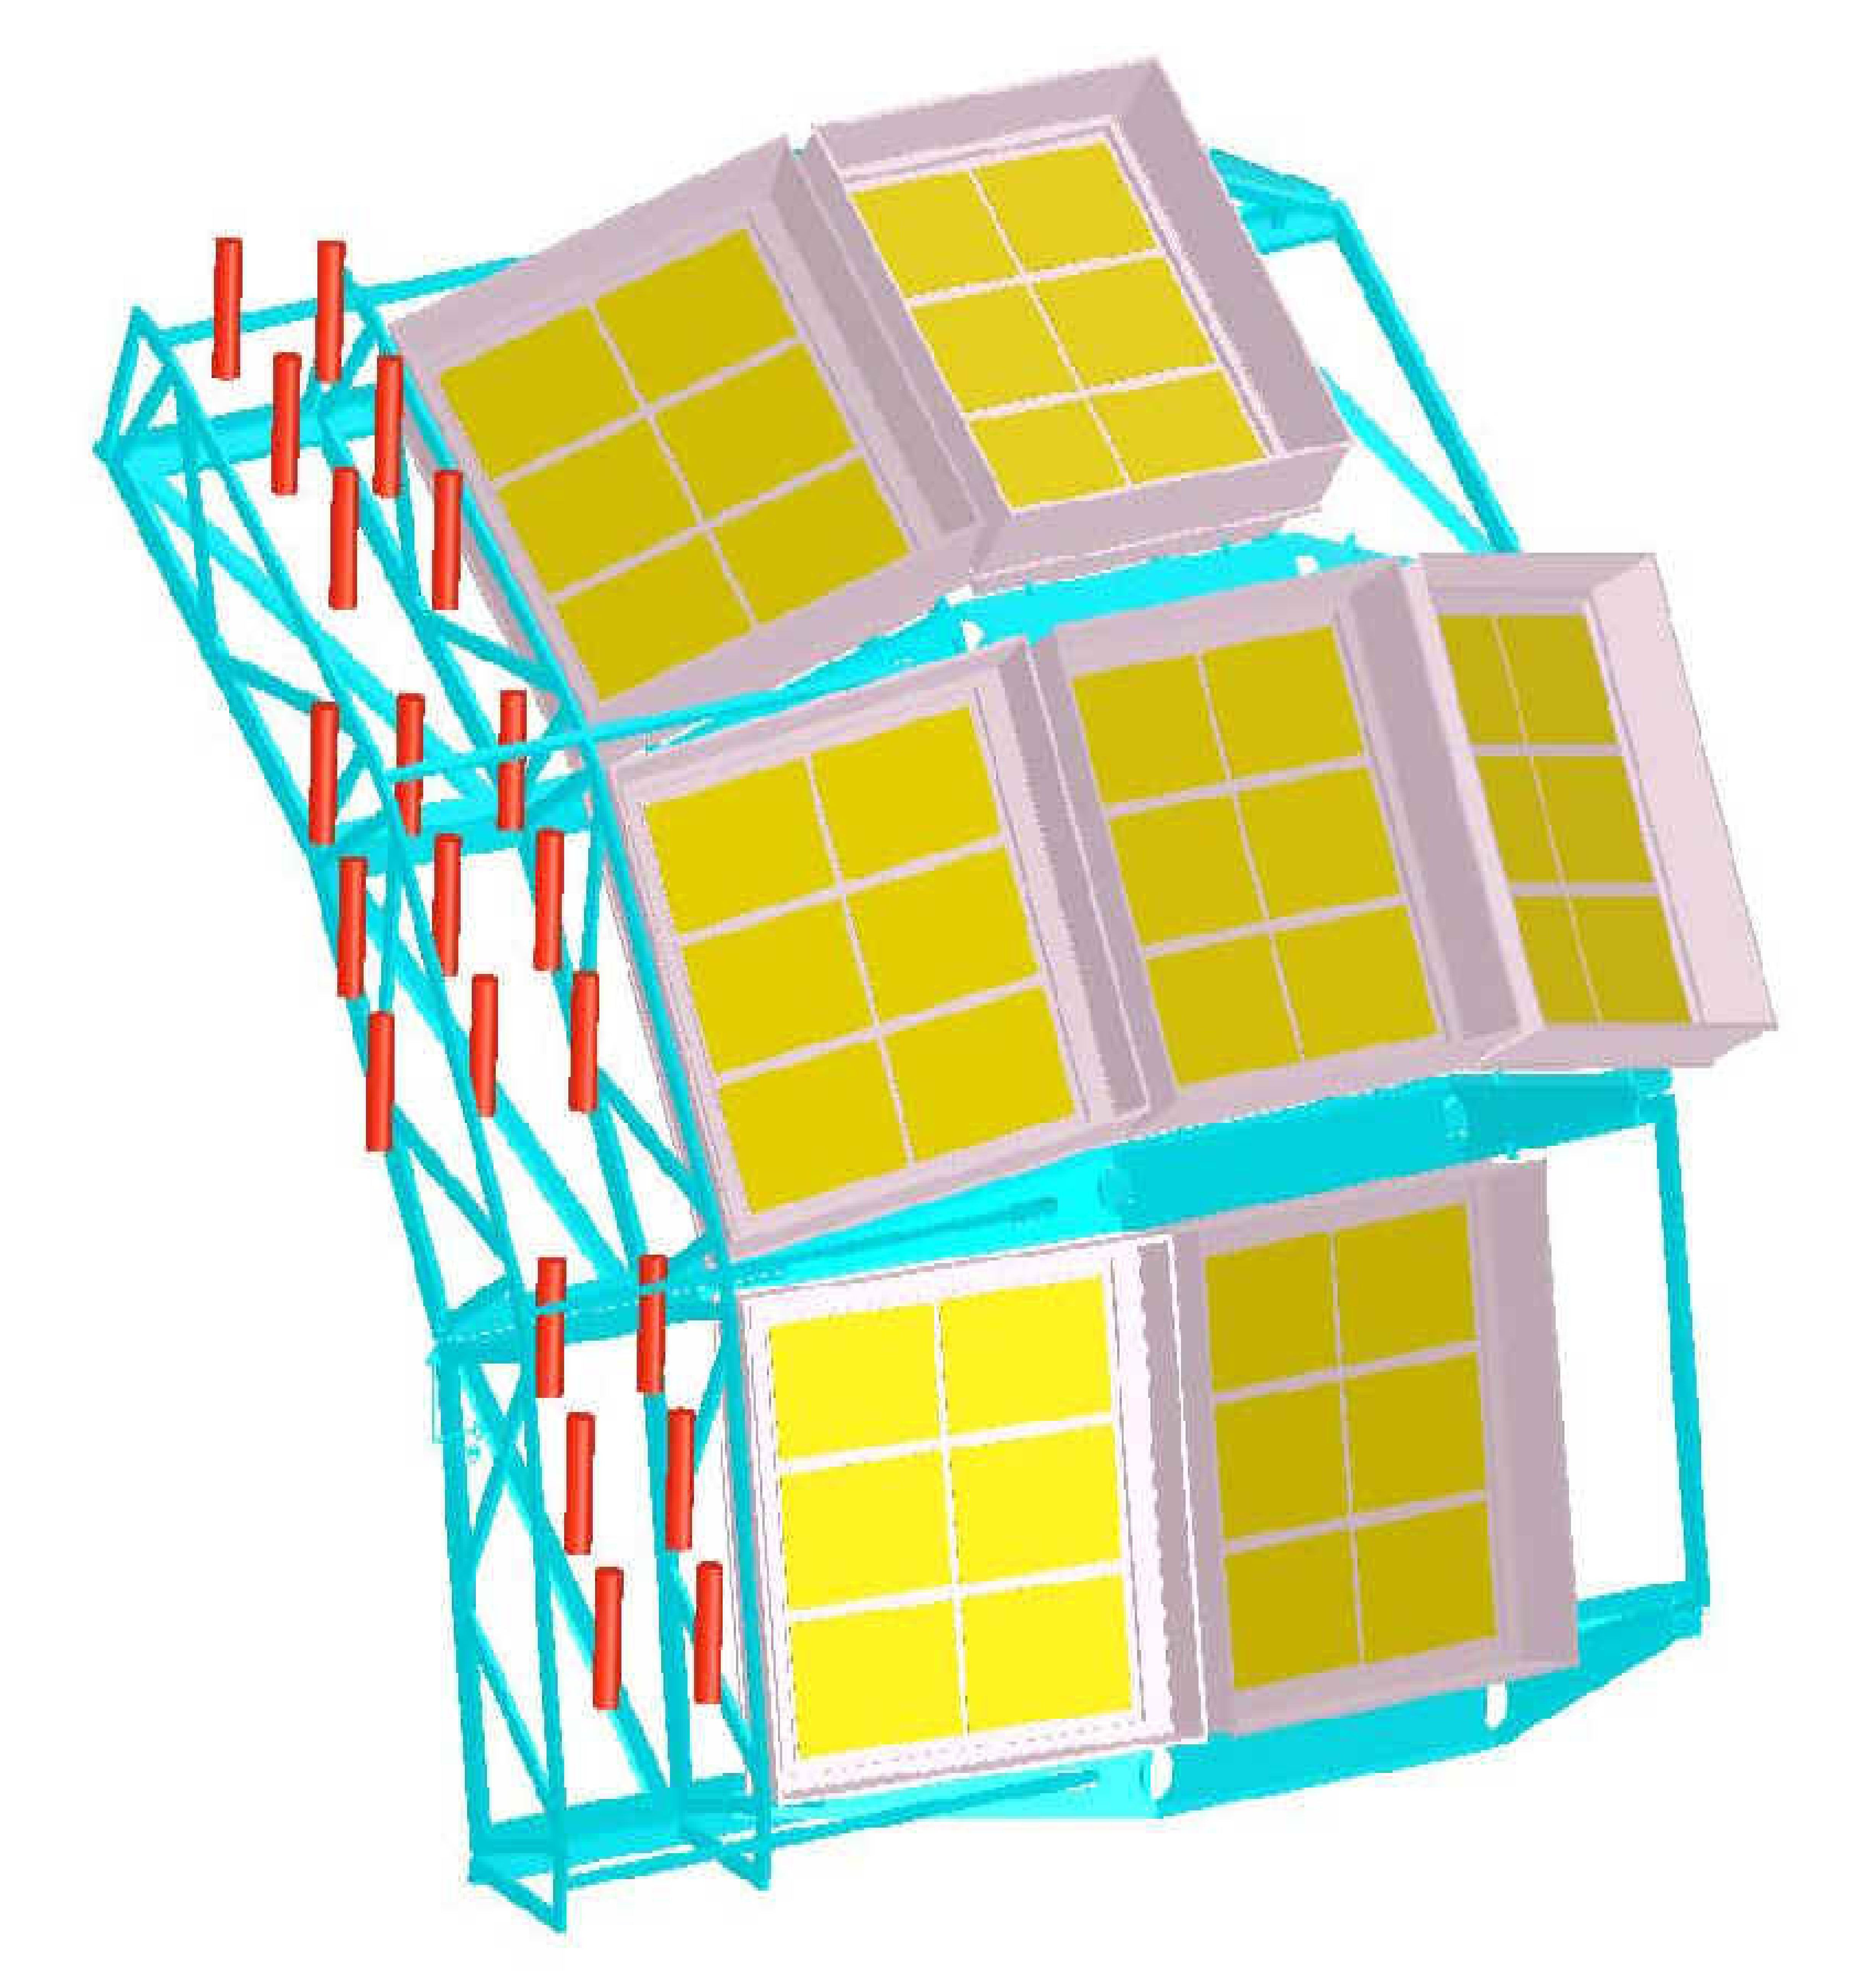
\includegraphics[width=0.4\linewidth]{Chapters/Introduction/Figs/hmpid.pdf}
\caption{The HMPID layout. \href{http://alice.web.cern.ch/detectors/more-details-alice-hmpid}{[source]}}
\label{fig:HMPID}
\end{center}
\end{figure}

\subsubsection{PHOton Spectrometer (PHOS)}
The Photon Spectrometer is a high resolution electromagnetic spectrometer (Fig. \ref{fig:PHOS}) which consists of a highly segmented electromagnetic calorimeter of lead-tungstate crystals.
It is located on the bottom of the ALICE experimental apparatus, covering the pseudorapidity range $|\eta| < 0.12$ and an interval of $\frac{5}{9}\pi$ radiants in the azimuthal angle.
It is designed for measuring photons and neutral mesons ($\pi_0$ and $\eta$) through their decays into two photons up to momenta about $10$ GeV/c.

\begin{figure}[!h]
\begin{center}
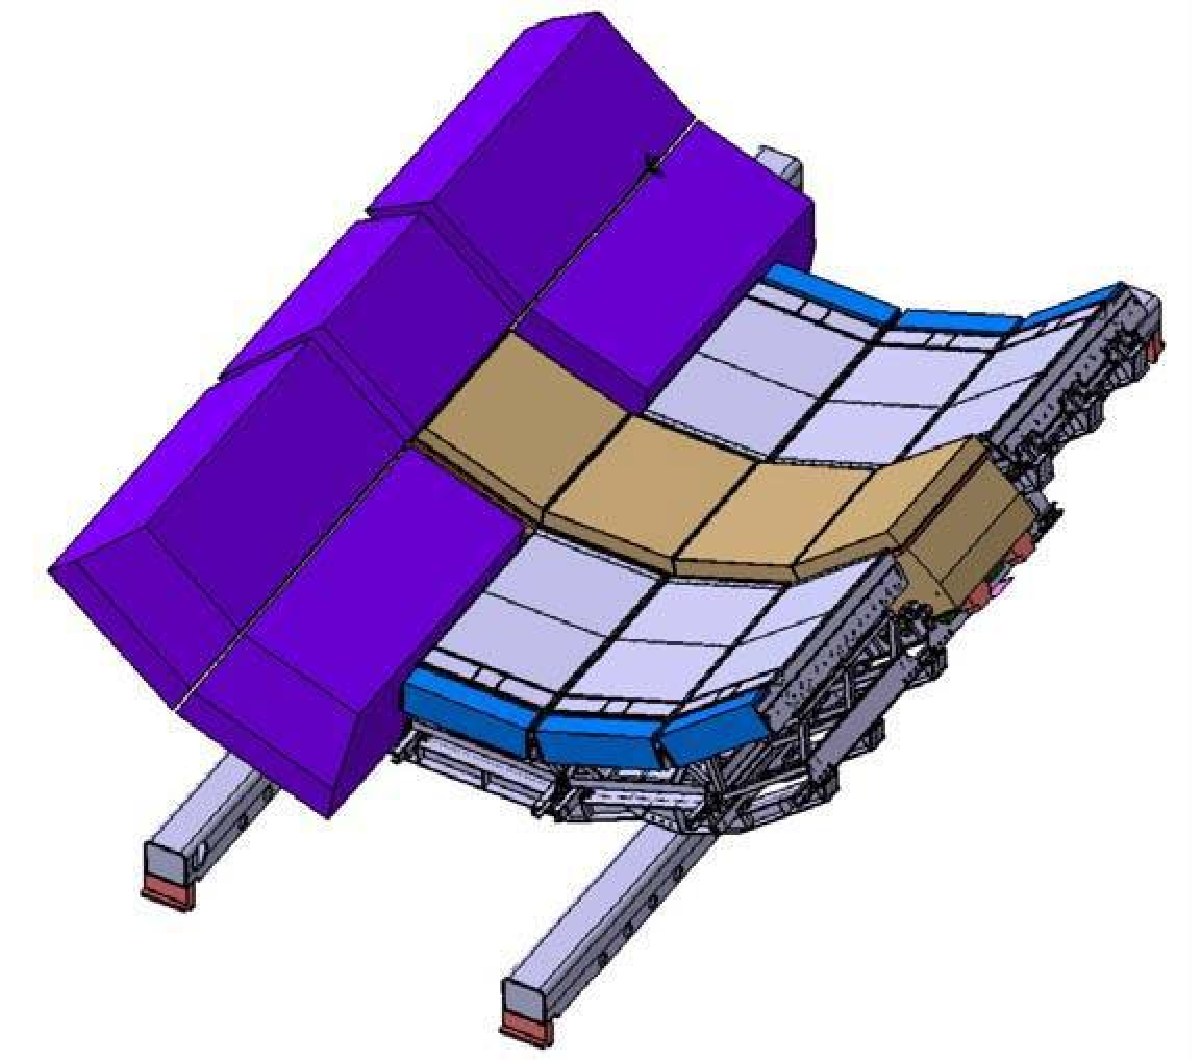
\includegraphics[width=0.5\linewidth]{Chapters/Introduction/Figs/phos.pdf}
\caption{The PHOS layout (brown) along with the DCal detector arrays (blue and light blue). \href{http://alice.web.cern.ch/detectors/more-details-alice-dcal}{[source]}}
\label{fig:PHOS}
\end{center}
\end{figure}

\subsubsection{ElectroMagnetic Calorimeter (EMCal) and Di-jet Calorimeter (DCal)}
Positioned on the top and bottom of the ALICE structure, close to the solenoid coils, EMCal is designed to study jet quenching and it is used for triggering on photons, electrons and jets.
It is composed of towers of lead scintillators with photomultiplier readout and it covers a pseudo-rapidity range of $|\eta| < 0.7$ (Fig. \ref{fig:EMCAL}).
The Di-jet calorimeter is an additional array of electromagnetic calorimeter which expands the acceptance of EMCal, allowing for back-to-back correlations (Fig. \ref{fig:PHOS}).

\begin{figure}[!h]
\begin{center}
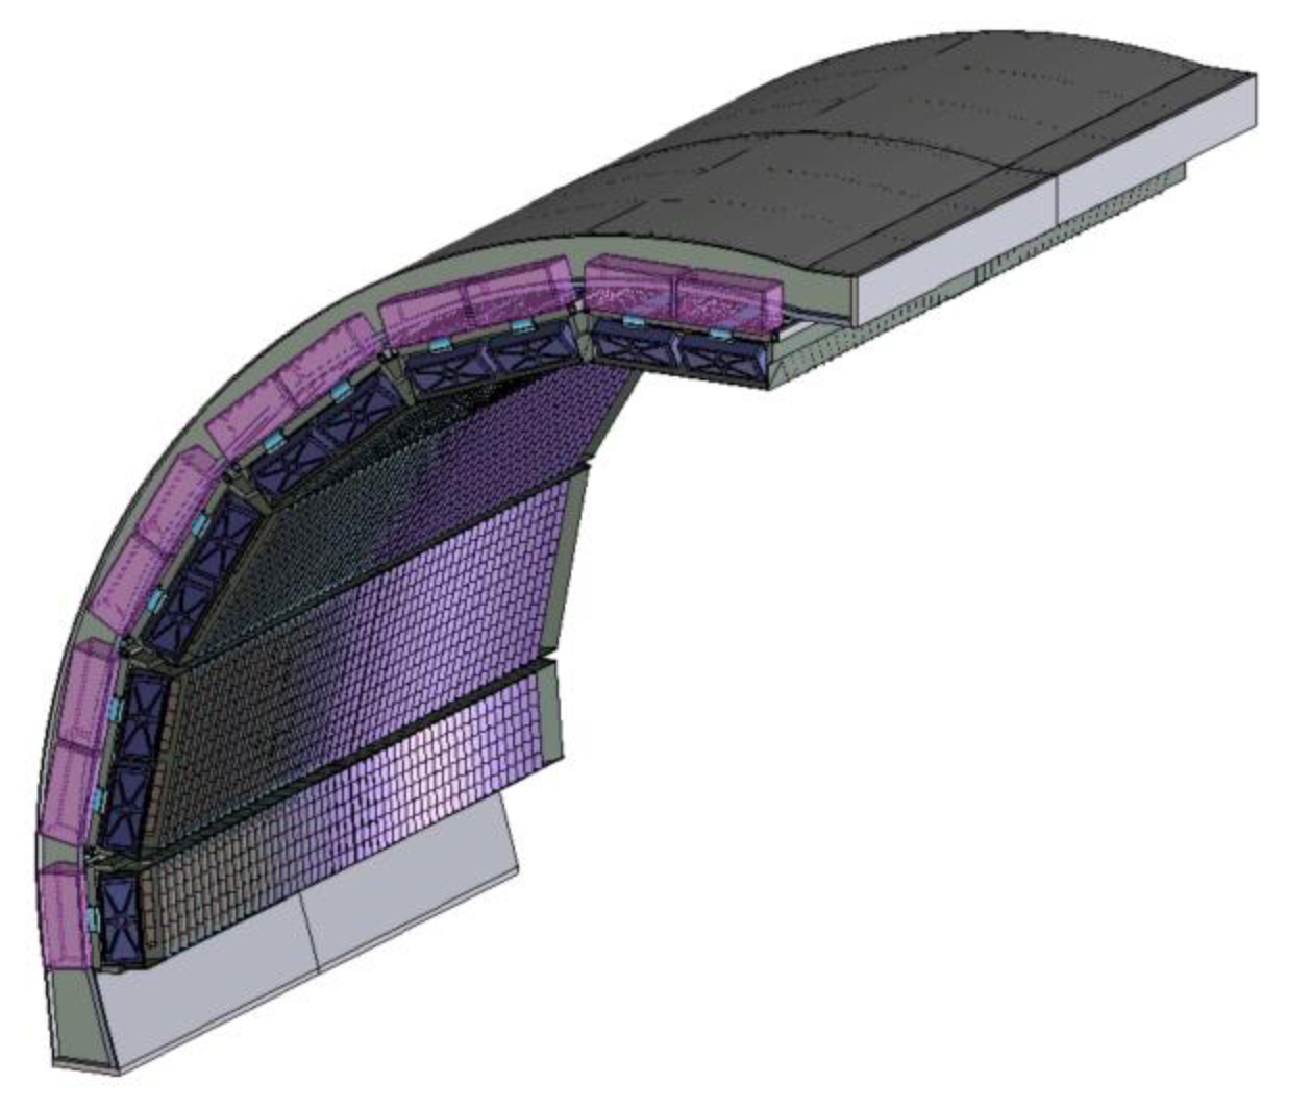
\includegraphics[width=0.5\linewidth]{Chapters/Introduction/Figs/emcal.pdf}
\caption{The EMCal layout. \href{https://trac.cc.jyu.fi/projects/alice/wiki/EMCAL}{[source]}}
\label{fig:EMCAL}
\end{center}
\end{figure}

\subsection{Muon spectrometer}
\label{ALICE_spectrometer}
The Muon Spectrometer is designed to measure muon production from the decays of quarkonia ($J/\psi$ , $\psi(2S)$ , $\Upsilon(1S)$, $\Upsilon(2S)$ and $\Upsilon(3S)$), low mass vector mesons ($\rho$, $\omega$ and $\phi$) and heavy flavor hadrons.
In addition it also allows for the measurement of $W^\pm$ and $Z^0$ bosons. 
The detector is covers the pseudorapidity region $-4.0 < \eta < -2.5$ and it has a total length of $\simeq 17$ m.
For the sake of readability, the rapidity acceptance of the spectrometer and the rapidity ranges quoted in this thesis will be reported as positive ranges instead (\textit{e.g.} $2.5 < y < 4.0$).
It is composed by a system of passive absorbers, a dipole magnet, a muon tracker, an iron wall and a muon trigger system. 
The main components of the Muon Spectrometer will be discussed with more details in the following and are highlighted in figure \ref{fig:spectro}.

\begin{figure}[!h]
\begin{center}
\includegraphics[width=\linewidth]{Chapters/Introduction/Figs/spectro.pdf}
\caption{Schematic representation of ALICE with highlighted muon spectrometer components. \href{http://irfu.cea.fr/en/Phocea/Vie_des_labos/Ast/ast_sstechnique.php?id_ast=2245}{[source]}}
\label{fig:spectro}
\end{center}
\end{figure}

\subsubsection{Absorbers system}
The Muon Spectrometer requires some shielding to reduce the otherwise large background produced especially in nucleus-nucleus collisions.
For this reason it is equipped with a system of absorbers:
\begin{itemize}
    \item front absorber: this absorber is located as close as $90$ cm from the interaction point. The purpose of the front absorber is to filter out hadrons and to reduce the background generated by pion and kaon decays. The front absorber materials were chosen to limit the multiple scattering of muons and leptons in general. The section of the front absorber placed closest to the interaction point is made of carbon to limit multiple scattering thanks to the low Z. The next sections of the absorber are composed of concrete to absorb secondary particles and low energy protons and neutrons. The whole absorber is coated of lead and boronated polyethilene to avoid decay products recoils in the TPC. A detailed view of the absorber can be found in figure \ref{fig:absorber};
    \item beam shield: the beam pipe is layered with this shielding made of tungsten, lead and stainless steel to shield the muon spectrometer from the particles produced in the interactions between low angle particles and gas residuals inside the beam pipe itself;
    \item iron wall: this $1.2$ m thick absorber is placed between two detector systems and acts as a filter capable of absorbing everything but muons;
    \item rear absorber: an additional passive element has been installed around the connection hole between the experiment cave with the LHC tunnel in order to further remove products of gas interaction.
\end{itemize}

\begin{figure}[!h]
\begin{center}
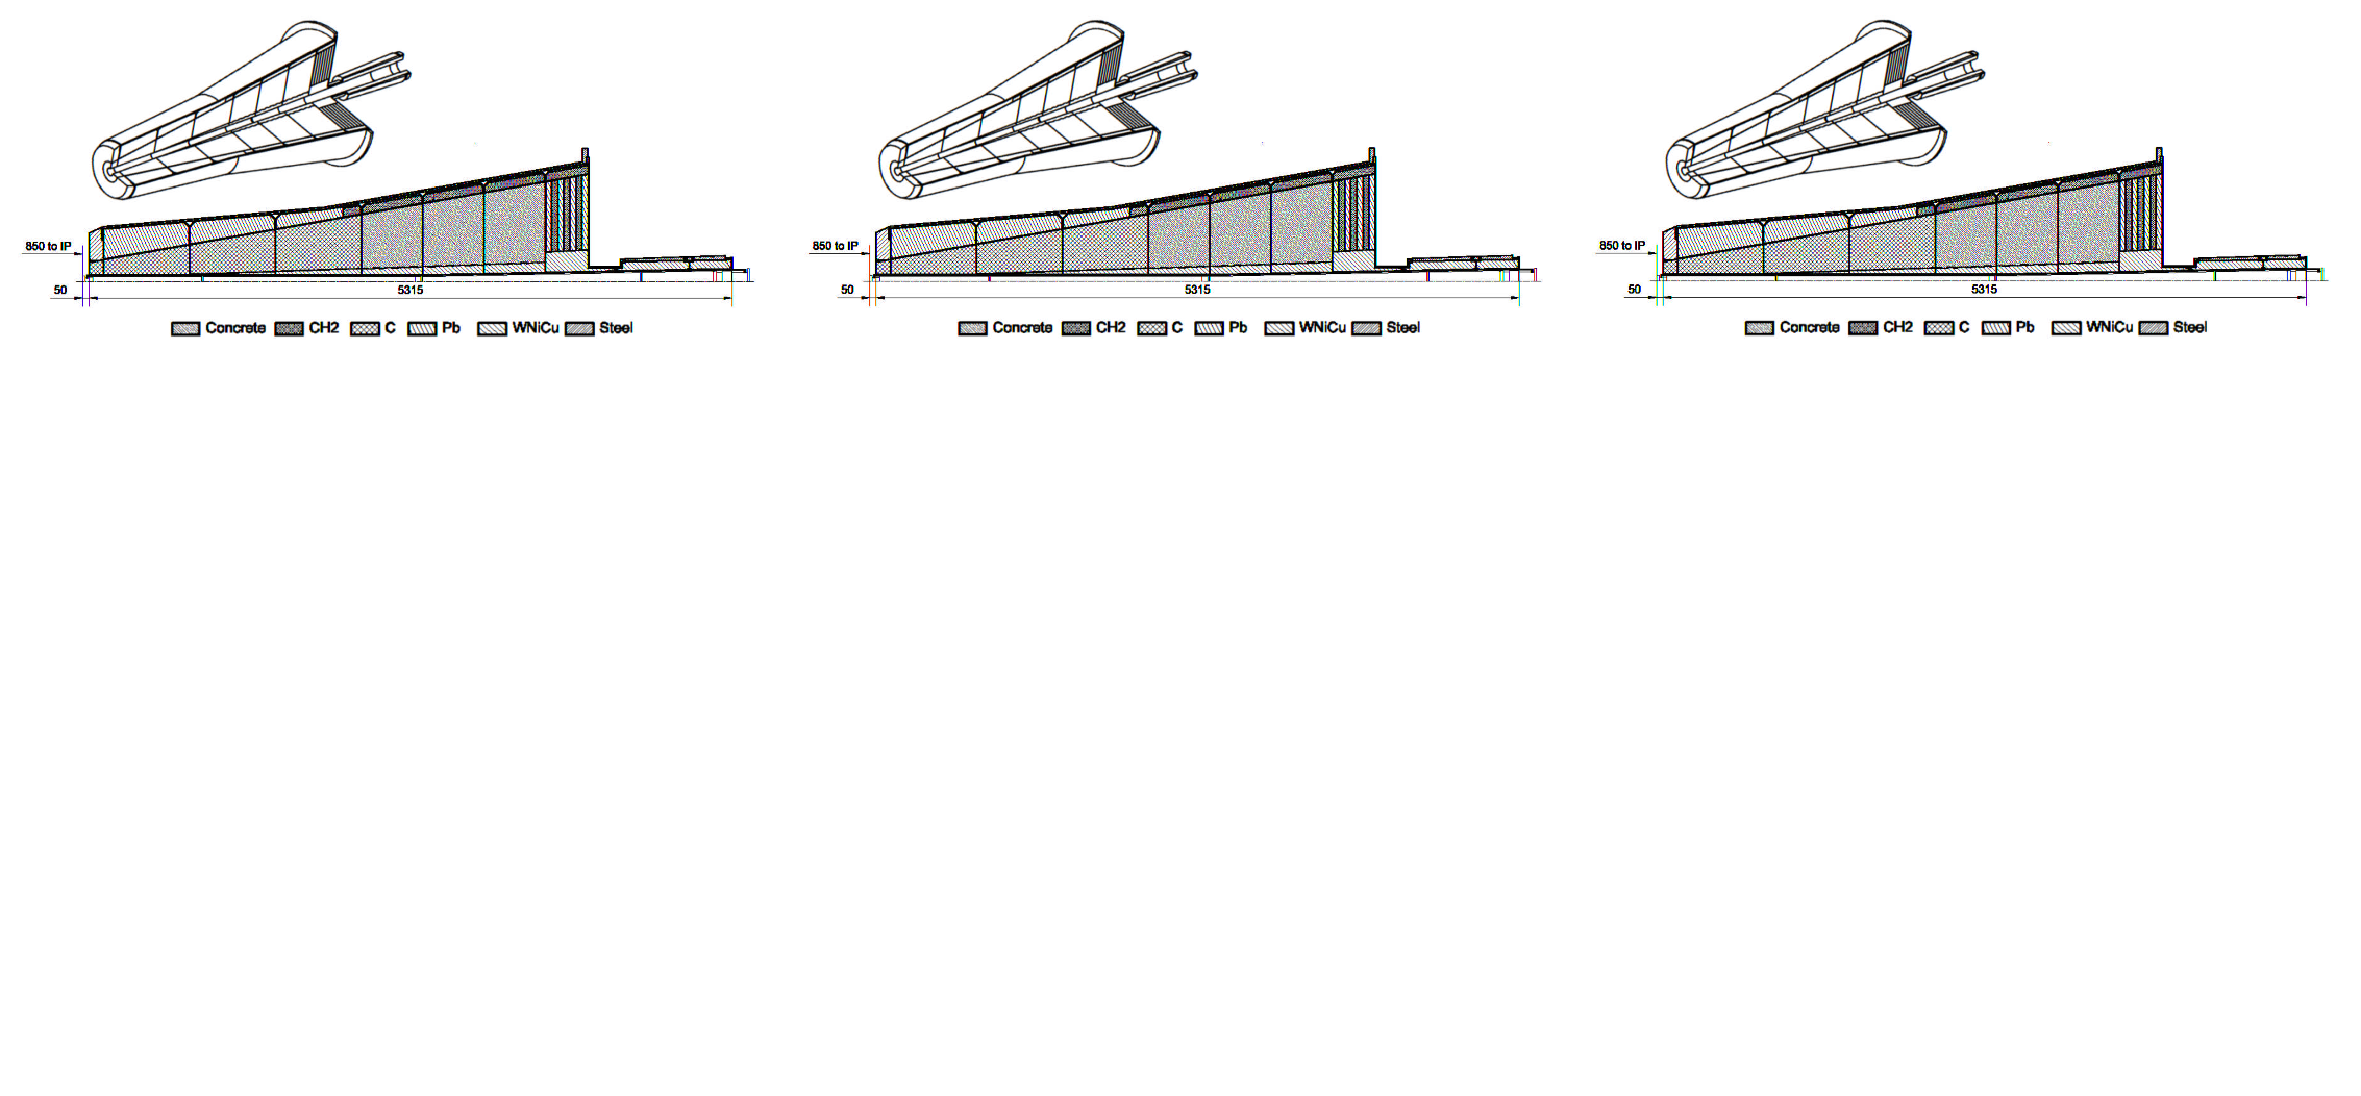
\includegraphics[width=0.7\linewidth]{Chapters/Introduction/Figs/absorber.pdf}
\caption{Detailed reprensentation of the front absorber composition.}
\label{fig:absorber}
\end{center}
\end{figure}

\subsubsection{Dipole magnet}
Located at $7$ m from the interaction point, the dipole magnet is used to bend the particle in such a way that the momentum and electric charge can be determined.
A schematic representation is reported in Fig. \ref{fig:dipole}.
The value of the magnetic field provided (the magnetic flux density is $0.7$ T and the integrated value is $3\ \mathrm{T\cdot~m}$) is defined by requirements of quarkonium mass resolution.
The magnetic field is perpendicular to the beam pipe.
% The definition of bending and non-bending planes follows the magnetic field direction.
The ALICE reference frame is a Cartesian tridimensional space in which the $z$ axis is placed along the beam direction, the $x$ axis is parallel to the ground and pointing to the center of the LHC and the $y$ axis vertical towards the top.
% The plane $zy$ is defined as the bending plane, since the dipole action deviates muons in this direction, and the plane $xz$ as the non-bending plane.
In this reference frame the magnetic field is directed along the $x$ axis. The charged particle are therefore deviated along $y$ (bending direction) while the $x$ direction is therefore referred to as non-bending.

\begin{figure}[!h]
\begin{center}
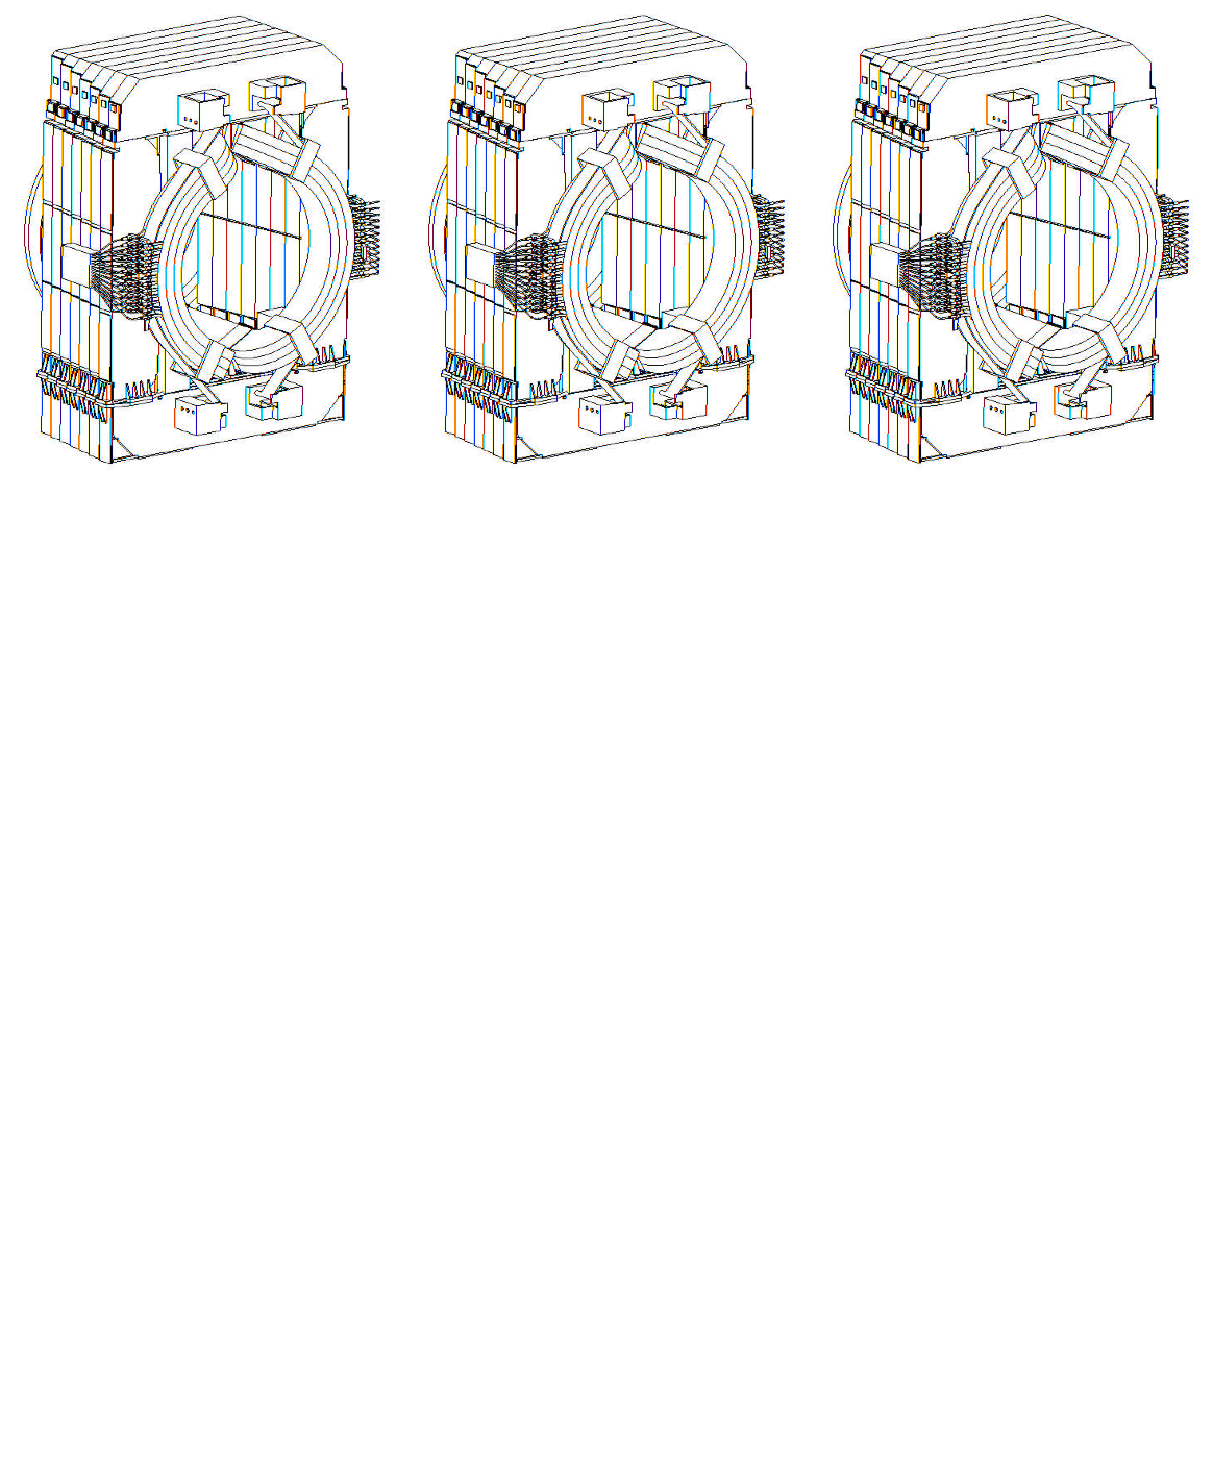
\includegraphics[width=0.6\linewidth]{Chapters/Introduction/Figs/dipole.pdf}
\caption{ALICE dipole magnet schematics.}
\label{fig:dipole}
\end{center}
\end{figure}

\subsubsection{Muon Tracker or Muon Chambers (MCH)}
The tracking system is made of $10$ detection planes made of multi wire proportional chambers arranged in $5$ stations of $2$ planes each (Fig. \ref{fig:mch_mtr}, round shaped layers).
% The anode is implemented as wires placed between the readout sides, while the readout electrodes are placed on the sides.
The produced electrons generate an avalanche drifting towards the nearest anode wire, and the resulting ion cloud induces a charge distribution on the cathode planes, allowing to determine the position of the impacting particle.
The size of the chambers depends on the spectrometer’s angular coverage, considering the deviation of muons by the magnetic field.
The pad size of all the chambers is smaller close to the beam pipe, in order to take into account the higher density of particles produced in that region.
The spatial resolution is better than $100\ \mathrm{\mu m}$ and all the chambers are made of composite material ($< 3\%$ $X_0$ per chamber) to minimize the scattering of the muons in order to obtain the required resolution. 
To limit the occupancy to a maximum of $5\%$ the full set of chambers has more than $1$ million channels.

\begin{figure}[!h]
\begin{center}
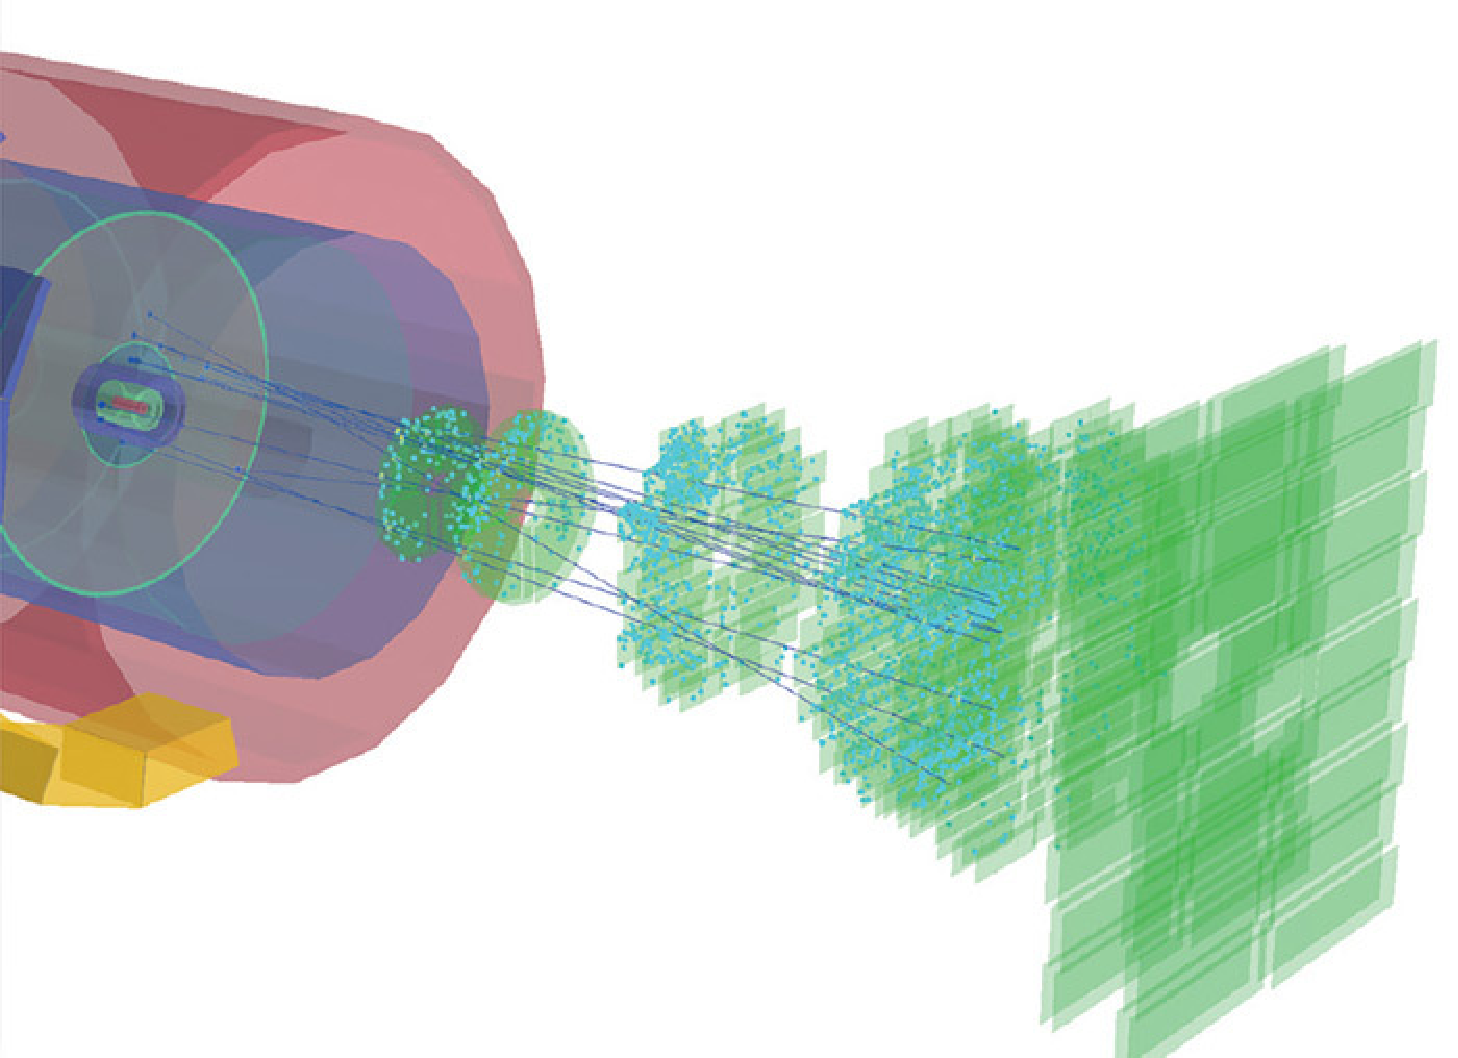
\includegraphics[width=\linewidth]{Chapters/Introduction/Figs/muon_mtr_mch.pdf}
\caption{Digital representation of the layout of the muon chambers and muon trigger system, shown in green.}
\label{fig:mch_mtr}
\end{center}
\end{figure}

\subsubsection{Muon Trigger (MTR)}
The muon trigger system is designed to tag high $p_T$ muons produced in heavy quarkonium and open heavy flavour meson decays (Fig. \ref{fig:mch_mtr}, square shaped layers).
Thank to a configurable $p_T$ threshold, the system is able to provide trigger signals to select interesting events and to discard events with only low $p_T$ muons, which mainly come from pions and kaons decays.
The muon trigger system is composed of 72 Resistive Plate Chambers with $x-y$ read out, organized in $4$ planes paired in two stations to provide redundancy.
Each RPC consists of two planes, made of bakelite and separated by $2$ mm of gas.
A charged particle passing through the gas ionizes it, causing the formation of an avalanche of secondary electrons, which are picked up by the copper strips placed outside the chambers.

\begin{figure}[!h]
\begin{center}
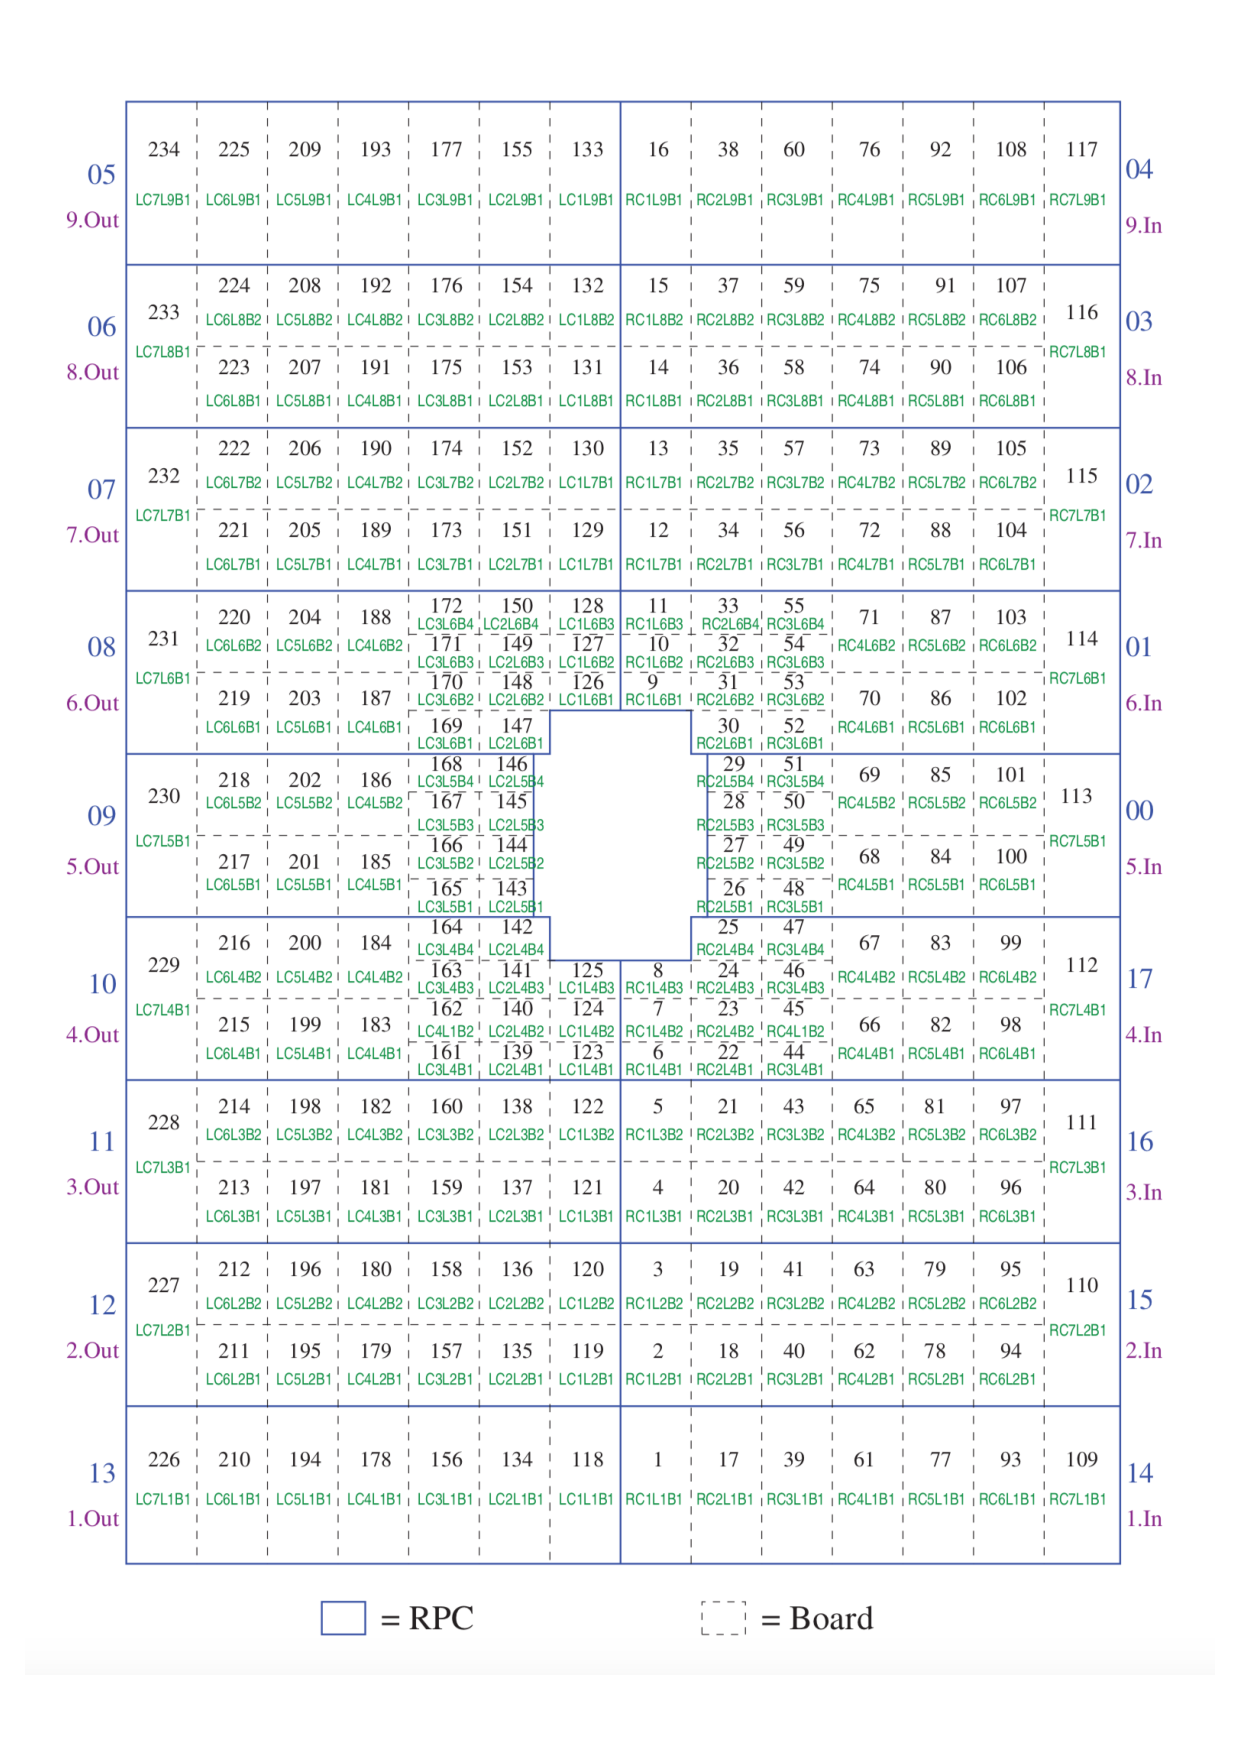
\includegraphics[width=0.65\linewidth]{Chapters/Introduction/Figs/LB.pdf}
\caption{Local Board segmentation of the ALICE Muon Trigger.}
\label{fig:LB}
\end{center}
\end{figure}

The read-out of the Muon Trigger System is performed through front-end electronics (FEE) boards connected to the strips.
Information collected by the FEE is aggregated at the level of the Local Boards (LB).
The ALICE MTR is equipped with a total of 234 local boards (Fig. \ref{fig:LB}).
The LBs collect the strip pattern of FEE boards aligned projectively on the four planes of the MTR.
In addition to the patterns of the directly aligned FEE boards, the output of the boards surrounding the corresponding one on the third and fourth planes are retrieved and combined at the LB level.
This procedure is necessary for the generation of the online trigger signal, obtained looking at the hits in the first and second planes and checking if any corresponding hit is present in the patterns of the third and fourth ones.
A hit on at least $3/4$ planes both in bending and non-bending directions is required to produce a trigger signal.

In order to be triggered a particle still has to pass the $p_{\mathrm{T}}$ cut.
Such selection is performed considering the deviation of a track with respect to the track with infinite momentum.
This deviation depends indeed on the $p_{\mathrm{T}}$ of the particle, being larger at low transverse momenta.
The actual estimation of the $p_{\mathrm{T}}$ is performed through the Look-Up Tables (LUT) which are filled according to Monte Carlo simulations of muon tracks, in which a realistic description of all detectors as well as their segmentation and the field map of the dipole are taken into account.
% The measured triplet of $x$ and $y$ position and $y$ deviation is translated by the LUT in a coarse estimation of the transverse momentum of the particle.
In the LUT, for each strip in the first trigger chamber a deviation in strip is tabulated corresponding to the maximum deviation between the first and second station allowed, corresponding to a minimum $p_{\mathrm{T}}$ of the track.
% Cut values of $p_{\mathrm{T}}\approx0.5$, $1$, $1.7$ and $4\ GeV/c$ are tailored to optimize the efficiency for different kinds of analysis and are stored in the LUT.
The muon trigger can provide a decision based on two thresholds, to be chosen among four values: $0.5$, $1$, $1.7$ and $4.2$ GeV/c, which are tabulated in the LUT.
% In this way, it is possible to choose on which of the resonances to trigger, without re-evaluating each time the corresponding LUT. 
It is worth noting that the L0 trigger cut is not sharp: the cut values refer to the transverse momentum magnitudes at which the trigger efficiency reaches the $50\%$. 
% The effect of the cut can be later improved with additional high-level trigger algorithms.